\documentclass[twoside]{book}

% Packages required by doxygen
\usepackage{calc}
\usepackage{doxygen}
\usepackage{graphicx}
\usepackage[utf8]{inputenc}
\usepackage{makeidx}
\usepackage{multicol}
\usepackage{multirow}
\usepackage{textcomp}
\usepackage[table]{xcolor}

% Font selection
\usepackage[T1]{fontenc}
\usepackage{mathptmx}
\usepackage[scaled=.90]{helvet}
\usepackage{courier}
\usepackage{amssymb}
\usepackage{sectsty}
\renewcommand{\familydefault}{\sfdefault}
\allsectionsfont{%
  \fontseries{bc}\selectfont%
  \color{darkgray}%
}
\renewcommand{\DoxyLabelFont}{%
  \fontseries{bc}\selectfont%
  \color{darkgray}%
}

% Page & text layout
\usepackage{geometry}
\geometry{%
  a4paper,%
  top=2.5cm,%
  bottom=2.5cm,%
  left=2.5cm,%
  right=2.5cm%
}
\tolerance=750
\hfuzz=15pt
\hbadness=750
\setlength{\emergencystretch}{15pt}
\setlength{\parindent}{0cm}
\setlength{\parskip}{0.2cm}
\makeatletter
\renewcommand{\paragraph}{%
  \@startsection{paragraph}{4}{0ex}{-1.0ex}{1.0ex}{%
    \normalfont\normalsize\bfseries\SS@parafont%
  }%
}
\renewcommand{\subparagraph}{%
  \@startsection{subparagraph}{5}{0ex}{-1.0ex}{1.0ex}{%
    \normalfont\normalsize\bfseries\SS@subparafont%
  }%
}
\makeatother

% Headers & footers
\usepackage{fancyhdr}
\pagestyle{fancyplain}
\fancyhead[LE]{\fancyplain{}{\bfseries\thepage}}
\fancyhead[CE]{\fancyplain{}{}}
\fancyhead[RE]{\fancyplain{}{\bfseries\leftmark}}
\fancyhead[LO]{\fancyplain{}{\bfseries\rightmark}}
\fancyhead[CO]{\fancyplain{}{}}
\fancyhead[RO]{\fancyplain{}{\bfseries\thepage}}
\fancyfoot[LE]{\fancyplain{}{}}
\fancyfoot[CE]{\fancyplain{}{}}
\fancyfoot[RE]{\fancyplain{}{\bfseries\scriptsize Generated on Wed Apr 23 2014 19\-:30\-:57 for Sound Editor by Doxygen }}
\fancyfoot[LO]{\fancyplain{}{\bfseries\scriptsize Generated on Wed Apr 23 2014 19\-:30\-:57 for Sound Editor by Doxygen }}
\fancyfoot[CO]{\fancyplain{}{}}
\fancyfoot[RO]{\fancyplain{}{}}
\renewcommand{\footrulewidth}{0.4pt}
\renewcommand{\chaptermark}[1]{%
  \markboth{#1}{}%
}
\renewcommand{\sectionmark}[1]{%
  \markright{\thesection\ #1}%
}

% Indices & bibliography
\usepackage{natbib}
\usepackage[titles]{tocloft}
\setcounter{tocdepth}{3}
\setcounter{secnumdepth}{5}
\makeindex

% Hyperlinks (required, but should be loaded last)
\usepackage{ifpdf}
\ifpdf
  \usepackage[pdftex,pagebackref=true]{hyperref}
\else
  \usepackage[ps2pdf,pagebackref=true]{hyperref}
\fi
\hypersetup{%
  colorlinks=true,%
  linkcolor=blue,%
  citecolor=blue,%
  unicode%
}

% Custom commands
\newcommand{\clearemptydoublepage}{%
  \newpage{\pagestyle{empty}\cleardoublepage}%
}


%===== C O N T E N T S =====

\begin{document}

% Titlepage & ToC
\hypersetup{pageanchor=false}
\pagenumbering{roman}
\begin{titlepage}
\vspace*{7cm}
\begin{center}%
{\Large Sound Editor }\\
\vspace*{1cm}
{\large Generated by Doxygen 1.8.6}\\
\vspace*{0.5cm}
{\small Wed Apr 23 2014 19:30:57}\\
\end{center}
\end{titlepage}
\clearemptydoublepage
\tableofcontents
\clearemptydoublepage
\pagenumbering{arabic}
\hypersetup{pageanchor=true}

%--- Begin generated contents ---
\chapter{Hierarchical Index}
\section{Class Hierarchy}
This inheritance list is sorted roughly, but not completely, alphabetically\-:\begin{DoxyCompactList}
\item $<$A\-V\-Audio\-Player\-Delegate$>$\begin{DoxyCompactList}
\item \contentsline{section}{S\-E\-Sound()}{\pageref{category_s_e_sound_07_08}}{}
\end{DoxyCompactList}
\item $<$A\-V\-Audio\-Recorder\-Delegate$>$\begin{DoxyCompactList}
\item \contentsline{section}{S\-E\-Sound()}{\pageref{category_s_e_sound_07_08}}{}
\end{DoxyCompactList}
\item N\-S\-Object\begin{DoxyCompactList}
\item \contentsline{section}{S\-E\-Audio\-Stream}{\pageref{interface_s_e_audio_stream}}{}
\item \contentsline{section}{S\-E\-Audio\-Stream\-Player}{\pageref{interface_s_e_audio_stream_player}}{}
\item \contentsline{section}{S\-E\-Sound}{\pageref{interface_s_e_sound}}{}
\item \contentsline{section}{S\-R\-Audio\-Stream\-Player}{\pageref{interface_s_r_audio_stream_player}}{}
\end{DoxyCompactList}
\item $<$N\-S\-Object\-N\-S\-Object$>$\begin{DoxyCompactList}
\item \contentsline{section}{$<$S\-E\-Audio\-Stream\-Player\-Delegate$>$}{\pageref{protocol_s_e_audio_stream_player_delegate-p}}{}
\item \contentsline{section}{$<$S\-R\-Audio\-Stream\-Delegate$>$}{\pageref{protocol_s_r_audio_stream_delegate-p}}{}
\item \contentsline{section}{$<$S\-R\-Sound\-Delegate$>$}{\pageref{protocol_s_r_sound_delegate-p}}{}
\end{DoxyCompactList}
\item \contentsline{section}{S\-E\-Audio\-Stream(Read)}{\pageref{category_s_e_audio_stream_07_read_08}}{}
\item \contentsline{section}{S\-E\-Audio\-Stream(Write)}{\pageref{category_s_e_audio_stream_07_write_08}}{}
\item \contentsline{section}{S\-E\-Project()}{\pageref{category_s_e_project_07_08}}{}
\item \contentsline{section}{S\-R\-Audio\-Stream\-Player()}{\pageref{category_s_r_audio_stream_player_07_08}}{}
\item S\-R\-Model\begin{DoxyCompactList}
\item \contentsline{section}{S\-E\-Project}{\pageref{interface_s_e_project}}{}
\item \contentsline{section}{S\-E\-Record}{\pageref{interface_s_e_record}}{}
\end{DoxyCompactList}
\item \contentsline{section}{S\-R\-Sound\-Range}{\pageref{struct_s_r_sound_range}}{}
\end{DoxyCompactList}

\chapter{Class Index}
\section{Class List}
Here are the classes, structs, unions and interfaces with brief descriptions\-:\begin{DoxyCompactList}
\item\contentsline{section}{\hyperlink{class_application_u_i}{Application\-U\-I} \\*Application object }{\pageref{class_application_u_i}}{}
\end{DoxyCompactList}

\chapter{File Index}
\section{File List}
Here is a list of all files with brief descriptions\-:\begin{DoxyCompactList}
\item\contentsline{section}{Sound\-Recorder/\-Classes/\-Core/\-Sound\-Editor/\hyperlink{_s_e_audio_stream_8h}{S\-E\-Audio\-Stream.\-h} }{\pageref{_s_e_audio_stream_8h}}{}
\item\contentsline{section}{Sound\-Recorder/\-Classes/\-Core/\-Sound\-Editor/\hyperlink{_s_e_audio_stream_8m}{S\-E\-Audio\-Stream.\-m} }{\pageref{_s_e_audio_stream_8m}}{}
\item\contentsline{section}{Sound\-Recorder/\-Classes/\-Core/\-Sound\-Editor/\hyperlink{_s_e_audio_stream_player_8h}{S\-E\-Audio\-Stream\-Player.\-h} }{\pageref{_s_e_audio_stream_player_8h}}{}
\item\contentsline{section}{Sound\-Recorder/\-Classes/\-Core/\-Sound\-Editor/\hyperlink{_s_e_audio_stream_player_8m}{S\-E\-Audio\-Stream\-Player.\-m} }{\pageref{_s_e_audio_stream_player_8m}}{}
\item\contentsline{section}{Sound\-Recorder/\-Classes/\-Core/\-Sound\-Editor/\hyperlink{_s_e_project_8h}{S\-E\-Project.\-h} }{\pageref{_s_e_project_8h}}{}
\item\contentsline{section}{Sound\-Recorder/\-Classes/\-Core/\-Sound\-Editor/\hyperlink{_s_e_project_8mm}{S\-E\-Project.\-mm} }{\pageref{_s_e_project_8mm}}{}
\item\contentsline{section}{Sound\-Recorder/\-Classes/\-Core/\-Sound\-Editor/\hyperlink{_s_e_record_8h}{S\-E\-Record.\-h} }{\pageref{_s_e_record_8h}}{}
\item\contentsline{section}{Sound\-Recorder/\-Classes/\-Core/\-Sound\-Editor/\hyperlink{_s_e_record_8m}{S\-E\-Record.\-m} }{\pageref{_s_e_record_8m}}{}
\item\contentsline{section}{Sound\-Recorder/\-Classes/\-Core/\-Sound\-Editor/\hyperlink{_s_e_sound_8h}{S\-E\-Sound.\-h} }{\pageref{_s_e_sound_8h}}{}
\item\contentsline{section}{Sound\-Recorder/\-Classes/\-Core/\-Sound\-Editor/\hyperlink{_s_e_sound_8m}{S\-E\-Sound.\-m} }{\pageref{_s_e_sound_8m}}{}
\item\contentsline{section}{Sound\-Recorder/\-Classes/\-Core/\-Sound\-Editor/\hyperlink{_s_r_audio_stream_player_8h}{S\-R\-Audio\-Stream\-Player.\-h} }{\pageref{_s_r_audio_stream_player_8h}}{}
\item\contentsline{section}{Sound\-Recorder/\-Classes/\-Core/\-Sound\-Editor/\hyperlink{_s_r_audio_stream_player_8m}{S\-R\-Audio\-Stream\-Player.\-m} }{\pageref{_s_r_audio_stream_player_8m}}{}
\end{DoxyCompactList}

\chapter{Class Documentation}
\hypertarget{interface_s_e_audio_stream}{\section{S\-E\-Audio\-Stream Class Reference}
\label{interface_s_e_audio_stream}\index{S\-E\-Audio\-Stream@{S\-E\-Audio\-Stream}}
}


{\ttfamily \#import $<$S\-E\-Audio\-Stream.\-h$>$}

Inheritance diagram for S\-E\-Audio\-Stream\-:\begin{figure}[H]
\begin{center}
\leavevmode
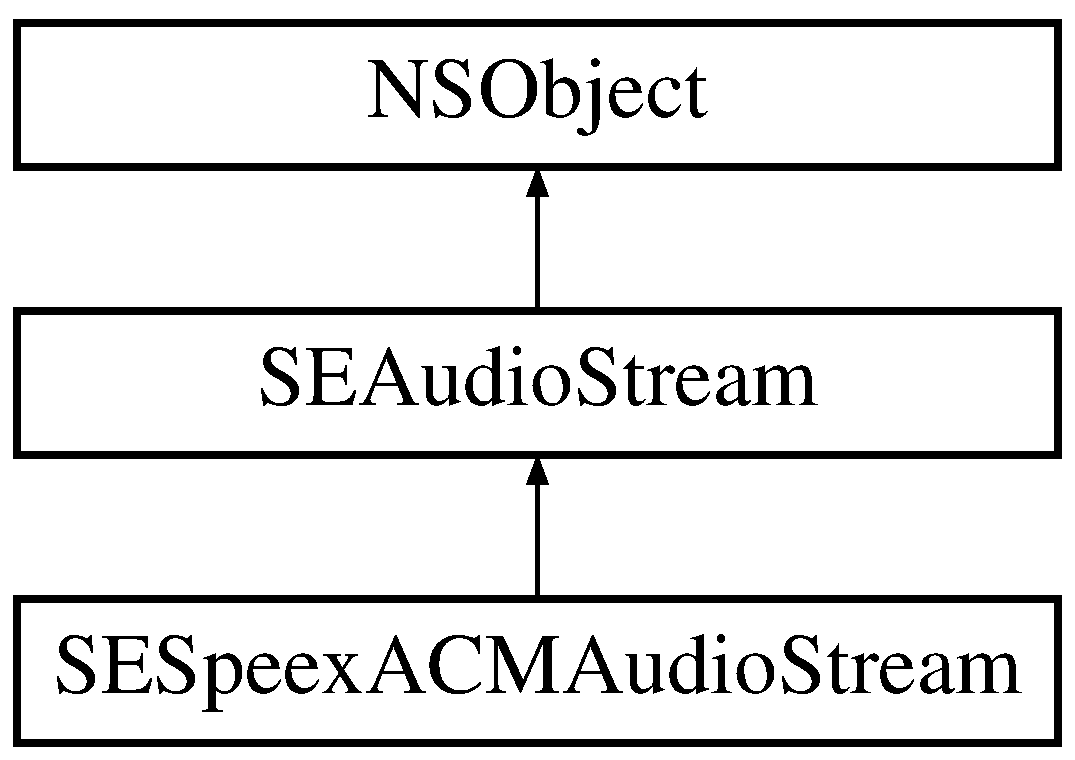
\includegraphics[height=3.000000cm]{interface_s_e_audio_stream}
\end{center}
\end{figure}
\subsection*{Instance Methods}
\begin{DoxyCompactItemize}
\item 
(id) -\/ \hyperlink{interface_s_e_audio_stream_adfb80527c355e64279d60a7b1af838ea}{init}
\item 
(id) -\/ \hyperlink{interface_s_e_audio_stream_a34663b1bbae1fdb5e32111a6629a994a}{init\-With\-Audio\-Stream\-:}
\item 
(id) -\/ \hyperlink{interface_s_e_audio_stream_a7acd0370d5f5066a6d00834af0eea200}{init\-With\-U\-R\-L\-:}
\item 
(id) -\/ \hyperlink{interface_s_e_audio_stream_a88b28dfe93892a08d261bd946beea26f}{init\-With\-Contents\-Of\-File\-:}
\item 
(void) -\/ \hyperlink{interface_s_e_audio_stream_add81dd9d9bd838f3a5dc1ceae94ccf26}{open}
\item 
(void) -\/ \hyperlink{interface_s_e_audio_stream_a8c4af367964e8be4817df12989f06d40}{close}
\item 
(void) -\/ \hyperlink{interface_s_e_audio_stream_ae59699f3f9cdf5fa000d9835da89e73e}{clear}
\item 
(void) -\/ \hyperlink{interface_s_e_audio_stream_a1dd26e76fbcd65f2d221f61de75fd3eb}{seek\-To\-Sample\-Position\-:}
\item 
(void) -\/ \hyperlink{interface_s_e_audio_stream_a720083efde7839f0a44ec7456805ffeb}{seek\-To\-Second\-:}
\item 
(void) -\/ \hyperlink{interface_s_e_audio_stream_ab721ccfe6c59695b85abc3fe00b37230}{exprort\-To\-File\-:completion\-:}
\item 
(N\-S\-Data $\ast$) -\/ \hyperlink{interface_s_e_audio_stream_a8d848d7a388d38fb670eb92e3bf6566d}{read\-Samples\-With\-Count\-:}
\item 
(N\-S\-Data $\ast$) -\/ \hyperlink{interface_s_e_audio_stream_a4501c22126f23cc1cb9ecbd1d7ddda6e}{read\-Samples\-From\-Channel\-:count\-:}
\item 
(void) -\/ \hyperlink{interface_s_e_audio_stream_ac80704c916ddbac8f8309f3a6a019e80}{read\-Samples\-:count\-:}
\item 
(void) -\/ \hyperlink{interface_s_e_audio_stream_ab184f74429643065a116a8f272bf79b3}{write\-Samples\-:}
\item 
(void) -\/ \hyperlink{interface_s_e_audio_stream_af19a129d2a78172d771f2552dd97f49b}{write\-Samples\-:count\-:}
\end{DoxyCompactItemize}
\subsection*{Properties}
\begin{DoxyCompactItemize}
\item 
Audio\-Stream\-Basic\-Description $\ast$ \hyperlink{interface_s_e_audio_stream_a96f11351b56bdd1d363ad05fb80d1a73}{audio\-Description}
\item 
N\-S\-Time\-Interval \hyperlink{interface_s_e_audio_stream_af5e4493693cf24fa25af34487993d693}{duration}
\item 
N\-S\-U\-R\-L $\ast$ \hyperlink{interface_s_e_audio_stream_a7561aaa75262c747a4da3d701e2094b9}{file\-Path\-U\-R\-L}
\item 
N\-S\-Error $\ast$ \hyperlink{interface_s_e_audio_stream_a095232a32323fc1b43568e1609cc934d}{error}
\item 
N\-S\-Integer \hyperlink{interface_s_e_audio_stream_a54229ab240455736790dad362c5335e1}{length}
\item 
N\-S\-Integer \hyperlink{interface_s_e_audio_stream_a1e8d0ba4849fffe376bcf5494987c9a8}{number\-Of\-Samples}
\item 
N\-S\-Integer \hyperlink{interface_s_e_audio_stream_afac964b9badc8642c250a2234eb3c044}{number\-Of\-Samples\-Per\-Channel}
\end{DoxyCompactItemize}


\subsection{Method Documentation}
\hypertarget{interface_s_e_audio_stream_ae59699f3f9cdf5fa000d9835da89e73e}{\index{S\-E\-Audio\-Stream@{S\-E\-Audio\-Stream}!clear@{clear}}
\index{clear@{clear}!SEAudioStream@{S\-E\-Audio\-Stream}}
\subsubsection[{clear}]{\setlength{\rightskip}{0pt plus 5cm}-\/ (void) clear 
\begin{DoxyParamCaption}
{}
\end{DoxyParamCaption}
}}\label{interface_s_e_audio_stream_ae59699f3f9cdf5fa000d9835da89e73e}
Delete all information in stream \hypertarget{interface_s_e_audio_stream_a8c4af367964e8be4817df12989f06d40}{\index{S\-E\-Audio\-Stream@{S\-E\-Audio\-Stream}!close@{close}}
\index{close@{close}!SEAudioStream@{S\-E\-Audio\-Stream}}
\subsubsection[{close}]{\setlength{\rightskip}{0pt plus 5cm}-\/ (void) close 
\begin{DoxyParamCaption}
{}
\end{DoxyParamCaption}
}}\label{interface_s_e_audio_stream_a8c4af367964e8be4817df12989f06d40}
Close Stream \hypertarget{interface_s_e_audio_stream_ab721ccfe6c59695b85abc3fe00b37230}{\index{S\-E\-Audio\-Stream@{S\-E\-Audio\-Stream}!exprort\-To\-File\-:completion\-:@{exprort\-To\-File\-:completion\-:}}
\index{exprort\-To\-File\-:completion\-:@{exprort\-To\-File\-:completion\-:}!SEAudioStream@{S\-E\-Audio\-Stream}}
\subsubsection[{exprort\-To\-File\-:completion\-:}]{\setlength{\rightskip}{0pt plus 5cm}-\/ (void) exprort\-To\-File\-: 
\begin{DoxyParamCaption}
\item[{(N\-S\-String$\ast$)}]{file\-Path}
\item[{completion:(void($^\wedge$)(N\-S\-Error$\ast$ {\bf error}))}]{completion}
\end{DoxyParamCaption}
}}\label{interface_s_e_audio_stream_ab721ccfe6c59695b85abc3fe00b37230}
Export all data to file \hypertarget{interface_s_e_audio_stream_adfb80527c355e64279d60a7b1af838ea}{\index{S\-E\-Audio\-Stream@{S\-E\-Audio\-Stream}!init@{init}}
\index{init@{init}!SEAudioStream@{S\-E\-Audio\-Stream}}
\subsubsection[{init}]{\setlength{\rightskip}{0pt plus 5cm}-\/ (id) init 
\begin{DoxyParamCaption}
{}
\end{DoxyParamCaption}
}}\label{interface_s_e_audio_stream_adfb80527c355e64279d60a7b1af838ea}
Create stream in memory \hypertarget{interface_s_e_audio_stream_a34663b1bbae1fdb5e32111a6629a994a}{\index{S\-E\-Audio\-Stream@{S\-E\-Audio\-Stream}!init\-With\-Audio\-Stream\-:@{init\-With\-Audio\-Stream\-:}}
\index{init\-With\-Audio\-Stream\-:@{init\-With\-Audio\-Stream\-:}!SEAudioStream@{S\-E\-Audio\-Stream}}
\subsubsection[{init\-With\-Audio\-Stream\-:}]{\setlength{\rightskip}{0pt plus 5cm}-\/ (id) init\-With\-Audio\-Stream\-: 
\begin{DoxyParamCaption}
\item[{({\bf S\-E\-Audio\-Stream}$\ast$)}]{stream}
\end{DoxyParamCaption}
}}\label{interface_s_e_audio_stream_a34663b1bbae1fdb5e32111a6629a994a}
Init with another audio stream \hypertarget{interface_s_e_audio_stream_a88b28dfe93892a08d261bd946beea26f}{\index{S\-E\-Audio\-Stream@{S\-E\-Audio\-Stream}!init\-With\-Contents\-Of\-File\-:@{init\-With\-Contents\-Of\-File\-:}}
\index{init\-With\-Contents\-Of\-File\-:@{init\-With\-Contents\-Of\-File\-:}!SEAudioStream@{S\-E\-Audio\-Stream}}
\subsubsection[{init\-With\-Contents\-Of\-File\-:}]{\setlength{\rightskip}{0pt plus 5cm}-\/ (id) init\-With\-Contents\-Of\-File\-: 
\begin{DoxyParamCaption}
\item[{(N\-S\-String$\ast$)}]{file}
\end{DoxyParamCaption}
}}\label{interface_s_e_audio_stream_a88b28dfe93892a08d261bd946beea26f}
Load from Storage \hypertarget{interface_s_e_audio_stream_a7acd0370d5f5066a6d00834af0eea200}{\index{S\-E\-Audio\-Stream@{S\-E\-Audio\-Stream}!init\-With\-U\-R\-L\-:@{init\-With\-U\-R\-L\-:}}
\index{init\-With\-U\-R\-L\-:@{init\-With\-U\-R\-L\-:}!SEAudioStream@{S\-E\-Audio\-Stream}}
\subsubsection[{init\-With\-U\-R\-L\-:}]{\setlength{\rightskip}{0pt plus 5cm}-\/ (id) init\-With\-U\-R\-L\-: 
\begin{DoxyParamCaption}
\item[{(N\-S\-String$\ast$)}]{url}
\end{DoxyParamCaption}
}}\label{interface_s_e_audio_stream_a7acd0370d5f5066a6d00834af0eea200}
Load from server \hypertarget{interface_s_e_audio_stream_add81dd9d9bd838f3a5dc1ceae94ccf26}{\index{S\-E\-Audio\-Stream@{S\-E\-Audio\-Stream}!open@{open}}
\index{open@{open}!SEAudioStream@{S\-E\-Audio\-Stream}}
\subsubsection[{open}]{\setlength{\rightskip}{0pt plus 5cm}-\/ (void) open 
\begin{DoxyParamCaption}
{}
\end{DoxyParamCaption}
}}\label{interface_s_e_audio_stream_add81dd9d9bd838f3a5dc1ceae94ccf26}
Open Stream \hypertarget{interface_s_e_audio_stream_ac80704c916ddbac8f8309f3a6a019e80}{\index{S\-E\-Audio\-Stream@{S\-E\-Audio\-Stream}!read\-Samples\-:count\-:@{read\-Samples\-:count\-:}}
\index{read\-Samples\-:count\-:@{read\-Samples\-:count\-:}!SEAudioStream@{S\-E\-Audio\-Stream}}
\subsubsection[{read\-Samples\-:count\-:}]{\setlength{\rightskip}{0pt plus 5cm}-\/ (void) read\-Samples\-: 
\begin{DoxyParamCaption}
\item[{(void $\ast$)}]{samples}
\item[{count:(N\-S\-Integer)}]{count}
\end{DoxyParamCaption}
}}\label{interface_s_e_audio_stream_ac80704c916ddbac8f8309f3a6a019e80}
Read Samples data 

Provided by category \hyperlink{category_s_e_audio_stream_07_read_08_ac80704c916ddbac8f8309f3a6a019e80}{S\-E\-Audio\-Stream(\-Read)}.

\hypertarget{interface_s_e_audio_stream_a4501c22126f23cc1cb9ecbd1d7ddda6e}{\index{S\-E\-Audio\-Stream@{S\-E\-Audio\-Stream}!read\-Samples\-From\-Channel\-:count\-:@{read\-Samples\-From\-Channel\-:count\-:}}
\index{read\-Samples\-From\-Channel\-:count\-:@{read\-Samples\-From\-Channel\-:count\-:}!SEAudioStream@{S\-E\-Audio\-Stream}}
\subsubsection[{read\-Samples\-From\-Channel\-:count\-:}]{\setlength{\rightskip}{0pt plus 5cm}-\/ (N\-S\-Data$\ast$) read\-Samples\-From\-Channel\-: 
\begin{DoxyParamCaption}
\item[{(N\-S\-Integer)}]{channels}
\item[{count:(N\-S\-Integer)}]{count}
\end{DoxyParamCaption}
}}\label{interface_s_e_audio_stream_a4501c22126f23cc1cb9ecbd1d7ddda6e}
Read Samples from one channel 

Provided by category \hyperlink{category_s_e_audio_stream_07_read_08_a4501c22126f23cc1cb9ecbd1d7ddda6e}{S\-E\-Audio\-Stream(\-Read)}.

\hypertarget{interface_s_e_audio_stream_a8d848d7a388d38fb670eb92e3bf6566d}{\index{S\-E\-Audio\-Stream@{S\-E\-Audio\-Stream}!read\-Samples\-With\-Count\-:@{read\-Samples\-With\-Count\-:}}
\index{read\-Samples\-With\-Count\-:@{read\-Samples\-With\-Count\-:}!SEAudioStream@{S\-E\-Audio\-Stream}}
\subsubsection[{read\-Samples\-With\-Count\-:}]{\setlength{\rightskip}{0pt plus 5cm}-\/ (N\-S\-Data$\ast$) read\-Samples\-With\-Count\-: 
\begin{DoxyParamCaption}
\item[{(N\-S\-Integer)}]{count}
\end{DoxyParamCaption}
}}\label{interface_s_e_audio_stream_a8d848d7a388d38fb670eb92e3bf6566d}
Read Samples from All Channels 

Provided by category \hyperlink{category_s_e_audio_stream_07_read_08_a8d848d7a388d38fb670eb92e3bf6566d}{S\-E\-Audio\-Stream(\-Read)}.

\hypertarget{interface_s_e_audio_stream_a1dd26e76fbcd65f2d221f61de75fd3eb}{\index{S\-E\-Audio\-Stream@{S\-E\-Audio\-Stream}!seek\-To\-Sample\-Position\-:@{seek\-To\-Sample\-Position\-:}}
\index{seek\-To\-Sample\-Position\-:@{seek\-To\-Sample\-Position\-:}!SEAudioStream@{S\-E\-Audio\-Stream}}
\subsubsection[{seek\-To\-Sample\-Position\-:}]{\setlength{\rightskip}{0pt plus 5cm}-\/ (void) seek\-To\-Sample\-Position\-: 
\begin{DoxyParamCaption}
\item[{(N\-S\-Integer)}]{position}
\end{DoxyParamCaption}
}}\label{interface_s_e_audio_stream_a1dd26e76fbcd65f2d221f61de75fd3eb}
Seek to position in samples include all channels \hypertarget{interface_s_e_audio_stream_a720083efde7839f0a44ec7456805ffeb}{\index{S\-E\-Audio\-Stream@{S\-E\-Audio\-Stream}!seek\-To\-Second\-:@{seek\-To\-Second\-:}}
\index{seek\-To\-Second\-:@{seek\-To\-Second\-:}!SEAudioStream@{S\-E\-Audio\-Stream}}
\subsubsection[{seek\-To\-Second\-:}]{\setlength{\rightskip}{0pt plus 5cm}-\/ (void) seek\-To\-Second\-: 
\begin{DoxyParamCaption}
\item[{(N\-S\-Time\-Interval)}]{second}
\end{DoxyParamCaption}
}}\label{interface_s_e_audio_stream_a720083efde7839f0a44ec7456805ffeb}
Seek to second \hypertarget{interface_s_e_audio_stream_ab184f74429643065a116a8f272bf79b3}{\index{S\-E\-Audio\-Stream@{S\-E\-Audio\-Stream}!write\-Samples\-:@{write\-Samples\-:}}
\index{write\-Samples\-:@{write\-Samples\-:}!SEAudioStream@{S\-E\-Audio\-Stream}}
\subsubsection[{write\-Samples\-:}]{\setlength{\rightskip}{0pt plus 5cm}-\/ (void) write\-Samples\-: 
\begin{DoxyParamCaption}
\item[{(N\-S\-Data $\ast$)}]{samples}
\end{DoxyParamCaption}
}}\label{interface_s_e_audio_stream_ab184f74429643065a116a8f272bf79b3}
Write Samples$\ast$ using N\-S\-Data 

Provided by category \hyperlink{category_s_e_audio_stream_07_write_08_ab184f74429643065a116a8f272bf79b3}{S\-E\-Audio\-Stream(\-Write)}.

\hypertarget{interface_s_e_audio_stream_af19a129d2a78172d771f2552dd97f49b}{\index{S\-E\-Audio\-Stream@{S\-E\-Audio\-Stream}!write\-Samples\-:count\-:@{write\-Samples\-:count\-:}}
\index{write\-Samples\-:count\-:@{write\-Samples\-:count\-:}!SEAudioStream@{S\-E\-Audio\-Stream}}
\subsubsection[{write\-Samples\-:count\-:}]{\setlength{\rightskip}{0pt plus 5cm}-\/ (void) {\bf write\-Samples\-:} 
\begin{DoxyParamCaption}
\item[{(void $\ast$)}]{data}
\item[{count:(N\-S\-Integer)}]{count}
\end{DoxyParamCaption}
}}\label{interface_s_e_audio_stream_af19a129d2a78172d771f2552dd97f49b}
Write Samples using data 

Provided by category \hyperlink{category_s_e_audio_stream_07_write_08_af19a129d2a78172d771f2552dd97f49b}{S\-E\-Audio\-Stream(\-Write)}.



\subsection{Property Documentation}
\hypertarget{interface_s_e_audio_stream_a96f11351b56bdd1d363ad05fb80d1a73}{\index{S\-E\-Audio\-Stream@{S\-E\-Audio\-Stream}!audio\-Description@{audio\-Description}}
\index{audio\-Description@{audio\-Description}!SEAudioStream@{S\-E\-Audio\-Stream}}
\subsubsection[{audio\-Description}]{\setlength{\rightskip}{0pt plus 5cm}-\/ (Audio\-Stream\-Basic\-Description$\ast$) audio\-Description\hspace{0.3cm}{\ttfamily [read]}, {\ttfamily [write]}, {\ttfamily [nonatomic]}, {\ttfamily [assign]}}}\label{interface_s_e_audio_stream_a96f11351b56bdd1d363ad05fb80d1a73}
Audio File Description \hypertarget{interface_s_e_audio_stream_af5e4493693cf24fa25af34487993d693}{\index{S\-E\-Audio\-Stream@{S\-E\-Audio\-Stream}!duration@{duration}}
\index{duration@{duration}!SEAudioStream@{S\-E\-Audio\-Stream}}
\subsubsection[{duration}]{\setlength{\rightskip}{0pt plus 5cm}-\/ (N\-S\-Time\-Interval) duration\hspace{0.3cm}{\ttfamily [read]}, {\ttfamily [nonatomic]}, {\ttfamily [assign]}}}\label{interface_s_e_audio_stream_af5e4493693cf24fa25af34487993d693}
Audio Duration$\ast$ \hypertarget{interface_s_e_audio_stream_a095232a32323fc1b43568e1609cc934d}{\index{S\-E\-Audio\-Stream@{S\-E\-Audio\-Stream}!error@{error}}
\index{error@{error}!SEAudioStream@{S\-E\-Audio\-Stream}}
\subsubsection[{error}]{\setlength{\rightskip}{0pt plus 5cm}-\/ (N\-S\-Error$\ast$) error\hspace{0.3cm}{\ttfamily [read]}, {\ttfamily [nonatomic]}, {\ttfamily [assign]}}}\label{interface_s_e_audio_stream_a095232a32323fc1b43568e1609cc934d}
Last Error \hypertarget{interface_s_e_audio_stream_a7561aaa75262c747a4da3d701e2094b9}{\index{S\-E\-Audio\-Stream@{S\-E\-Audio\-Stream}!file\-Path\-U\-R\-L@{file\-Path\-U\-R\-L}}
\index{file\-Path\-U\-R\-L@{file\-Path\-U\-R\-L}!SEAudioStream@{S\-E\-Audio\-Stream}}
\subsubsection[{file\-Path\-U\-R\-L}]{\setlength{\rightskip}{0pt plus 5cm}-\/ (N\-S\-U\-R\-L$\ast$) file\-Path\-U\-R\-L\hspace{0.3cm}{\ttfamily [read]}, {\ttfamily [nonatomic]}, {\ttfamily [assign]}}}\label{interface_s_e_audio_stream_a7561aaa75262c747a4da3d701e2094b9}
File Path \hypertarget{interface_s_e_audio_stream_a54229ab240455736790dad362c5335e1}{\index{S\-E\-Audio\-Stream@{S\-E\-Audio\-Stream}!length@{length}}
\index{length@{length}!SEAudioStream@{S\-E\-Audio\-Stream}}
\subsubsection[{length}]{\setlength{\rightskip}{0pt plus 5cm}-\/ (N\-S\-Integer) length\hspace{0.3cm}{\ttfamily [read]}, {\ttfamily [nonatomic]}, {\ttfamily [assign]}}}\label{interface_s_e_audio_stream_a54229ab240455736790dad362c5335e1}
Stream Length in bytes \hypertarget{interface_s_e_audio_stream_a1e8d0ba4849fffe376bcf5494987c9a8}{\index{S\-E\-Audio\-Stream@{S\-E\-Audio\-Stream}!number\-Of\-Samples@{number\-Of\-Samples}}
\index{number\-Of\-Samples@{number\-Of\-Samples}!SEAudioStream@{S\-E\-Audio\-Stream}}
\subsubsection[{number\-Of\-Samples}]{\setlength{\rightskip}{0pt plus 5cm}-\/ (N\-S\-Integer) number\-Of\-Samples\hspace{0.3cm}{\ttfamily [read]}, {\ttfamily [nonatomic]}, {\ttfamily [assign]}}}\label{interface_s_e_audio_stream_a1e8d0ba4849fffe376bcf5494987c9a8}
Number of samples including all channels \hypertarget{interface_s_e_audio_stream_afac964b9badc8642c250a2234eb3c044}{\index{S\-E\-Audio\-Stream@{S\-E\-Audio\-Stream}!number\-Of\-Samples\-Per\-Channel@{number\-Of\-Samples\-Per\-Channel}}
\index{number\-Of\-Samples\-Per\-Channel@{number\-Of\-Samples\-Per\-Channel}!SEAudioStream@{S\-E\-Audio\-Stream}}
\subsubsection[{number\-Of\-Samples\-Per\-Channel}]{\setlength{\rightskip}{0pt plus 5cm}-\/ (N\-S\-Integer) number\-Of\-Samples\-Per\-Channel\hspace{0.3cm}{\ttfamily [read]}, {\ttfamily [nonatomic]}, {\ttfamily [assign]}}}\label{interface_s_e_audio_stream_afac964b9badc8642c250a2234eb3c044}
Number of samples per channel 

The documentation for this class was generated from the following files\-:\begin{DoxyCompactItemize}
\item 
/\-Users/igor/\-Develop/\-Develop\-Git/\-Davacon/i\-Phone/\-Sound\-Recorder/\-Classes/\-Core/\-Sound\-Editor/\hyperlink{_s_e_audio_stream_8h}{S\-E\-Audio\-Stream.\-h}\item 
/\-Users/igor/\-Develop/\-Develop\-Git/\-Davacon/i\-Phone/\-Sound\-Recorder/\-Classes/\-Core/\-Sound\-Editor/\hyperlink{_s_e_audio_stream_8m}{S\-E\-Audio\-Stream.\-m}\end{DoxyCompactItemize}

\hypertarget{category_s_e_audio_stream_07_08}{\section{S\-E\-Audio\-Stream() Category Reference}
\label{category_s_e_audio_stream_07_08}\index{S\-E\-Audio\-Stream()@{S\-E\-Audio\-Stream()}}
}
\subsection*{Instance Methods}
\begin{DoxyCompactItemize}
\item 
(void) -\/ \hyperlink{category_s_e_audio_stream_07_08_ad24e56ffa5a11921036f512b30c2e61d}{pm\-\_\-perform\-Error\-:}
\item 
(void) -\/ \hyperlink{category_s_e_audio_stream_07_08_a9e38c18656273234be61619aafa089e6}{pm\-\_\-handle\-Property\-Change\-For\-File\-Stream\-:file\-Stream\-Property\-I\-D\-:io\-Flags\-:}
\item 
(void) -\/ \hyperlink{category_s_e_audio_stream_07_08_a0e5ee17bc631e7b9b6cc2d710d855d1d}{pm\-\_\-handle\-Audio\-Packets\-:number\-Bytes\-:number\-Packets\-:packet\-Descriptions\-:}
\item 
(B\-O\-O\-L) -\/ \hyperlink{category_s_e_audio_stream_07_08_aa7990eeb00de4c75445968be37c3fb6c}{pm\-\_\-read\-Header}
\item 
(N\-S\-Time\-Interval) -\/ \hyperlink{category_s_e_audio_stream_07_08_a6d445c53ea91dc93dc816d869a0920ca}{pm\-\_\-data\-Duration}
\item 
(B\-O\-O\-L) -\/ \hyperlink{category_s_e_audio_stream_07_08_a70ebad17a61f0c4638e165b1ab698f12}{pm\-\_\-flush}
\end{DoxyCompactItemize}
\subsection*{Class Methods}
\begin{DoxyCompactItemize}
\item 
(Audio\-File\-Type\-I\-D) + \hyperlink{category_s_e_audio_stream_07_08_a12c6083989cd11b11dbd2358af3db5b1}{pm\-\_\-hint\-For\-File\-Extension\-:}
\end{DoxyCompactItemize}
\subsection*{Properties}
\begin{DoxyCompactItemize}
\item 
\hyperlink{_s_e_audio_stream_8h_a9689aa516925fa132495c3c8a719ba57}{T\-S\-E\-Audio\-Stream\-Mode} \hyperlink{category_s_e_audio_stream_07_08_ab3ea1257ebd508183804d76b4fabb59a}{pv\-\_\-mode}
\item 
\hyperlink{_s_e_audio_stream_8m_ab23d772523cd805a49196d237af16aa2}{T\-S\-E\-Audio\-Stream\-Source\-Type} \hyperlink{category_s_e_audio_stream_07_08_ab41d2bb3f3368b5d2e59f26bfb63f108}{pv\-\_\-type}
\item 
N\-S\-Mutable\-Data $\ast$ \hyperlink{category_s_e_audio_stream_07_08_a47ec9fee0bc8fe3ed1fedbb5bf3659de}{pv\-\_\-data}
\item 
\hyperlink{interface_s_e_audio_stream}{S\-E\-Audio\-Stream} $\ast$ \hyperlink{category_s_e_audio_stream_07_08_aa149aa8c3150db2e972f656382b276be}{pv\-\_\-other\-Audio\-Stream}
\item 
N\-S\-U\-R\-L $\ast$ \hyperlink{category_s_e_audio_stream_07_08_ac5062bf935bfe512908c148b64ebaa84}{pv\-\_\-url}
\item 
N\-S\-Error $\ast$ \hyperlink{category_s_e_audio_stream_07_08_a43937aa5b15468780d7b4e582c690366}{pv\-\_\-error}
\item 
Audio\-File\-Stream\-I\-D \hyperlink{category_s_e_audio_stream_07_08_a3d66ea999bebad5a9048f2f019ad7e9a}{pv\-\_\-audio\-File\-Stream}
\item 
N\-S\-File\-Handle $\ast$ \hyperlink{category_s_e_audio_stream_07_08_a4b5eb36068a2815dae1d2236824aea74}{pv\-\_\-file\-Handle}
\item 
Audio\-Stream\-Basic\-Description \hyperlink{category_s_e_audio_stream_07_08_a27b75ce98f8fe681b6de1b27ecc39df9}{pv\-\_\-audio\-Description}
\item 
N\-S\-U\-Integer \hyperlink{category_s_e_audio_stream_07_08_a908e9b0330fba1110c9ef04d26494729}{pv\-\_\-data\-Length}
\item 
N\-S\-U\-Integer \hyperlink{category_s_e_audio_stream_07_08_ac36ec8eab9c05e43ab0907663c3d172f}{pv\-\_\-data\-Offset}
\item 
Audio\-File\-Type\-I\-D \hyperlink{category_s_e_audio_stream_07_08_a7f4dc2a06927994d828cf7d7b52918be}{pv\-\_\-hint}
\item 
Audio\-File\-I\-D \hyperlink{category_s_e_audio_stream_07_08_a63651ad03f9f237a9bce2449ad37de67}{pv\-\_\-write\-File}
\end{DoxyCompactItemize}


\subsection{Method Documentation}
\hypertarget{category_s_e_audio_stream_07_08_a6d445c53ea91dc93dc816d869a0920ca}{\index{S\-E\-Audio\-Stream()@{S\-E\-Audio\-Stream()}!pm\-\_\-data\-Duration@{pm\-\_\-data\-Duration}}
\index{pm\-\_\-data\-Duration@{pm\-\_\-data\-Duration}!SEAudioStream()@{S\-E\-Audio\-Stream()}}
\subsubsection[{pm\-\_\-data\-Duration}]{\setlength{\rightskip}{0pt plus 5cm}-\/ (N\-S\-Time\-Interval) pm\-\_\-data\-Duration 
\begin{DoxyParamCaption}
{}
\end{DoxyParamCaption}
}}\label{category_s_e_audio_stream_07_08_a6d445c53ea91dc93dc816d869a0920ca}
\hypertarget{category_s_e_audio_stream_07_08_a70ebad17a61f0c4638e165b1ab698f12}{\index{S\-E\-Audio\-Stream()@{S\-E\-Audio\-Stream()}!pm\-\_\-flush@{pm\-\_\-flush}}
\index{pm\-\_\-flush@{pm\-\_\-flush}!SEAudioStream()@{S\-E\-Audio\-Stream()}}
\subsubsection[{pm\-\_\-flush}]{\setlength{\rightskip}{0pt plus 5cm}-\/ (B\-O\-O\-L) pm\-\_\-flush 
\begin{DoxyParamCaption}
{}
\end{DoxyParamCaption}
}}\label{category_s_e_audio_stream_07_08_a70ebad17a61f0c4638e165b1ab698f12}
\hypertarget{category_s_e_audio_stream_07_08_a0e5ee17bc631e7b9b6cc2d710d855d1d}{\index{S\-E\-Audio\-Stream()@{S\-E\-Audio\-Stream()}!pm\-\_\-handle\-Audio\-Packets\-:number\-Bytes\-:number\-Packets\-:packet\-Descriptions\-:@{pm\-\_\-handle\-Audio\-Packets\-:number\-Bytes\-:number\-Packets\-:packet\-Descriptions\-:}}
\index{pm\-\_\-handle\-Audio\-Packets\-:number\-Bytes\-:number\-Packets\-:packet\-Descriptions\-:@{pm\-\_\-handle\-Audio\-Packets\-:number\-Bytes\-:number\-Packets\-:packet\-Descriptions\-:}!SEAudioStream()@{S\-E\-Audio\-Stream()}}
\subsubsection[{pm\-\_\-handle\-Audio\-Packets\-:number\-Bytes\-:number\-Packets\-:packet\-Descriptions\-:}]{\setlength{\rightskip}{0pt plus 5cm}-\/ (void) pm\-\_\-handle\-Audio\-Packets\-: 
\begin{DoxyParamCaption}
\item[{(const void $\ast$)}]{in\-Input\-Data}
\item[{numberBytes:(U\-Int32)}]{in\-Number\-Bytes}
\item[{numberPackets:(U\-Int32)}]{in\-Number\-Packets}
\item[{packetDescriptions:(Audio\-Stream\-Packet\-Description $\ast$)}]{in\-Packet\-Descriptions}
\end{DoxyParamCaption}
}}\label{category_s_e_audio_stream_07_08_a0e5ee17bc631e7b9b6cc2d710d855d1d}
\hypertarget{category_s_e_audio_stream_07_08_a9e38c18656273234be61619aafa089e6}{\index{S\-E\-Audio\-Stream()@{S\-E\-Audio\-Stream()}!pm\-\_\-handle\-Property\-Change\-For\-File\-Stream\-:file\-Stream\-Property\-I\-D\-:io\-Flags\-:@{pm\-\_\-handle\-Property\-Change\-For\-File\-Stream\-:file\-Stream\-Property\-I\-D\-:io\-Flags\-:}}
\index{pm\-\_\-handle\-Property\-Change\-For\-File\-Stream\-:file\-Stream\-Property\-I\-D\-:io\-Flags\-:@{pm\-\_\-handle\-Property\-Change\-For\-File\-Stream\-:file\-Stream\-Property\-I\-D\-:io\-Flags\-:}!SEAudioStream()@{S\-E\-Audio\-Stream()}}
\subsubsection[{pm\-\_\-handle\-Property\-Change\-For\-File\-Stream\-:file\-Stream\-Property\-I\-D\-:io\-Flags\-:}]{\setlength{\rightskip}{0pt plus 5cm}-\/ (void) pm\-\_\-handle\-Property\-Change\-For\-File\-Stream\-: 
\begin{DoxyParamCaption}
\item[{(Audio\-File\-Stream\-I\-D)}]{in\-Audio\-File\-Stream}
\item[{fileStreamPropertyID:(Audio\-File\-Stream\-Property\-I\-D)}]{in\-Property\-I\-D}
\item[{ioFlags:(U\-Int32 $\ast$)}]{io\-Flags}
\end{DoxyParamCaption}
}}\label{category_s_e_audio_stream_07_08_a9e38c18656273234be61619aafa089e6}
\hypertarget{category_s_e_audio_stream_07_08_a12c6083989cd11b11dbd2358af3db5b1}{\index{S\-E\-Audio\-Stream()@{S\-E\-Audio\-Stream()}!pm\-\_\-hint\-For\-File\-Extension\-:@{pm\-\_\-hint\-For\-File\-Extension\-:}}
\index{pm\-\_\-hint\-For\-File\-Extension\-:@{pm\-\_\-hint\-For\-File\-Extension\-:}!SEAudioStream()@{S\-E\-Audio\-Stream()}}
\subsubsection[{pm\-\_\-hint\-For\-File\-Extension\-:}]{\setlength{\rightskip}{0pt plus 5cm}+ (Audio\-File\-Type\-I\-D) pm\-\_\-hint\-For\-File\-Extension\-: 
\begin{DoxyParamCaption}
\item[{(N\-S\-String $\ast$)}]{file\-Extension}
\end{DoxyParamCaption}
}}\label{category_s_e_audio_stream_07_08_a12c6083989cd11b11dbd2358af3db5b1}
\hypertarget{category_s_e_audio_stream_07_08_ad24e56ffa5a11921036f512b30c2e61d}{\index{S\-E\-Audio\-Stream()@{S\-E\-Audio\-Stream()}!pm\-\_\-perform\-Error\-:@{pm\-\_\-perform\-Error\-:}}
\index{pm\-\_\-perform\-Error\-:@{pm\-\_\-perform\-Error\-:}!SEAudioStream()@{S\-E\-Audio\-Stream()}}
\subsubsection[{pm\-\_\-perform\-Error\-:}]{\setlength{\rightskip}{0pt plus 5cm}-\/ (void) pm\-\_\-perform\-Error\-: 
\begin{DoxyParamCaption}
\item[{({\bf T\-S\-E\-Audio\-Stream\-Status\-Type})}]{status\-Type}
\end{DoxyParamCaption}
}}\label{category_s_e_audio_stream_07_08_ad24e56ffa5a11921036f512b30c2e61d}
\hypertarget{category_s_e_audio_stream_07_08_aa7990eeb00de4c75445968be37c3fb6c}{\index{S\-E\-Audio\-Stream()@{S\-E\-Audio\-Stream()}!pm\-\_\-read\-Header@{pm\-\_\-read\-Header}}
\index{pm\-\_\-read\-Header@{pm\-\_\-read\-Header}!SEAudioStream()@{S\-E\-Audio\-Stream()}}
\subsubsection[{pm\-\_\-read\-Header}]{\setlength{\rightskip}{0pt plus 5cm}-\/ (B\-O\-O\-L) pm\-\_\-read\-Header 
\begin{DoxyParamCaption}
{}
\end{DoxyParamCaption}
}}\label{category_s_e_audio_stream_07_08_aa7990eeb00de4c75445968be37c3fb6c}


\subsection{Property Documentation}
\hypertarget{category_s_e_audio_stream_07_08_a27b75ce98f8fe681b6de1b27ecc39df9}{\index{S\-E\-Audio\-Stream()@{S\-E\-Audio\-Stream()}!pv\-\_\-audio\-Description@{pv\-\_\-audio\-Description}}
\index{pv\-\_\-audio\-Description@{pv\-\_\-audio\-Description}!SEAudioStream()@{S\-E\-Audio\-Stream()}}
\subsubsection[{pv\-\_\-audio\-Description}]{\setlength{\rightskip}{0pt plus 5cm}-\/ (Audio\-Stream\-Basic\-Description) pv\-\_\-audio\-Description\hspace{0.3cm}{\ttfamily [read]}, {\ttfamily [write]}, {\ttfamily [nonatomic]}, {\ttfamily [assign]}}}\label{category_s_e_audio_stream_07_08_a27b75ce98f8fe681b6de1b27ecc39df9}
\hypertarget{category_s_e_audio_stream_07_08_a3d66ea999bebad5a9048f2f019ad7e9a}{\index{S\-E\-Audio\-Stream()@{S\-E\-Audio\-Stream()}!pv\-\_\-audio\-File\-Stream@{pv\-\_\-audio\-File\-Stream}}
\index{pv\-\_\-audio\-File\-Stream@{pv\-\_\-audio\-File\-Stream}!SEAudioStream()@{S\-E\-Audio\-Stream()}}
\subsubsection[{pv\-\_\-audio\-File\-Stream}]{\setlength{\rightskip}{0pt plus 5cm}-\/ (Audio\-File\-Stream\-I\-D) pv\-\_\-audio\-File\-Stream\hspace{0.3cm}{\ttfamily [read]}, {\ttfamily [write]}, {\ttfamily [nonatomic]}, {\ttfamily [assign]}}}\label{category_s_e_audio_stream_07_08_a3d66ea999bebad5a9048f2f019ad7e9a}
\hypertarget{category_s_e_audio_stream_07_08_a47ec9fee0bc8fe3ed1fedbb5bf3659de}{\index{S\-E\-Audio\-Stream()@{S\-E\-Audio\-Stream()}!pv\-\_\-data@{pv\-\_\-data}}
\index{pv\-\_\-data@{pv\-\_\-data}!SEAudioStream()@{S\-E\-Audio\-Stream()}}
\subsubsection[{pv\-\_\-data}]{\setlength{\rightskip}{0pt plus 5cm}-\/ (N\-S\-Mutable\-Data$\ast$) pv\-\_\-data\hspace{0.3cm}{\ttfamily [read]}, {\ttfamily [write]}, {\ttfamily [nonatomic]}, {\ttfamily [strong]}}}\label{category_s_e_audio_stream_07_08_a47ec9fee0bc8fe3ed1fedbb5bf3659de}
\hypertarget{category_s_e_audio_stream_07_08_a908e9b0330fba1110c9ef04d26494729}{\index{S\-E\-Audio\-Stream()@{S\-E\-Audio\-Stream()}!pv\-\_\-data\-Length@{pv\-\_\-data\-Length}}
\index{pv\-\_\-data\-Length@{pv\-\_\-data\-Length}!SEAudioStream()@{S\-E\-Audio\-Stream()}}
\subsubsection[{pv\-\_\-data\-Length}]{\setlength{\rightskip}{0pt plus 5cm}-\/ (N\-S\-U\-Integer) pv\-\_\-data\-Length\hspace{0.3cm}{\ttfamily [read]}, {\ttfamily [write]}, {\ttfamily [nonatomic]}, {\ttfamily [assign]}}}\label{category_s_e_audio_stream_07_08_a908e9b0330fba1110c9ef04d26494729}
\hypertarget{category_s_e_audio_stream_07_08_ac36ec8eab9c05e43ab0907663c3d172f}{\index{S\-E\-Audio\-Stream()@{S\-E\-Audio\-Stream()}!pv\-\_\-data\-Offset@{pv\-\_\-data\-Offset}}
\index{pv\-\_\-data\-Offset@{pv\-\_\-data\-Offset}!SEAudioStream()@{S\-E\-Audio\-Stream()}}
\subsubsection[{pv\-\_\-data\-Offset}]{\setlength{\rightskip}{0pt plus 5cm}-\/ (N\-S\-U\-Integer) pv\-\_\-data\-Offset\hspace{0.3cm}{\ttfamily [read]}, {\ttfamily [write]}, {\ttfamily [nonatomic]}, {\ttfamily [assign]}}}\label{category_s_e_audio_stream_07_08_ac36ec8eab9c05e43ab0907663c3d172f}
\hypertarget{category_s_e_audio_stream_07_08_a43937aa5b15468780d7b4e582c690366}{\index{S\-E\-Audio\-Stream()@{S\-E\-Audio\-Stream()}!pv\-\_\-error@{pv\-\_\-error}}
\index{pv\-\_\-error@{pv\-\_\-error}!SEAudioStream()@{S\-E\-Audio\-Stream()}}
\subsubsection[{pv\-\_\-error}]{\setlength{\rightskip}{0pt plus 5cm}-\/ (N\-S\-Error$\ast$) pv\-\_\-error\hspace{0.3cm}{\ttfamily [read]}, {\ttfamily [write]}, {\ttfamily [nonatomic]}, {\ttfamily [strong]}}}\label{category_s_e_audio_stream_07_08_a43937aa5b15468780d7b4e582c690366}
\hypertarget{category_s_e_audio_stream_07_08_a4b5eb36068a2815dae1d2236824aea74}{\index{S\-E\-Audio\-Stream()@{S\-E\-Audio\-Stream()}!pv\-\_\-file\-Handle@{pv\-\_\-file\-Handle}}
\index{pv\-\_\-file\-Handle@{pv\-\_\-file\-Handle}!SEAudioStream()@{S\-E\-Audio\-Stream()}}
\subsubsection[{pv\-\_\-file\-Handle}]{\setlength{\rightskip}{0pt plus 5cm}-\/ (N\-S\-File\-Handle$\ast$) pv\-\_\-file\-Handle\hspace{0.3cm}{\ttfamily [read]}, {\ttfamily [write]}, {\ttfamily [nonatomic]}, {\ttfamily [strong]}}}\label{category_s_e_audio_stream_07_08_a4b5eb36068a2815dae1d2236824aea74}
\hypertarget{category_s_e_audio_stream_07_08_a7f4dc2a06927994d828cf7d7b52918be}{\index{S\-E\-Audio\-Stream()@{S\-E\-Audio\-Stream()}!pv\-\_\-hint@{pv\-\_\-hint}}
\index{pv\-\_\-hint@{pv\-\_\-hint}!SEAudioStream()@{S\-E\-Audio\-Stream()}}
\subsubsection[{pv\-\_\-hint}]{\setlength{\rightskip}{0pt plus 5cm}-\/ (Audio\-File\-Type\-I\-D) pv\-\_\-hint\hspace{0.3cm}{\ttfamily [read]}, {\ttfamily [write]}, {\ttfamily [nonatomic]}, {\ttfamily [assign]}}}\label{category_s_e_audio_stream_07_08_a7f4dc2a06927994d828cf7d7b52918be}
\hypertarget{category_s_e_audio_stream_07_08_ab3ea1257ebd508183804d76b4fabb59a}{\index{S\-E\-Audio\-Stream()@{S\-E\-Audio\-Stream()}!pv\-\_\-mode@{pv\-\_\-mode}}
\index{pv\-\_\-mode@{pv\-\_\-mode}!SEAudioStream()@{S\-E\-Audio\-Stream()}}
\subsubsection[{pv\-\_\-mode}]{\setlength{\rightskip}{0pt plus 5cm}-\/ ({\bf T\-S\-E\-Audio\-Stream\-Mode}) pv\-\_\-mode\hspace{0.3cm}{\ttfamily [read]}, {\ttfamily [write]}, {\ttfamily [nonatomic]}, {\ttfamily [assign]}}}\label{category_s_e_audio_stream_07_08_ab3ea1257ebd508183804d76b4fabb59a}
\hypertarget{category_s_e_audio_stream_07_08_aa149aa8c3150db2e972f656382b276be}{\index{S\-E\-Audio\-Stream()@{S\-E\-Audio\-Stream()}!pv\-\_\-other\-Audio\-Stream@{pv\-\_\-other\-Audio\-Stream}}
\index{pv\-\_\-other\-Audio\-Stream@{pv\-\_\-other\-Audio\-Stream}!SEAudioStream()@{S\-E\-Audio\-Stream()}}
\subsubsection[{pv\-\_\-other\-Audio\-Stream}]{\setlength{\rightskip}{0pt plus 5cm}-\/ ({\bf S\-E\-Audio\-Stream}$\ast$) pv\-\_\-other\-Audio\-Stream\hspace{0.3cm}{\ttfamily [read]}, {\ttfamily [write]}, {\ttfamily [nonatomic]}, {\ttfamily [strong]}}}\label{category_s_e_audio_stream_07_08_aa149aa8c3150db2e972f656382b276be}
\hypertarget{category_s_e_audio_stream_07_08_ab41d2bb3f3368b5d2e59f26bfb63f108}{\index{S\-E\-Audio\-Stream()@{S\-E\-Audio\-Stream()}!pv\-\_\-type@{pv\-\_\-type}}
\index{pv\-\_\-type@{pv\-\_\-type}!SEAudioStream()@{S\-E\-Audio\-Stream()}}
\subsubsection[{pv\-\_\-type}]{\setlength{\rightskip}{0pt plus 5cm}-\/ ({\bf T\-S\-E\-Audio\-Stream\-Source\-Type}) pv\-\_\-type\hspace{0.3cm}{\ttfamily [read]}, {\ttfamily [write]}, {\ttfamily [nonatomic]}, {\ttfamily [assign]}}}\label{category_s_e_audio_stream_07_08_ab41d2bb3f3368b5d2e59f26bfb63f108}
\hypertarget{category_s_e_audio_stream_07_08_ac5062bf935bfe512908c148b64ebaa84}{\index{S\-E\-Audio\-Stream()@{S\-E\-Audio\-Stream()}!pv\-\_\-url@{pv\-\_\-url}}
\index{pv\-\_\-url@{pv\-\_\-url}!SEAudioStream()@{S\-E\-Audio\-Stream()}}
\subsubsection[{pv\-\_\-url}]{\setlength{\rightskip}{0pt plus 5cm}-\/ (N\-S\-U\-R\-L$\ast$) pv\-\_\-url\hspace{0.3cm}{\ttfamily [read]}, {\ttfamily [write]}, {\ttfamily [nonatomic]}, {\ttfamily [strong]}}}\label{category_s_e_audio_stream_07_08_ac5062bf935bfe512908c148b64ebaa84}
\hypertarget{category_s_e_audio_stream_07_08_a63651ad03f9f237a9bce2449ad37de67}{\index{S\-E\-Audio\-Stream()@{S\-E\-Audio\-Stream()}!pv\-\_\-write\-File@{pv\-\_\-write\-File}}
\index{pv\-\_\-write\-File@{pv\-\_\-write\-File}!SEAudioStream()@{S\-E\-Audio\-Stream()}}
\subsubsection[{pv\-\_\-write\-File}]{\setlength{\rightskip}{0pt plus 5cm}-\/ (Audio\-File\-I\-D) pv\-\_\-write\-File\hspace{0.3cm}{\ttfamily [read]}, {\ttfamily [write]}, {\ttfamily [nonatomic]}, {\ttfamily [assign]}}}\label{category_s_e_audio_stream_07_08_a63651ad03f9f237a9bce2449ad37de67}


The documentation for this category was generated from the following file\-:\begin{DoxyCompactItemize}
\item 
/\-Users/igor/\-Develop/\-Develop\-Git/\-Davacon/i\-Phone/\-Sound\-Recorder/\-Classes/\-Core/\-Sound\-Editor/\hyperlink{_s_e_audio_stream_8m}{S\-E\-Audio\-Stream.\-m}\end{DoxyCompactItemize}

\hypertarget{category_s_e_audio_stream_07_read_08}{\section{S\-E\-Audio\-Stream(Read) Category Reference}
\label{category_s_e_audio_stream_07_read_08}\index{S\-E\-Audio\-Stream(\-Read)@{S\-E\-Audio\-Stream(\-Read)}}
}


{\ttfamily \#import $<$S\-E\-Audio\-Stream.\-h$>$}

\subsection*{Instance Methods}
\begin{DoxyCompactItemize}
\item 
(N\-S\-Data $\ast$) -\/ \hyperlink{category_s_e_audio_stream_07_read_08_a8d848d7a388d38fb670eb92e3bf6566d}{read\-Samples\-With\-Count\-:}
\item 
(N\-S\-Data $\ast$) -\/ \hyperlink{category_s_e_audio_stream_07_read_08_a4501c22126f23cc1cb9ecbd1d7ddda6e}{read\-Samples\-From\-Channel\-:count\-:}
\item 
(void) -\/ \hyperlink{category_s_e_audio_stream_07_read_08_ac80704c916ddbac8f8309f3a6a019e80}{read\-Samples\-:count\-:}
\end{DoxyCompactItemize}


\subsection{Method Documentation}
\hypertarget{category_s_e_audio_stream_07_read_08_ac80704c916ddbac8f8309f3a6a019e80}{\index{S\-E\-Audio\-Stream(\-Read)@{S\-E\-Audio\-Stream(\-Read)}!read\-Samples\-:count\-:@{read\-Samples\-:count\-:}}
\index{read\-Samples\-:count\-:@{read\-Samples\-:count\-:}!SEAudioStream(Read)@{S\-E\-Audio\-Stream(\-Read)}}
\subsubsection[{read\-Samples\-:count\-:}]{\setlength{\rightskip}{0pt plus 5cm}-\/ (void) read\-Samples\-: 
\begin{DoxyParamCaption}
\item[{(void $\ast$)}]{samples}
\item[{count:(N\-S\-Integer)}]{count}
\end{DoxyParamCaption}
}}\label{category_s_e_audio_stream_07_read_08_ac80704c916ddbac8f8309f3a6a019e80}
Read Samples data 

Extends class \hyperlink{interface_s_e_audio_stream_ac80704c916ddbac8f8309f3a6a019e80}{S\-E\-Audio\-Stream}.

\hypertarget{category_s_e_audio_stream_07_read_08_a4501c22126f23cc1cb9ecbd1d7ddda6e}{\index{S\-E\-Audio\-Stream(\-Read)@{S\-E\-Audio\-Stream(\-Read)}!read\-Samples\-From\-Channel\-:count\-:@{read\-Samples\-From\-Channel\-:count\-:}}
\index{read\-Samples\-From\-Channel\-:count\-:@{read\-Samples\-From\-Channel\-:count\-:}!SEAudioStream(Read)@{S\-E\-Audio\-Stream(\-Read)}}
\subsubsection[{read\-Samples\-From\-Channel\-:count\-:}]{\setlength{\rightskip}{0pt plus 5cm}-\/ (N\-S\-Data$\ast$) read\-Samples\-From\-Channel\-: 
\begin{DoxyParamCaption}
\item[{(N\-S\-Integer)}]{channels}
\item[{count:(N\-S\-Integer)}]{count}
\end{DoxyParamCaption}
}}\label{category_s_e_audio_stream_07_read_08_a4501c22126f23cc1cb9ecbd1d7ddda6e}
Read Samples from one channel 

Extends class \hyperlink{interface_s_e_audio_stream_a4501c22126f23cc1cb9ecbd1d7ddda6e}{S\-E\-Audio\-Stream}.

\hypertarget{category_s_e_audio_stream_07_read_08_a8d848d7a388d38fb670eb92e3bf6566d}{\index{S\-E\-Audio\-Stream(\-Read)@{S\-E\-Audio\-Stream(\-Read)}!read\-Samples\-With\-Count\-:@{read\-Samples\-With\-Count\-:}}
\index{read\-Samples\-With\-Count\-:@{read\-Samples\-With\-Count\-:}!SEAudioStream(Read)@{S\-E\-Audio\-Stream(\-Read)}}
\subsubsection[{read\-Samples\-With\-Count\-:}]{\setlength{\rightskip}{0pt plus 5cm}-\/ (N\-S\-Data$\ast$) read\-Samples\-With\-Count\-: 
\begin{DoxyParamCaption}
\item[{(N\-S\-Integer)}]{count}
\end{DoxyParamCaption}
}}\label{category_s_e_audio_stream_07_read_08_a8d848d7a388d38fb670eb92e3bf6566d}
Read Samples from All Channels 

Extends class \hyperlink{interface_s_e_audio_stream_a8d848d7a388d38fb670eb92e3bf6566d}{S\-E\-Audio\-Stream}.



The documentation for this category was generated from the following file\-:\begin{DoxyCompactItemize}
\item 
/\-Users/igor/\-Develop/\-Develop\-Git/\-Davacon/i\-Phone/\-Sound\-Recorder/\-Classes/\-Core/\-Sound\-Editor/\hyperlink{_s_e_audio_stream_8h}{S\-E\-Audio\-Stream.\-h}\end{DoxyCompactItemize}

\hypertarget{category_s_e_audio_stream_07_write_08}{\section{S\-E\-Audio\-Stream(Write) Category Reference}
\label{category_s_e_audio_stream_07_write_08}\index{S\-E\-Audio\-Stream(\-Write)@{S\-E\-Audio\-Stream(\-Write)}}
}


{\ttfamily \#import $<$S\-E\-Audio\-Stream.\-h$>$}

\subsection*{Instance Methods}
\begin{DoxyCompactItemize}
\item 
(void) -\/ \hyperlink{category_s_e_audio_stream_07_write_08_ab184f74429643065a116a8f272bf79b3}{write\-Samples\-:}
\item 
(void) -\/ \hyperlink{category_s_e_audio_stream_07_write_08_af19a129d2a78172d771f2552dd97f49b}{write\-Samples\-:count\-:}
\end{DoxyCompactItemize}


\subsection{Method Documentation}
\hypertarget{category_s_e_audio_stream_07_write_08_ab184f74429643065a116a8f272bf79b3}{\index{S\-E\-Audio\-Stream(\-Write)@{S\-E\-Audio\-Stream(\-Write)}!write\-Samples\-:@{write\-Samples\-:}}
\index{write\-Samples\-:@{write\-Samples\-:}!SEAudioStream(Write)@{S\-E\-Audio\-Stream(\-Write)}}
\subsubsection[{write\-Samples\-:}]{\setlength{\rightskip}{0pt plus 5cm}-\/ (void) write\-Samples\-: 
\begin{DoxyParamCaption}
\item[{(N\-S\-Data $\ast$)}]{samples}
\end{DoxyParamCaption}
}}\label{category_s_e_audio_stream_07_write_08_ab184f74429643065a116a8f272bf79b3}
Write Samples$\ast$ using N\-S\-Data 

Extends class \hyperlink{interface_s_e_audio_stream_ab184f74429643065a116a8f272bf79b3}{S\-E\-Audio\-Stream}.

\hypertarget{category_s_e_audio_stream_07_write_08_af19a129d2a78172d771f2552dd97f49b}{\index{S\-E\-Audio\-Stream(\-Write)@{S\-E\-Audio\-Stream(\-Write)}!write\-Samples\-:count\-:@{write\-Samples\-:count\-:}}
\index{write\-Samples\-:count\-:@{write\-Samples\-:count\-:}!SEAudioStream(Write)@{S\-E\-Audio\-Stream(\-Write)}}
\subsubsection[{write\-Samples\-:count\-:}]{\setlength{\rightskip}{0pt plus 5cm}-\/ (void) write\-Samples\-: 
\begin{DoxyParamCaption}
\item[{(void $\ast$)}]{data}
\item[{count:(N\-S\-Integer)}]{count}
\end{DoxyParamCaption}
}}\label{category_s_e_audio_stream_07_write_08_af19a129d2a78172d771f2552dd97f49b}
Write Samples using data 

Extends class \hyperlink{interface_s_e_audio_stream_af19a129d2a78172d771f2552dd97f49b}{S\-E\-Audio\-Stream}.



The documentation for this category was generated from the following file\-:\begin{DoxyCompactItemize}
\item 
/\-Users/igor/\-Develop/\-Develop\-Git/\-Davacon/i\-Phone/\-Sound\-Recorder/\-Classes/\-Core/\-Sound\-Editor/\hyperlink{_s_e_audio_stream_8h}{S\-E\-Audio\-Stream.\-h}\end{DoxyCompactItemize}

\hypertarget{interface_s_e_audio_stream_engine}{\section{S\-E\-Audio\-Stream\-Engine Class Reference}
\label{interface_s_e_audio_stream_engine}\index{S\-E\-Audio\-Stream\-Engine@{S\-E\-Audio\-Stream\-Engine}}
}


{\ttfamily \#import $<$S\-E\-Audio\-Stream\-Engine.\-h$>$}

Inheritance diagram for S\-E\-Audio\-Stream\-Engine\-:\begin{figure}[H]
\begin{center}
\leavevmode
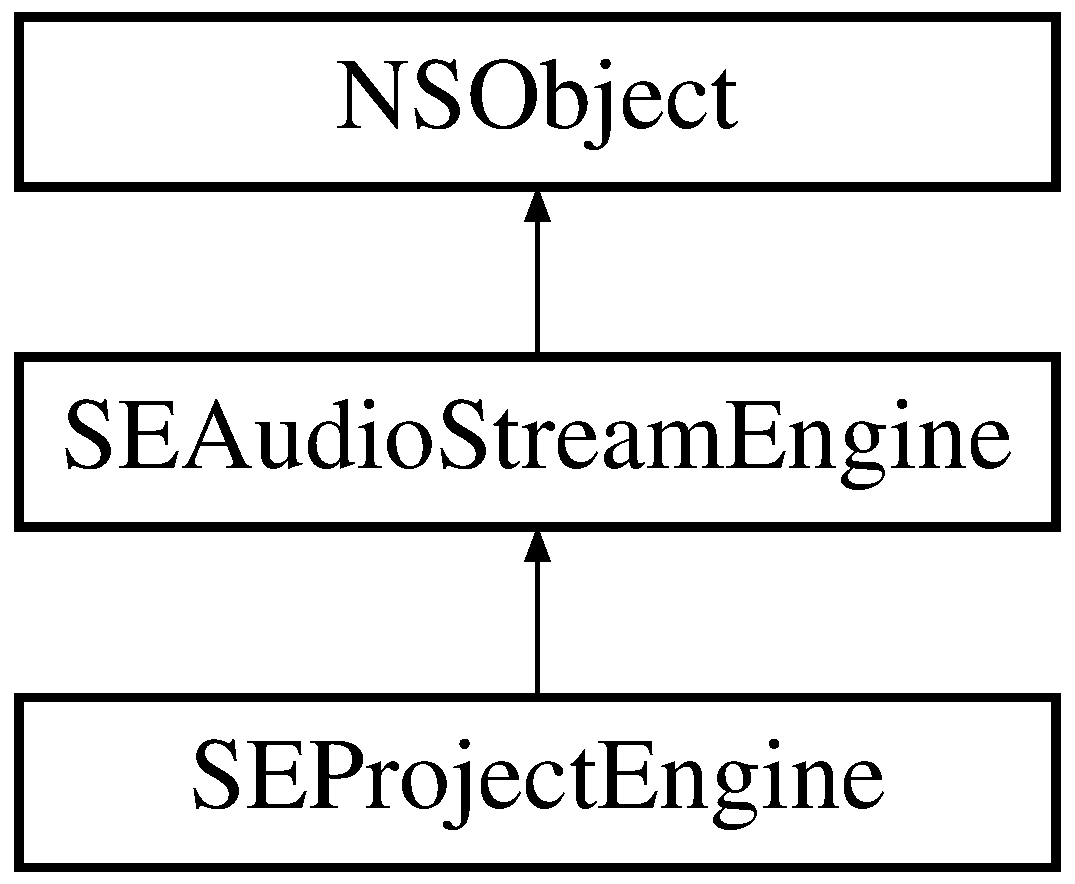
\includegraphics[height=3.000000cm]{interface_s_e_audio_stream_engine}
\end{center}
\end{figure}
\subsection*{Instance Methods}
\begin{DoxyCompactItemize}
\item 
(instancetype) -\/ \hyperlink{interface_s_e_audio_stream_engine_a1ec76b50caa6e569a74fb1fc642d6ede}{init\-With\-Stream\-:}
\item 
(void) -\/ \hyperlink{interface_s_e_audio_stream_engine_a6e3666a25828115786cc39ad40741a9d}{start\-Playing}
\item 
(void) -\/ \hyperlink{interface_s_e_audio_stream_engine_ae75c4a24cb45b92433a0f954c7180489}{pause\-Playing}
\item 
(void) -\/ \hyperlink{interface_s_e_audio_stream_engine_a77d1d55cf373ab32b01d20b7997b13f2}{stop\-Playing}
\item 
(void) -\/ \hyperlink{interface_s_e_audio_stream_engine_ad19a0488b4ea40ae9ae54c38526895de}{start\-Recording}
\item 
(void) -\/ \hyperlink{interface_s_e_audio_stream_engine_a2a1cd707ceb8fb2801826c38d932da66}{stop\-Recording}
\end{DoxyCompactItemize}
\subsection*{Properties}
\begin{DoxyCompactItemize}
\item 
id$<$ \hyperlink{protocol_s_e_audio_stream_engine_delegate-p}{S\-E\-Audio\-Stream\-Engine\-Delegate} $>$ \hyperlink{interface_s_e_audio_stream_engine_a83d462c8d145871aff485cc4dec5f9a5}{delegate}
\item 
\hyperlink{interface_s_e_audio_stream}{S\-E\-Audio\-Stream} $\ast$ \hyperlink{interface_s_e_audio_stream_engine_abe299880b85d0e7df2a9a2c6b6307dc3}{audio\-Stream}
\item 
\hyperlink{_s_e_audio_stream_engine_8h_a6eabe41a5616eddfad154f7259ccdc27}{T\-S\-E\-Audio\-Stream\-Engine\-State} \hyperlink{interface_s_e_audio_stream_engine_a124d47656b0b46ef4ec62ead90d17c47}{state}
\item 
N\-S\-Time\-Interval \hyperlink{interface_s_e_audio_stream_engine_ad7b5146644d4e96003f18756c4de975e}{current\-Time}
\item 
C\-G\-Float \hyperlink{interface_s_e_audio_stream_engine_aaddfc5a5f1cff2b0136665bc52e89ab1}{volume}
\item 
N\-S\-Time\-Interval \hyperlink{interface_s_e_audio_stream_engine_a9b03bb707f1b187e2d32e540f80a5dc1}{duration}
\item 
N\-S\-Error $\ast$ \hyperlink{interface_s_e_audio_stream_engine_a698b085efa2bb9de2fd2c24e98bf33cf}{error}
\end{DoxyCompactItemize}


\subsection{Method Documentation}
\hypertarget{interface_s_e_audio_stream_engine_a1ec76b50caa6e569a74fb1fc642d6ede}{\index{S\-E\-Audio\-Stream\-Engine@{S\-E\-Audio\-Stream\-Engine}!init\-With\-Stream\-:@{init\-With\-Stream\-:}}
\index{init\-With\-Stream\-:@{init\-With\-Stream\-:}!SEAudioStreamEngine@{S\-E\-Audio\-Stream\-Engine}}
\subsubsection[{init\-With\-Stream\-:}]{\setlength{\rightskip}{0pt plus 5cm}-\/ (instancetype) init\-With\-Stream\-: 
\begin{DoxyParamCaption}
\item[{({\bf S\-E\-Audio\-Stream}$\ast$)}]{stream}
\end{DoxyParamCaption}
}}\label{interface_s_e_audio_stream_engine_a1ec76b50caa6e569a74fb1fc642d6ede}
Load audio stream to player \hypertarget{interface_s_e_audio_stream_engine_ae75c4a24cb45b92433a0f954c7180489}{\index{S\-E\-Audio\-Stream\-Engine@{S\-E\-Audio\-Stream\-Engine}!pause\-Playing@{pause\-Playing}}
\index{pause\-Playing@{pause\-Playing}!SEAudioStreamEngine@{S\-E\-Audio\-Stream\-Engine}}
\subsubsection[{pause\-Playing}]{\setlength{\rightskip}{0pt plus 5cm}-\/ (void) pause\-Playing 
\begin{DoxyParamCaption}
{}
\end{DoxyParamCaption}
}}\label{interface_s_e_audio_stream_engine_ae75c4a24cb45b92433a0f954c7180489}
Pause on current position \hypertarget{interface_s_e_audio_stream_engine_a6e3666a25828115786cc39ad40741a9d}{\index{S\-E\-Audio\-Stream\-Engine@{S\-E\-Audio\-Stream\-Engine}!start\-Playing@{start\-Playing}}
\index{start\-Playing@{start\-Playing}!SEAudioStreamEngine@{S\-E\-Audio\-Stream\-Engine}}
\subsubsection[{start\-Playing}]{\setlength{\rightskip}{0pt plus 5cm}-\/ (void) start\-Playing 
\begin{DoxyParamCaption}
{}
\end{DoxyParamCaption}
}}\label{interface_s_e_audio_stream_engine_a6e3666a25828115786cc39ad40741a9d}
Start playing \hypertarget{interface_s_e_audio_stream_engine_ad19a0488b4ea40ae9ae54c38526895de}{\index{S\-E\-Audio\-Stream\-Engine@{S\-E\-Audio\-Stream\-Engine}!start\-Recording@{start\-Recording}}
\index{start\-Recording@{start\-Recording}!SEAudioStreamEngine@{S\-E\-Audio\-Stream\-Engine}}
\subsubsection[{start\-Recording}]{\setlength{\rightskip}{0pt plus 5cm}-\/ (void) start\-Recording 
\begin{DoxyParamCaption}
{}
\end{DoxyParamCaption}
}}\label{interface_s_e_audio_stream_engine_ad19a0488b4ea40ae9ae54c38526895de}
Start recording to stream \hypertarget{interface_s_e_audio_stream_engine_a77d1d55cf373ab32b01d20b7997b13f2}{\index{S\-E\-Audio\-Stream\-Engine@{S\-E\-Audio\-Stream\-Engine}!stop\-Playing@{stop\-Playing}}
\index{stop\-Playing@{stop\-Playing}!SEAudioStreamEngine@{S\-E\-Audio\-Stream\-Engine}}
\subsubsection[{stop\-Playing}]{\setlength{\rightskip}{0pt plus 5cm}-\/ (void) stop\-Playing 
\begin{DoxyParamCaption}
{}
\end{DoxyParamCaption}
}}\label{interface_s_e_audio_stream_engine_a77d1d55cf373ab32b01d20b7997b13f2}
Stop playing and seek to start \hypertarget{interface_s_e_audio_stream_engine_a2a1cd707ceb8fb2801826c38d932da66}{\index{S\-E\-Audio\-Stream\-Engine@{S\-E\-Audio\-Stream\-Engine}!stop\-Recording@{stop\-Recording}}
\index{stop\-Recording@{stop\-Recording}!SEAudioStreamEngine@{S\-E\-Audio\-Stream\-Engine}}
\subsubsection[{stop\-Recording}]{\setlength{\rightskip}{0pt plus 5cm}-\/ (void) stop\-Recording 
\begin{DoxyParamCaption}
{}
\end{DoxyParamCaption}
}}\label{interface_s_e_audio_stream_engine_a2a1cd707ceb8fb2801826c38d932da66}
Stop recording to stream 

\subsection{Property Documentation}
\hypertarget{interface_s_e_audio_stream_engine_abe299880b85d0e7df2a9a2c6b6307dc3}{\index{S\-E\-Audio\-Stream\-Engine@{S\-E\-Audio\-Stream\-Engine}!audio\-Stream@{audio\-Stream}}
\index{audio\-Stream@{audio\-Stream}!SEAudioStreamEngine@{S\-E\-Audio\-Stream\-Engine}}
\subsubsection[{audio\-Stream}]{\setlength{\rightskip}{0pt plus 5cm}-\/ ({\bf S\-E\-Audio\-Stream} $\ast$) audio\-Stream\hspace{0.3cm}{\ttfamily [read]}, {\ttfamily [nonatomic]}, {\ttfamily [assign]}}}\label{interface_s_e_audio_stream_engine_abe299880b85d0e7df2a9a2c6b6307dc3}
Pointer to stream \hypertarget{interface_s_e_audio_stream_engine_ad7b5146644d4e96003f18756c4de975e}{\index{S\-E\-Audio\-Stream\-Engine@{S\-E\-Audio\-Stream\-Engine}!current\-Time@{current\-Time}}
\index{current\-Time@{current\-Time}!SEAudioStreamEngine@{S\-E\-Audio\-Stream\-Engine}}
\subsubsection[{current\-Time}]{\setlength{\rightskip}{0pt plus 5cm}-\/ (N\-S\-Time\-Interval) current\-Time\hspace{0.3cm}{\ttfamily [read]}, {\ttfamily [write]}, {\ttfamily [nonatomic]}, {\ttfamily [assign]}}}\label{interface_s_e_audio_stream_engine_ad7b5146644d4e96003f18756c4de975e}
Current Time of audio track \hypertarget{interface_s_e_audio_stream_engine_a83d462c8d145871aff485cc4dec5f9a5}{\index{S\-E\-Audio\-Stream\-Engine@{S\-E\-Audio\-Stream\-Engine}!delegate@{delegate}}
\index{delegate@{delegate}!SEAudioStreamEngine@{S\-E\-Audio\-Stream\-Engine}}
\subsubsection[{delegate}]{\setlength{\rightskip}{0pt plus 5cm}-\/ (id$<${\bf S\-E\-Audio\-Stream\-Engine\-Delegate}$>$) delegate\hspace{0.3cm}{\ttfamily [read]}, {\ttfamily [write]}, {\ttfamily [nonatomic]}, {\ttfamily [weak]}}}\label{interface_s_e_audio_stream_engine_a83d462c8d145871aff485cc4dec5f9a5}
S\-E\-Audio\-Stream\-Player\-Delegate \hypertarget{interface_s_e_audio_stream_engine_a9b03bb707f1b187e2d32e540f80a5dc1}{\index{S\-E\-Audio\-Stream\-Engine@{S\-E\-Audio\-Stream\-Engine}!duration@{duration}}
\index{duration@{duration}!SEAudioStreamEngine@{S\-E\-Audio\-Stream\-Engine}}
\subsubsection[{duration}]{\setlength{\rightskip}{0pt plus 5cm}-\/ (N\-S\-Time\-Interval) duration\hspace{0.3cm}{\ttfamily [read]}, {\ttfamily [nonatomic]}, {\ttfamily [assign]}}}\label{interface_s_e_audio_stream_engine_a9b03bb707f1b187e2d32e540f80a5dc1}
Track duration \hypertarget{interface_s_e_audio_stream_engine_a698b085efa2bb9de2fd2c24e98bf33cf}{\index{S\-E\-Audio\-Stream\-Engine@{S\-E\-Audio\-Stream\-Engine}!error@{error}}
\index{error@{error}!SEAudioStreamEngine@{S\-E\-Audio\-Stream\-Engine}}
\subsubsection[{error}]{\setlength{\rightskip}{0pt plus 5cm}-\/ (N\-S\-Error $\ast$) error\hspace{0.3cm}{\ttfamily [read]}, {\ttfamily [nonatomic]}, {\ttfamily [assign]}}}\label{interface_s_e_audio_stream_engine_a698b085efa2bb9de2fd2c24e98bf33cf}
Last error \hypertarget{interface_s_e_audio_stream_engine_a124d47656b0b46ef4ec62ead90d17c47}{\index{S\-E\-Audio\-Stream\-Engine@{S\-E\-Audio\-Stream\-Engine}!state@{state}}
\index{state@{state}!SEAudioStreamEngine@{S\-E\-Audio\-Stream\-Engine}}
\subsubsection[{state}]{\setlength{\rightskip}{0pt plus 5cm}-\/ ({\bf T\-S\-E\-Audio\-Stream\-Engine\-State}) state\hspace{0.3cm}{\ttfamily [read]}, {\ttfamily [nonatomic]}, {\ttfamily [assign]}}}\label{interface_s_e_audio_stream_engine_a124d47656b0b46ef4ec62ead90d17c47}
State of engine \hypertarget{interface_s_e_audio_stream_engine_aaddfc5a5f1cff2b0136665bc52e89ab1}{\index{S\-E\-Audio\-Stream\-Engine@{S\-E\-Audio\-Stream\-Engine}!volume@{volume}}
\index{volume@{volume}!SEAudioStreamEngine@{S\-E\-Audio\-Stream\-Engine}}
\subsubsection[{volume}]{\setlength{\rightskip}{0pt plus 5cm}-\/ (C\-G\-Float) volume\hspace{0.3cm}{\ttfamily [read]}, {\ttfamily [write]}, {\ttfamily [nonatomic]}, {\ttfamily [assign]}}}\label{interface_s_e_audio_stream_engine_aaddfc5a5f1cff2b0136665bc52e89ab1}
Volume 0-\/1 

The documentation for this class was generated from the following files\-:\begin{DoxyCompactItemize}
\item 
/\-Users/igor/\-Develop/\-Develop\-Git/\-Davacon/i\-Phone/\-Sound\-Recorder/\-Classes/\-Core/\-Sound\-Editor/\hyperlink{_s_e_audio_stream_engine_8h}{S\-E\-Audio\-Stream\-Engine.\-h}\item 
/\-Users/igor/\-Develop/\-Develop\-Git/\-Davacon/i\-Phone/\-Sound\-Recorder/\-Classes/\-Core/\-Sound\-Editor/\hyperlink{_s_e_audio_stream_engine_8m}{S\-E\-Audio\-Stream\-Engine.\-m}\end{DoxyCompactItemize}

\hypertarget{category_s_e_audio_stream_engine_07_08}{\section{S\-E\-Audio\-Stream\-Engine() Category Reference}
\label{category_s_e_audio_stream_engine_07_08}\index{S\-E\-Audio\-Stream\-Engine()@{S\-E\-Audio\-Stream\-Engine()}}
}
\subsection*{Instance Methods}
\begin{DoxyCompactItemize}
\item 
(void) -\/ \hyperlink{category_s_e_audio_stream_engine_07_08_a904166440be2c605407aa2dfd37a8cec}{pm\-\_\-perform\-Error\-:}
\item 
(void) -\/ \hyperlink{category_s_e_audio_stream_engine_07_08_ac7baec71cdb25574abf73b975691d624}{pm\-\_\-process\-Output\-Buffer\-:queue\-:}
\item 
(void) -\/ \hyperlink{category_s_e_audio_stream_engine_07_08_adeb9a1148989f4bea42b99dfc7c24e34}{pm\-\_\-read\-Buffer\-Data\-With\-Duration\-:}
\item 
(int) -\/ \hyperlink{category_s_e_audio_stream_engine_07_08_a3f2ea6f72f3de68056d8b2a159e4b743}{pm\-\_\-compute\-Buffer\-Size\-With\-Format\-:seconds\-:}
\item 
(void) -\/ \hyperlink{category_s_e_audio_stream_engine_07_08_ad31ccee072ba39e61a59856ac4bb2c36}{pm\-\_\-process\-Input\-Buffer\-:queue\-:start\-Time\-:number\-Packet\-Descriptions\-:packet\-Descs\-:}
\item 
(void) -\/ \hyperlink{category_s_e_audio_stream_engine_07_08_a66b8ff5a0c4c3073c26122d247956abd}{pm\-\_\-on\-Play\-Timer}
\end{DoxyCompactItemize}
\subsection*{Properties}
\begin{DoxyCompactItemize}
\item 
\hyperlink{interface_s_e_audio_stream}{S\-E\-Audio\-Stream} $\ast$ \hyperlink{category_s_e_audio_stream_engine_07_08_ab9879d1cd039675a837837ccd094b956}{pv\-\_\-stream}
\item 
Audio\-Queue\-Ref \hyperlink{category_s_e_audio_stream_engine_07_08_aeba6c4680df8f38ea1271cfc52e697c5}{pv\-\_\-audio\-Output\-Queue}
\item 
Audio\-Queue\-Ref \hyperlink{category_s_e_audio_stream_engine_07_08_a4baace9b0ac0bccb1ab2e87446fb76be}{pv\-\_\-audio\-Input\-Queue}
\item 
N\-S\-U\-Integer \hyperlink{category_s_e_audio_stream_engine_07_08_a3248ba3a7ac29c4f865d24d084388ed0}{pv\-\_\-position}
\item 
N\-S\-Operation\-Queue $\ast$ \hyperlink{category_s_e_audio_stream_engine_07_08_adbcd5ee6428568c23a4a70a0387fe6bc}{pv\-\_\-queue}
\item 
\hyperlink{_s_e_audio_stream_engine_8h_a6eabe41a5616eddfad154f7259ccdc27}{T\-S\-E\-Audio\-Stream\-Engine\-State} \hyperlink{category_s_e_audio_stream_engine_07_08_a9f97a9d34b849921ab25f63422b4b02f}{pv\-\_\-state}
\item 
N\-S\-Error $\ast$ \hyperlink{category_s_e_audio_stream_engine_07_08_a553f6f36c7c69e5bcd7a63479b85c523}{pv\-\_\-error}
\item 
Audio\-Queue\-Buffer\-Ref \hyperlink{category_s_e_audio_stream_engine_07_08_ac0bed6a9ad4abf1fbaafc01fe2440283}{pv\-\_\-audio\-Buffer}
\item 
N\-S\-Mutable\-Data $\ast$ \hyperlink{category_s_e_audio_stream_engine_07_08_a358e58a2d9db7fd33050b6d3e3c00868}{pv\-\_\-play\-Buffer}
\item 
N\-S\-U\-Integer \hyperlink{category_s_e_audio_stream_engine_07_08_a357f65ae666f5971174ec6a162d76afd}{pv\-\_\-play\-Buffer\-Pos}
\item 
N\-S\-Timer $\ast$ \hyperlink{category_s_e_audio_stream_engine_07_08_aacc4ea3a3cebb5f53f99f8539e96b233}{pv\-\_\-play\-Timer}
\item 
B\-O\-O\-L \hyperlink{category_s_e_audio_stream_engine_07_08_a83ad29af81c705aa2f0f8474540f415e}{pv\-\_\-is\-Playing}
\end{DoxyCompactItemize}


\subsection{Method Documentation}
\hypertarget{category_s_e_audio_stream_engine_07_08_a3f2ea6f72f3de68056d8b2a159e4b743}{\index{S\-E\-Audio\-Stream\-Engine()@{S\-E\-Audio\-Stream\-Engine()}!pm\-\_\-compute\-Buffer\-Size\-With\-Format\-:seconds\-:@{pm\-\_\-compute\-Buffer\-Size\-With\-Format\-:seconds\-:}}
\index{pm\-\_\-compute\-Buffer\-Size\-With\-Format\-:seconds\-:@{pm\-\_\-compute\-Buffer\-Size\-With\-Format\-:seconds\-:}!SEAudioStreamEngine()@{S\-E\-Audio\-Stream\-Engine()}}
\subsubsection[{pm\-\_\-compute\-Buffer\-Size\-With\-Format\-:seconds\-:}]{\setlength{\rightskip}{0pt plus 5cm}-\/ (int) pm\-\_\-compute\-Buffer\-Size\-With\-Format\-: 
\begin{DoxyParamCaption}
\item[{(const Audio\-Stream\-Basic\-Description $\ast$)}]{format}
\item[{seconds:(float)}]{seconds}
\end{DoxyParamCaption}
}}\label{category_s_e_audio_stream_engine_07_08_a3f2ea6f72f3de68056d8b2a159e4b743}
\hypertarget{category_s_e_audio_stream_engine_07_08_a66b8ff5a0c4c3073c26122d247956abd}{\index{S\-E\-Audio\-Stream\-Engine()@{S\-E\-Audio\-Stream\-Engine()}!pm\-\_\-on\-Play\-Timer@{pm\-\_\-on\-Play\-Timer}}
\index{pm\-\_\-on\-Play\-Timer@{pm\-\_\-on\-Play\-Timer}!SEAudioStreamEngine()@{S\-E\-Audio\-Stream\-Engine()}}
\subsubsection[{pm\-\_\-on\-Play\-Timer}]{\setlength{\rightskip}{0pt plus 5cm}-\/ (void) pm\-\_\-on\-Play\-Timer 
\begin{DoxyParamCaption}
{}
\end{DoxyParamCaption}
}}\label{category_s_e_audio_stream_engine_07_08_a66b8ff5a0c4c3073c26122d247956abd}
\hypertarget{category_s_e_audio_stream_engine_07_08_a904166440be2c605407aa2dfd37a8cec}{\index{S\-E\-Audio\-Stream\-Engine()@{S\-E\-Audio\-Stream\-Engine()}!pm\-\_\-perform\-Error\-:@{pm\-\_\-perform\-Error\-:}}
\index{pm\-\_\-perform\-Error\-:@{pm\-\_\-perform\-Error\-:}!SEAudioStreamEngine()@{S\-E\-Audio\-Stream\-Engine()}}
\subsubsection[{pm\-\_\-perform\-Error\-:}]{\setlength{\rightskip}{0pt plus 5cm}-\/ (void) pm\-\_\-perform\-Error\-: 
\begin{DoxyParamCaption}
\item[{({\bf T\-S\-E\-Audio\-Stream\-Engine\-Error})}]{error\-Type}
\end{DoxyParamCaption}
}}\label{category_s_e_audio_stream_engine_07_08_a904166440be2c605407aa2dfd37a8cec}
\hypertarget{category_s_e_audio_stream_engine_07_08_ad31ccee072ba39e61a59856ac4bb2c36}{\index{S\-E\-Audio\-Stream\-Engine()@{S\-E\-Audio\-Stream\-Engine()}!pm\-\_\-process\-Input\-Buffer\-:queue\-:start\-Time\-:number\-Packet\-Descriptions\-:packet\-Descs\-:@{pm\-\_\-process\-Input\-Buffer\-:queue\-:start\-Time\-:number\-Packet\-Descriptions\-:packet\-Descs\-:}}
\index{pm\-\_\-process\-Input\-Buffer\-:queue\-:start\-Time\-:number\-Packet\-Descriptions\-:packet\-Descs\-:@{pm\-\_\-process\-Input\-Buffer\-:queue\-:start\-Time\-:number\-Packet\-Descriptions\-:packet\-Descs\-:}!SEAudioStreamEngine()@{S\-E\-Audio\-Stream\-Engine()}}
\subsubsection[{pm\-\_\-process\-Input\-Buffer\-:queue\-:start\-Time\-:number\-Packet\-Descriptions\-:packet\-Descs\-:}]{\setlength{\rightskip}{0pt plus 5cm}-\/ (void) pm\-\_\-process\-Input\-Buffer\-: 
\begin{DoxyParamCaption}
\item[{(Audio\-Queue\-Buffer\-Ref)}]{buffer}
\item[{queue:(Audio\-Queue\-Ref)}]{queue}
\item[{startTime:(const Audio\-Time\-Stamp $\ast$)}]{start\-Time}
\item[{numberPacketDescriptions:(U\-Int32)}]{in\-Number\-Packet\-Descriptions}
\item[{packetDescs:(const Audio\-Stream\-Packet\-Description $\ast$)}]{in\-Packet\-Descs}
\end{DoxyParamCaption}
}}\label{category_s_e_audio_stream_engine_07_08_ad31ccee072ba39e61a59856ac4bb2c36}
\hypertarget{category_s_e_audio_stream_engine_07_08_ac7baec71cdb25574abf73b975691d624}{\index{S\-E\-Audio\-Stream\-Engine()@{S\-E\-Audio\-Stream\-Engine()}!pm\-\_\-process\-Output\-Buffer\-:queue\-:@{pm\-\_\-process\-Output\-Buffer\-:queue\-:}}
\index{pm\-\_\-process\-Output\-Buffer\-:queue\-:@{pm\-\_\-process\-Output\-Buffer\-:queue\-:}!SEAudioStreamEngine()@{S\-E\-Audio\-Stream\-Engine()}}
\subsubsection[{pm\-\_\-process\-Output\-Buffer\-:queue\-:}]{\setlength{\rightskip}{0pt plus 5cm}-\/ (void) pm\-\_\-process\-Output\-Buffer\-: 
\begin{DoxyParamCaption}
\item[{(Audio\-Queue\-Buffer\-Ref)}]{buffer}
\item[{queue:(Audio\-Queue\-Ref)}]{queue}
\end{DoxyParamCaption}
}}\label{category_s_e_audio_stream_engine_07_08_ac7baec71cdb25574abf73b975691d624}
\hypertarget{category_s_e_audio_stream_engine_07_08_adeb9a1148989f4bea42b99dfc7c24e34}{\index{S\-E\-Audio\-Stream\-Engine()@{S\-E\-Audio\-Stream\-Engine()}!pm\-\_\-read\-Buffer\-Data\-With\-Duration\-:@{pm\-\_\-read\-Buffer\-Data\-With\-Duration\-:}}
\index{pm\-\_\-read\-Buffer\-Data\-With\-Duration\-:@{pm\-\_\-read\-Buffer\-Data\-With\-Duration\-:}!SEAudioStreamEngine()@{S\-E\-Audio\-Stream\-Engine()}}
\subsubsection[{pm\-\_\-read\-Buffer\-Data\-With\-Duration\-:}]{\setlength{\rightskip}{0pt plus 5cm}-\/ (void) pm\-\_\-read\-Buffer\-Data\-With\-Duration\-: 
\begin{DoxyParamCaption}
\item[{(N\-S\-U\-Integer)}]{duration}
\end{DoxyParamCaption}
}}\label{category_s_e_audio_stream_engine_07_08_adeb9a1148989f4bea42b99dfc7c24e34}


\subsection{Property Documentation}
\hypertarget{category_s_e_audio_stream_engine_07_08_ac0bed6a9ad4abf1fbaafc01fe2440283}{\index{S\-E\-Audio\-Stream\-Engine()@{S\-E\-Audio\-Stream\-Engine()}!pv\-\_\-audio\-Buffer@{pv\-\_\-audio\-Buffer}}
\index{pv\-\_\-audio\-Buffer@{pv\-\_\-audio\-Buffer}!SEAudioStreamEngine()@{S\-E\-Audio\-Stream\-Engine()}}
\subsubsection[{pv\-\_\-audio\-Buffer}]{\setlength{\rightskip}{0pt plus 5cm}-\/ (Audio\-Queue\-Buffer\-Ref) pv\-\_\-audio\-Buffer\hspace{0.3cm}{\ttfamily [read]}, {\ttfamily [write]}, {\ttfamily [nonatomic]}, {\ttfamily [assign]}}}\label{category_s_e_audio_stream_engine_07_08_ac0bed6a9ad4abf1fbaafc01fe2440283}
\hypertarget{category_s_e_audio_stream_engine_07_08_a4baace9b0ac0bccb1ab2e87446fb76be}{\index{S\-E\-Audio\-Stream\-Engine()@{S\-E\-Audio\-Stream\-Engine()}!pv\-\_\-audio\-Input\-Queue@{pv\-\_\-audio\-Input\-Queue}}
\index{pv\-\_\-audio\-Input\-Queue@{pv\-\_\-audio\-Input\-Queue}!SEAudioStreamEngine()@{S\-E\-Audio\-Stream\-Engine()}}
\subsubsection[{pv\-\_\-audio\-Input\-Queue}]{\setlength{\rightskip}{0pt plus 5cm}-\/ (Audio\-Queue\-Ref) pv\-\_\-audio\-Input\-Queue\hspace{0.3cm}{\ttfamily [read]}, {\ttfamily [write]}, {\ttfamily [nonatomic]}, {\ttfamily [assign]}}}\label{category_s_e_audio_stream_engine_07_08_a4baace9b0ac0bccb1ab2e87446fb76be}
\hypertarget{category_s_e_audio_stream_engine_07_08_aeba6c4680df8f38ea1271cfc52e697c5}{\index{S\-E\-Audio\-Stream\-Engine()@{S\-E\-Audio\-Stream\-Engine()}!pv\-\_\-audio\-Output\-Queue@{pv\-\_\-audio\-Output\-Queue}}
\index{pv\-\_\-audio\-Output\-Queue@{pv\-\_\-audio\-Output\-Queue}!SEAudioStreamEngine()@{S\-E\-Audio\-Stream\-Engine()}}
\subsubsection[{pv\-\_\-audio\-Output\-Queue}]{\setlength{\rightskip}{0pt plus 5cm}-\/ (Audio\-Queue\-Ref) pv\-\_\-audio\-Output\-Queue\hspace{0.3cm}{\ttfamily [read]}, {\ttfamily [write]}, {\ttfamily [nonatomic]}, {\ttfamily [assign]}}}\label{category_s_e_audio_stream_engine_07_08_aeba6c4680df8f38ea1271cfc52e697c5}
\hypertarget{category_s_e_audio_stream_engine_07_08_a553f6f36c7c69e5bcd7a63479b85c523}{\index{S\-E\-Audio\-Stream\-Engine()@{S\-E\-Audio\-Stream\-Engine()}!pv\-\_\-error@{pv\-\_\-error}}
\index{pv\-\_\-error@{pv\-\_\-error}!SEAudioStreamEngine()@{S\-E\-Audio\-Stream\-Engine()}}
\subsubsection[{pv\-\_\-error}]{\setlength{\rightskip}{0pt plus 5cm}-\/ (N\-S\-Error$\ast$) pv\-\_\-error\hspace{0.3cm}{\ttfamily [read]}, {\ttfamily [write]}, {\ttfamily [nonatomic]}, {\ttfamily [strong]}}}\label{category_s_e_audio_stream_engine_07_08_a553f6f36c7c69e5bcd7a63479b85c523}
\hypertarget{category_s_e_audio_stream_engine_07_08_a83ad29af81c705aa2f0f8474540f415e}{\index{S\-E\-Audio\-Stream\-Engine()@{S\-E\-Audio\-Stream\-Engine()}!pv\-\_\-is\-Playing@{pv\-\_\-is\-Playing}}
\index{pv\-\_\-is\-Playing@{pv\-\_\-is\-Playing}!SEAudioStreamEngine()@{S\-E\-Audio\-Stream\-Engine()}}
\subsubsection[{pv\-\_\-is\-Playing}]{\setlength{\rightskip}{0pt plus 5cm}-\/ (B\-O\-O\-L) pv\-\_\-is\-Playing\hspace{0.3cm}{\ttfamily [read]}, {\ttfamily [write]}, {\ttfamily [nonatomic]}, {\ttfamily [assign]}}}\label{category_s_e_audio_stream_engine_07_08_a83ad29af81c705aa2f0f8474540f415e}
\hypertarget{category_s_e_audio_stream_engine_07_08_a358e58a2d9db7fd33050b6d3e3c00868}{\index{S\-E\-Audio\-Stream\-Engine()@{S\-E\-Audio\-Stream\-Engine()}!pv\-\_\-play\-Buffer@{pv\-\_\-play\-Buffer}}
\index{pv\-\_\-play\-Buffer@{pv\-\_\-play\-Buffer}!SEAudioStreamEngine()@{S\-E\-Audio\-Stream\-Engine()}}
\subsubsection[{pv\-\_\-play\-Buffer}]{\setlength{\rightskip}{0pt plus 5cm}-\/ (N\-S\-Mutable\-Data$\ast$) pv\-\_\-play\-Buffer\hspace{0.3cm}{\ttfamily [read]}, {\ttfamily [write]}, {\ttfamily [nonatomic]}, {\ttfamily [strong]}}}\label{category_s_e_audio_stream_engine_07_08_a358e58a2d9db7fd33050b6d3e3c00868}
\hypertarget{category_s_e_audio_stream_engine_07_08_a357f65ae666f5971174ec6a162d76afd}{\index{S\-E\-Audio\-Stream\-Engine()@{S\-E\-Audio\-Stream\-Engine()}!pv\-\_\-play\-Buffer\-Pos@{pv\-\_\-play\-Buffer\-Pos}}
\index{pv\-\_\-play\-Buffer\-Pos@{pv\-\_\-play\-Buffer\-Pos}!SEAudioStreamEngine()@{S\-E\-Audio\-Stream\-Engine()}}
\subsubsection[{pv\-\_\-play\-Buffer\-Pos}]{\setlength{\rightskip}{0pt plus 5cm}-\/ (N\-S\-U\-Integer) pv\-\_\-play\-Buffer\-Pos\hspace{0.3cm}{\ttfamily [read]}, {\ttfamily [write]}, {\ttfamily [nonatomic]}, {\ttfamily [assign]}}}\label{category_s_e_audio_stream_engine_07_08_a357f65ae666f5971174ec6a162d76afd}
\hypertarget{category_s_e_audio_stream_engine_07_08_aacc4ea3a3cebb5f53f99f8539e96b233}{\index{S\-E\-Audio\-Stream\-Engine()@{S\-E\-Audio\-Stream\-Engine()}!pv\-\_\-play\-Timer@{pv\-\_\-play\-Timer}}
\index{pv\-\_\-play\-Timer@{pv\-\_\-play\-Timer}!SEAudioStreamEngine()@{S\-E\-Audio\-Stream\-Engine()}}
\subsubsection[{pv\-\_\-play\-Timer}]{\setlength{\rightskip}{0pt plus 5cm}-\/ (N\-S\-Timer$\ast$) pv\-\_\-play\-Timer\hspace{0.3cm}{\ttfamily [read]}, {\ttfamily [write]}, {\ttfamily [nonatomic]}, {\ttfamily [strong]}}}\label{category_s_e_audio_stream_engine_07_08_aacc4ea3a3cebb5f53f99f8539e96b233}
\hypertarget{category_s_e_audio_stream_engine_07_08_a3248ba3a7ac29c4f865d24d084388ed0}{\index{S\-E\-Audio\-Stream\-Engine()@{S\-E\-Audio\-Stream\-Engine()}!pv\-\_\-position@{pv\-\_\-position}}
\index{pv\-\_\-position@{pv\-\_\-position}!SEAudioStreamEngine()@{S\-E\-Audio\-Stream\-Engine()}}
\subsubsection[{pv\-\_\-position}]{\setlength{\rightskip}{0pt plus 5cm}-\/ (N\-S\-U\-Integer) pv\-\_\-position\hspace{0.3cm}{\ttfamily [read]}, {\ttfamily [write]}, {\ttfamily [nonatomic]}, {\ttfamily [assign]}}}\label{category_s_e_audio_stream_engine_07_08_a3248ba3a7ac29c4f865d24d084388ed0}
\hypertarget{category_s_e_audio_stream_engine_07_08_adbcd5ee6428568c23a4a70a0387fe6bc}{\index{S\-E\-Audio\-Stream\-Engine()@{S\-E\-Audio\-Stream\-Engine()}!pv\-\_\-queue@{pv\-\_\-queue}}
\index{pv\-\_\-queue@{pv\-\_\-queue}!SEAudioStreamEngine()@{S\-E\-Audio\-Stream\-Engine()}}
\subsubsection[{pv\-\_\-queue}]{\setlength{\rightskip}{0pt plus 5cm}-\/ (N\-S\-Operation\-Queue$\ast$) pv\-\_\-queue\hspace{0.3cm}{\ttfamily [read]}, {\ttfamily [write]}, {\ttfamily [nonatomic]}, {\ttfamily [strong]}}}\label{category_s_e_audio_stream_engine_07_08_adbcd5ee6428568c23a4a70a0387fe6bc}
\hypertarget{category_s_e_audio_stream_engine_07_08_a9f97a9d34b849921ab25f63422b4b02f}{\index{S\-E\-Audio\-Stream\-Engine()@{S\-E\-Audio\-Stream\-Engine()}!pv\-\_\-state@{pv\-\_\-state}}
\index{pv\-\_\-state@{pv\-\_\-state}!SEAudioStreamEngine()@{S\-E\-Audio\-Stream\-Engine()}}
\subsubsection[{pv\-\_\-state}]{\setlength{\rightskip}{0pt plus 5cm}-\/ ({\bf T\-S\-E\-Audio\-Stream\-Engine\-State}) pv\-\_\-state\hspace{0.3cm}{\ttfamily [read]}, {\ttfamily [write]}, {\ttfamily [nonatomic]}, {\ttfamily [assign]}}}\label{category_s_e_audio_stream_engine_07_08_a9f97a9d34b849921ab25f63422b4b02f}
\hypertarget{category_s_e_audio_stream_engine_07_08_ab9879d1cd039675a837837ccd094b956}{\index{S\-E\-Audio\-Stream\-Engine()@{S\-E\-Audio\-Stream\-Engine()}!pv\-\_\-stream@{pv\-\_\-stream}}
\index{pv\-\_\-stream@{pv\-\_\-stream}!SEAudioStreamEngine()@{S\-E\-Audio\-Stream\-Engine()}}
\subsubsection[{pv\-\_\-stream}]{\setlength{\rightskip}{0pt plus 5cm}-\/ ({\bf S\-E\-Audio\-Stream}$\ast$) pv\-\_\-stream\hspace{0.3cm}{\ttfamily [read]}, {\ttfamily [write]}, {\ttfamily [nonatomic]}, {\ttfamily [strong]}}}\label{category_s_e_audio_stream_engine_07_08_ab9879d1cd039675a837837ccd094b956}


The documentation for this category was generated from the following file\-:\begin{DoxyCompactItemize}
\item 
/\-Users/igor/\-Develop/\-Develop\-Git/\-Davacon/i\-Phone/\-Sound\-Recorder/\-Classes/\-Core/\-Sound\-Editor/\hyperlink{_s_e_audio_stream_engine_8m}{S\-E\-Audio\-Stream\-Engine.\-m}\end{DoxyCompactItemize}

\hypertarget{protocol_s_e_audio_stream_engine_delegate-p}{\section{$<$S\-E\-Audio\-Stream\-Engine\-Delegate$>$ Protocol Reference}
\label{protocol_s_e_audio_stream_engine_delegate-p}\index{$<$\-S\-E\-Audio\-Stream\-Engine\-Delegate$>$@{$<$\-S\-E\-Audio\-Stream\-Engine\-Delegate$>$}}
}


{\ttfamily \#import $<$S\-E\-Audio\-Stream\-Engine.\-h$>$}

Inheritance diagram for $<$S\-E\-Audio\-Stream\-Engine\-Delegate$>$\-:\begin{figure}[H]
\begin{center}
\leavevmode
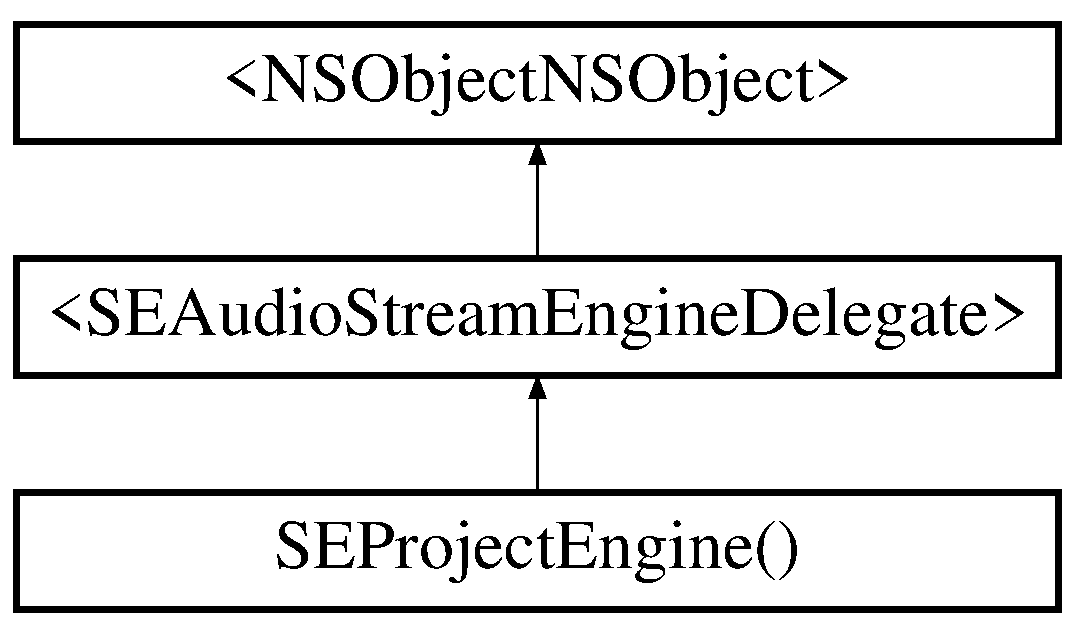
\includegraphics[height=3.000000cm]{protocol_s_e_audio_stream_engine_delegate-p}
\end{center}
\end{figure}
\subsection*{Instance Methods}
\begin{DoxyCompactItemize}
\item 
(void) -\/ \hyperlink{protocol_s_e_audio_stream_engine_delegate-p_ad028df707bf49e8666b815bde8f40902}{audio\-Stream\-Engine\-Did\-Start\-Playing\-:}
\item 
(void) -\/ \hyperlink{protocol_s_e_audio_stream_engine_delegate-p_a1bd5a2cc2a8c641534cbb74a55773fcb}{audio\-Stream\-Engine\-Did\-Pause\-:}
\item 
(void) -\/ \hyperlink{protocol_s_e_audio_stream_engine_delegate-p_a25a68e34ad837b70cedc6d8485185fe3}{audio\-Stream\-Engine\-Did\-Continue\-:}
\item 
(void) -\/ \hyperlink{protocol_s_e_audio_stream_engine_delegate-p_af917adce2406d3802da99282c8fc1723}{audio\-Stream\-Engine\-Playing\-:did\-Update\-With\-Current\-Time\-:}
\item 
(void) -\/ \hyperlink{protocol_s_e_audio_stream_engine_delegate-p_a824aeca3299956565bfaa84ba4d04f33}{audio\-Stream\-Engine\-Did\-Finish\-Playing\-:stopped\-:}
\item 
(void) -\/ \hyperlink{protocol_s_e_audio_stream_engine_delegate-p_a192f31070f458201190d97c2e3dbbbee}{audio\-Stream\-Engine\-Did\-Start\-Recording\-:}
\item 
(void) -\/ \hyperlink{protocol_s_e_audio_stream_engine_delegate-p_a75f167807ad628680176d4438aeb840a}{audio\-Stream\-Engine\-Recording\-:did\-Update\-With\-Current\-Time\-:}
\item 
(void) -\/ \hyperlink{protocol_s_e_audio_stream_engine_delegate-p_ad693afa65ce5cc6560f40b8cf9719606}{audio\-Stream\-Engine\-Did\-Stop\-Recording\-:}
\item 
(void) -\/ \hyperlink{protocol_s_e_audio_stream_engine_delegate-p_afbb8aa7876ff176dc2e3bf52343084ce}{audio\-Stream\-Engine\-:did\-Occur\-Error\-:}
\end{DoxyCompactItemize}


\subsection{Method Documentation}
\hypertarget{protocol_s_e_audio_stream_engine_delegate-p_afbb8aa7876ff176dc2e3bf52343084ce}{\index{S\-E\-Audio\-Stream\-Engine\-Delegate-\/p@{S\-E\-Audio\-Stream\-Engine\-Delegate-\/p}!audio\-Stream\-Engine\-:did\-Occur\-Error\-:@{audio\-Stream\-Engine\-:did\-Occur\-Error\-:}}
\index{audio\-Stream\-Engine\-:did\-Occur\-Error\-:@{audio\-Stream\-Engine\-:did\-Occur\-Error\-:}!SEAudioStreamEngineDelegate-p@{S\-E\-Audio\-Stream\-Engine\-Delegate-\/p}}
\subsubsection[{audio\-Stream\-Engine\-:did\-Occur\-Error\-:}]{\setlength{\rightskip}{0pt plus 5cm}-\/ (void) audio\-Stream\-Engine\-: 
\begin{DoxyParamCaption}
\item[{({\bf S\-E\-Audio\-Stream\-Engine} $\ast$)}]{engine}
\item[{didOccurError:(N\-S\-Error $\ast$)}]{error}
\end{DoxyParamCaption}
\hspace{0.3cm}{\ttfamily [optional]}}}\label{protocol_s_e_audio_stream_engine_delegate-p_afbb8aa7876ff176dc2e3bf52343084ce}
Notification for error \hypertarget{protocol_s_e_audio_stream_engine_delegate-p_a25a68e34ad837b70cedc6d8485185fe3}{\index{S\-E\-Audio\-Stream\-Engine\-Delegate-\/p@{S\-E\-Audio\-Stream\-Engine\-Delegate-\/p}!audio\-Stream\-Engine\-Did\-Continue\-:@{audio\-Stream\-Engine\-Did\-Continue\-:}}
\index{audio\-Stream\-Engine\-Did\-Continue\-:@{audio\-Stream\-Engine\-Did\-Continue\-:}!SEAudioStreamEngineDelegate-p@{S\-E\-Audio\-Stream\-Engine\-Delegate-\/p}}
\subsubsection[{audio\-Stream\-Engine\-Did\-Continue\-:}]{\setlength{\rightskip}{0pt plus 5cm}-\/ (void) audio\-Stream\-Engine\-Did\-Continue\-: 
\begin{DoxyParamCaption}
\item[{({\bf S\-E\-Audio\-Stream\-Engine} $\ast$)}]{engine}
\end{DoxyParamCaption}
\hspace{0.3cm}{\ttfamily [optional]}}}\label{protocol_s_e_audio_stream_engine_delegate-p_a25a68e34ad837b70cedc6d8485185fe3}
Notification for continue playing after pause \hypertarget{protocol_s_e_audio_stream_engine_delegate-p_a824aeca3299956565bfaa84ba4d04f33}{\index{S\-E\-Audio\-Stream\-Engine\-Delegate-\/p@{S\-E\-Audio\-Stream\-Engine\-Delegate-\/p}!audio\-Stream\-Engine\-Did\-Finish\-Playing\-:stopped\-:@{audio\-Stream\-Engine\-Did\-Finish\-Playing\-:stopped\-:}}
\index{audio\-Stream\-Engine\-Did\-Finish\-Playing\-:stopped\-:@{audio\-Stream\-Engine\-Did\-Finish\-Playing\-:stopped\-:}!SEAudioStreamEngineDelegate-p@{S\-E\-Audio\-Stream\-Engine\-Delegate-\/p}}
\subsubsection[{audio\-Stream\-Engine\-Did\-Finish\-Playing\-:stopped\-:}]{\setlength{\rightskip}{0pt plus 5cm}-\/ (void) audio\-Stream\-Engine\-Did\-Finish\-Playing\-: 
\begin{DoxyParamCaption}
\item[{({\bf S\-E\-Audio\-Stream\-Engine} $\ast$)}]{engine}
\item[{stopped:(B\-O\-O\-L)}]{stopped}
\end{DoxyParamCaption}
\hspace{0.3cm}{\ttfamily [optional]}}}\label{protocol_s_e_audio_stream_engine_delegate-p_a824aeca3299956565bfaa84ba4d04f33}
Notification for end playing \hypertarget{protocol_s_e_audio_stream_engine_delegate-p_a1bd5a2cc2a8c641534cbb74a55773fcb}{\index{S\-E\-Audio\-Stream\-Engine\-Delegate-\/p@{S\-E\-Audio\-Stream\-Engine\-Delegate-\/p}!audio\-Stream\-Engine\-Did\-Pause\-:@{audio\-Stream\-Engine\-Did\-Pause\-:}}
\index{audio\-Stream\-Engine\-Did\-Pause\-:@{audio\-Stream\-Engine\-Did\-Pause\-:}!SEAudioStreamEngineDelegate-p@{S\-E\-Audio\-Stream\-Engine\-Delegate-\/p}}
\subsubsection[{audio\-Stream\-Engine\-Did\-Pause\-:}]{\setlength{\rightskip}{0pt plus 5cm}-\/ (void) audio\-Stream\-Engine\-Did\-Pause\-: 
\begin{DoxyParamCaption}
\item[{({\bf S\-E\-Audio\-Stream\-Engine} $\ast$)}]{engine}
\end{DoxyParamCaption}
\hspace{0.3cm}{\ttfamily [optional]}}}\label{protocol_s_e_audio_stream_engine_delegate-p_a1bd5a2cc2a8c641534cbb74a55773fcb}
Notification for pause playing \hypertarget{protocol_s_e_audio_stream_engine_delegate-p_ad028df707bf49e8666b815bde8f40902}{\index{S\-E\-Audio\-Stream\-Engine\-Delegate-\/p@{S\-E\-Audio\-Stream\-Engine\-Delegate-\/p}!audio\-Stream\-Engine\-Did\-Start\-Playing\-:@{audio\-Stream\-Engine\-Did\-Start\-Playing\-:}}
\index{audio\-Stream\-Engine\-Did\-Start\-Playing\-:@{audio\-Stream\-Engine\-Did\-Start\-Playing\-:}!SEAudioStreamEngineDelegate-p@{S\-E\-Audio\-Stream\-Engine\-Delegate-\/p}}
\subsubsection[{audio\-Stream\-Engine\-Did\-Start\-Playing\-:}]{\setlength{\rightskip}{0pt plus 5cm}-\/ (void) audio\-Stream\-Engine\-Did\-Start\-Playing\-: 
\begin{DoxyParamCaption}
\item[{({\bf S\-E\-Audio\-Stream\-Engine} $\ast$)}]{engine}
\end{DoxyParamCaption}
\hspace{0.3cm}{\ttfamily [optional]}}}\label{protocol_s_e_audio_stream_engine_delegate-p_ad028df707bf49e8666b815bde8f40902}
Notification for begin playing \hypertarget{protocol_s_e_audio_stream_engine_delegate-p_a192f31070f458201190d97c2e3dbbbee}{\index{S\-E\-Audio\-Stream\-Engine\-Delegate-\/p@{S\-E\-Audio\-Stream\-Engine\-Delegate-\/p}!audio\-Stream\-Engine\-Did\-Start\-Recording\-:@{audio\-Stream\-Engine\-Did\-Start\-Recording\-:}}
\index{audio\-Stream\-Engine\-Did\-Start\-Recording\-:@{audio\-Stream\-Engine\-Did\-Start\-Recording\-:}!SEAudioStreamEngineDelegate-p@{S\-E\-Audio\-Stream\-Engine\-Delegate-\/p}}
\subsubsection[{audio\-Stream\-Engine\-Did\-Start\-Recording\-:}]{\setlength{\rightskip}{0pt plus 5cm}-\/ (void) audio\-Stream\-Engine\-Did\-Start\-Recording\-: 
\begin{DoxyParamCaption}
\item[{({\bf S\-E\-Audio\-Stream\-Engine} $\ast$)}]{engine}
\end{DoxyParamCaption}
\hspace{0.3cm}{\ttfamily [optional]}}}\label{protocol_s_e_audio_stream_engine_delegate-p_a192f31070f458201190d97c2e3dbbbee}
Notification for start recording \hypertarget{protocol_s_e_audio_stream_engine_delegate-p_ad693afa65ce5cc6560f40b8cf9719606}{\index{S\-E\-Audio\-Stream\-Engine\-Delegate-\/p@{S\-E\-Audio\-Stream\-Engine\-Delegate-\/p}!audio\-Stream\-Engine\-Did\-Stop\-Recording\-:@{audio\-Stream\-Engine\-Did\-Stop\-Recording\-:}}
\index{audio\-Stream\-Engine\-Did\-Stop\-Recording\-:@{audio\-Stream\-Engine\-Did\-Stop\-Recording\-:}!SEAudioStreamEngineDelegate-p@{S\-E\-Audio\-Stream\-Engine\-Delegate-\/p}}
\subsubsection[{audio\-Stream\-Engine\-Did\-Stop\-Recording\-:}]{\setlength{\rightskip}{0pt plus 5cm}-\/ (void) audio\-Stream\-Engine\-Did\-Stop\-Recording\-: 
\begin{DoxyParamCaption}
\item[{({\bf S\-E\-Audio\-Stream\-Engine} $\ast$)}]{engine}
\end{DoxyParamCaption}
\hspace{0.3cm}{\ttfamily [optional]}}}\label{protocol_s_e_audio_stream_engine_delegate-p_ad693afa65ce5cc6560f40b8cf9719606}
Notification for end recording \hypertarget{protocol_s_e_audio_stream_engine_delegate-p_af917adce2406d3802da99282c8fc1723}{\index{S\-E\-Audio\-Stream\-Engine\-Delegate-\/p@{S\-E\-Audio\-Stream\-Engine\-Delegate-\/p}!audio\-Stream\-Engine\-Playing\-:did\-Update\-With\-Current\-Time\-:@{audio\-Stream\-Engine\-Playing\-:did\-Update\-With\-Current\-Time\-:}}
\index{audio\-Stream\-Engine\-Playing\-:did\-Update\-With\-Current\-Time\-:@{audio\-Stream\-Engine\-Playing\-:did\-Update\-With\-Current\-Time\-:}!SEAudioStreamEngineDelegate-p@{S\-E\-Audio\-Stream\-Engine\-Delegate-\/p}}
\subsubsection[{audio\-Stream\-Engine\-Playing\-:did\-Update\-With\-Current\-Time\-:}]{\setlength{\rightskip}{0pt plus 5cm}-\/ (void) audio\-Stream\-Engine\-Playing\-: 
\begin{DoxyParamCaption}
\item[{({\bf S\-E\-Audio\-Stream\-Engine} $\ast$)}]{engine}
\item[{didUpdateWithCurrentTime:(N\-S\-Time\-Interval)}]{time}
\end{DoxyParamCaption}
\hspace{0.3cm}{\ttfamily [optional]}}}\label{protocol_s_e_audio_stream_engine_delegate-p_af917adce2406d3802da99282c8fc1723}
Notification for updating info about play state \hypertarget{protocol_s_e_audio_stream_engine_delegate-p_a75f167807ad628680176d4438aeb840a}{\index{S\-E\-Audio\-Stream\-Engine\-Delegate-\/p@{S\-E\-Audio\-Stream\-Engine\-Delegate-\/p}!audio\-Stream\-Engine\-Recording\-:did\-Update\-With\-Current\-Time\-:@{audio\-Stream\-Engine\-Recording\-:did\-Update\-With\-Current\-Time\-:}}
\index{audio\-Stream\-Engine\-Recording\-:did\-Update\-With\-Current\-Time\-:@{audio\-Stream\-Engine\-Recording\-:did\-Update\-With\-Current\-Time\-:}!SEAudioStreamEngineDelegate-p@{S\-E\-Audio\-Stream\-Engine\-Delegate-\/p}}
\subsubsection[{audio\-Stream\-Engine\-Recording\-:did\-Update\-With\-Current\-Time\-:}]{\setlength{\rightskip}{0pt plus 5cm}-\/ (void) audio\-Stream\-Engine\-Recording\-: 
\begin{DoxyParamCaption}
\item[{({\bf S\-E\-Audio\-Stream\-Engine} $\ast$)}]{engine}
\item[{didUpdateWithCurrentTime:(N\-S\-Time\-Interval)}]{time}
\end{DoxyParamCaption}
\hspace{0.3cm}{\ttfamily [optional]}}}\label{protocol_s_e_audio_stream_engine_delegate-p_a75f167807ad628680176d4438aeb840a}
Notification for updating info about play state 

The documentation for this protocol was generated from the following file\-:\begin{DoxyCompactItemize}
\item 
/\-Users/igor/\-Develop/\-Develop\-Git/\-Davacon/i\-Phone/\-Sound\-Recorder/\-Classes/\-Core/\-Sound\-Editor/\hyperlink{_s_e_audio_stream_engine_8h}{S\-E\-Audio\-Stream\-Engine.\-h}\end{DoxyCompactItemize}

\hypertarget{interface_s_e_project}{\section{S\-E\-Project Class Reference}
\label{interface_s_e_project}\index{S\-E\-Project@{S\-E\-Project}}
}


{\ttfamily \#import $<$S\-E\-Project.\-h$>$}

Inheritance diagram for S\-E\-Project\-:\begin{figure}[H]
\begin{center}
\leavevmode
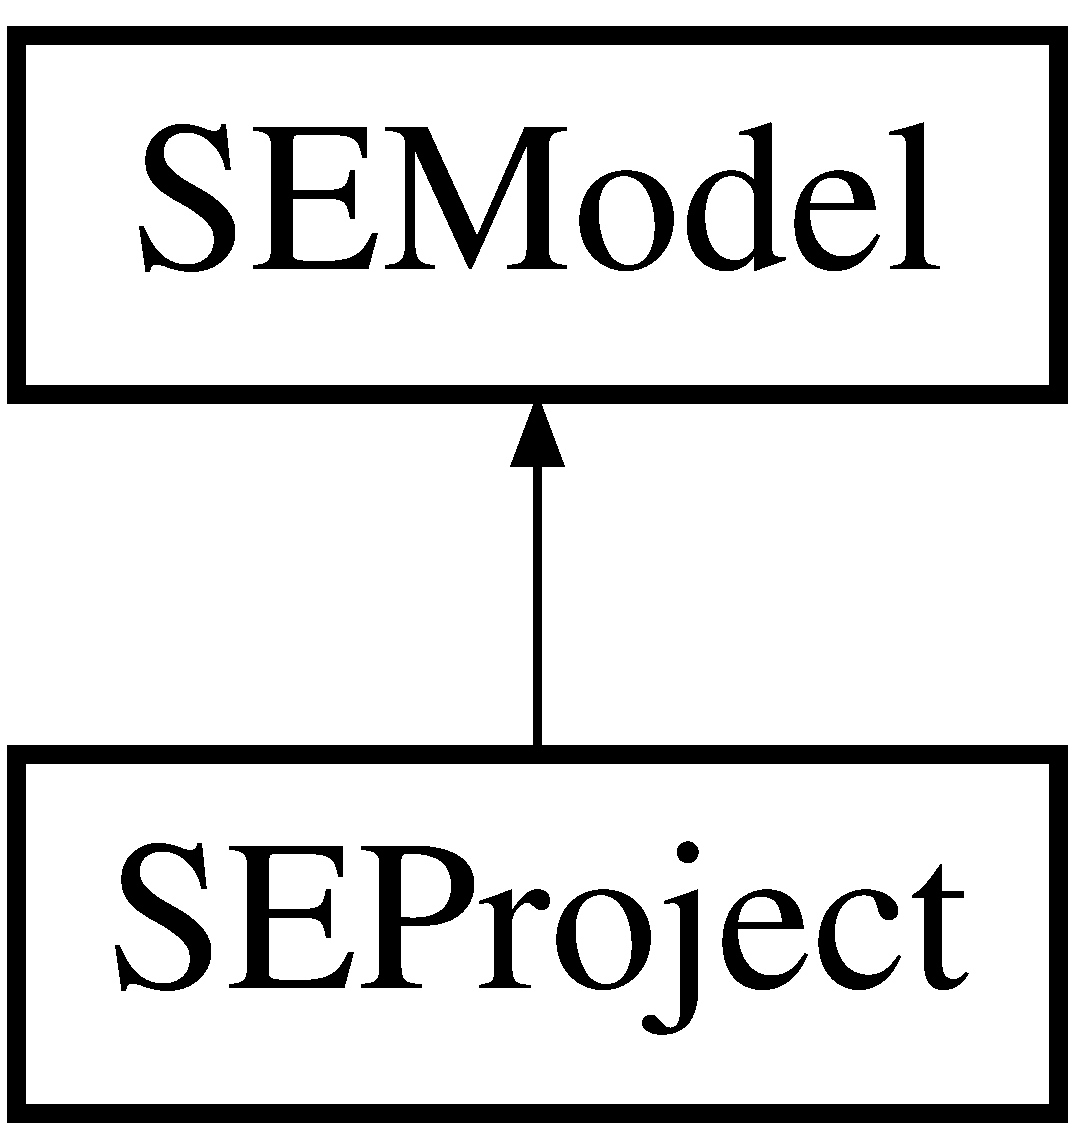
\includegraphics[height=2.000000cm]{interface_s_e_project}
\end{center}
\end{figure}
\subsection*{Instance Methods}
\begin{DoxyCompactItemize}
\item 
(\hyperlink{interface_s_e_record}{S\-E\-Record} $\ast$) -\/ \hyperlink{interface_s_e_project_adb4519610c7481bf048f235189ff737c}{split\-Record\-In\-Position\-:}
\item 
(void) -\/ \hyperlink{interface_s_e_project_a215f3b65a6214364b1c91a3e868e326f}{add\-Record\-:}
\item 
(void) -\/ \hyperlink{interface_s_e_project_a766d033976c34b25c714664a936431c0}{delete\-Record\-:}
\item 
(void) -\/ \hyperlink{interface_s_e_project_a6df677b3addadd2b57c7cb476817b3f0}{move\-Record\-:to\-Index\-:}
\item 
(void) -\/ \hyperlink{interface_s_e_project_adf1f53d931f669b12dfbabf92e3e90a4}{remove\-All\-Records}
\item 
(void) -\/ \hyperlink{interface_s_e_project_ad0dc83a89c70e8a670d2e0eb0381e632}{save\-Project}
\item 
(void) -\/ \hyperlink{interface_s_e_project_a996a39778f2d176ecf7ffda117703f6c}{save\-Project\-Asynchronously\-With\-Completion\-:}
\end{DoxyCompactItemize}
\subsection*{Properties}
\begin{DoxyCompactItemize}
\item 
N\-S\-String $\ast$ \hyperlink{interface_s_e_project_adf05552fc2cf324eb3511d3bd1b8a996}{name}
\item 
N\-S\-String $\ast$ \hyperlink{interface_s_e_project_a2d54ed4720974d226ab30b8d32ef21dd}{project\-File\-Path}
\item 
N\-S\-String $\ast$ \hyperlink{interface_s_e_project_a59726fcb927ff059c83a1ac7b252db0d}{project\-Sounds\-Path}
\item 
N\-S\-Array $\ast$ \hyperlink{interface_s_e_project_ac1f0c37f5832b2ba24ac9bf65f0fdcce}{records}
\item 
\hyperlink{interface_s_e_audio_stream_player}{S\-E\-Audio\-Stream\-Player} $\ast$ \hyperlink{interface_s_e_project_af35059bb818d498c8a96053818016a26}{audio\-Stream}
\item 
B\-O\-O\-L \hyperlink{interface_s_e_project_a4da84c0c1ef729881956646b15762cc9}{is\-Changed}
\end{DoxyCompactItemize}


\subsection{Method Documentation}
\hypertarget{interface_s_e_project_a215f3b65a6214364b1c91a3e868e326f}{\index{S\-E\-Project@{S\-E\-Project}!add\-Record\-:@{add\-Record\-:}}
\index{add\-Record\-:@{add\-Record\-:}!SEProject@{S\-E\-Project}}
\subsubsection[{add\-Record\-:}]{\setlength{\rightskip}{0pt plus 5cm}-\/ (void) add\-Record\-: 
\begin{DoxyParamCaption}
\item[{({\bf S\-E\-Record}$\ast$)}]{record}
\end{DoxyParamCaption}
}}\label{interface_s_e_project_a215f3b65a6214364b1c91a3e868e326f}
Add record to project \hypertarget{interface_s_e_project_a766d033976c34b25c714664a936431c0}{\index{S\-E\-Project@{S\-E\-Project}!delete\-Record\-:@{delete\-Record\-:}}
\index{delete\-Record\-:@{delete\-Record\-:}!SEProject@{S\-E\-Project}}
\subsubsection[{delete\-Record\-:}]{\setlength{\rightskip}{0pt plus 5cm}-\/ (void) delete\-Record\-: 
\begin{DoxyParamCaption}
\item[{({\bf S\-E\-Record}$\ast$)}]{record}
\end{DoxyParamCaption}
}}\label{interface_s_e_project_a766d033976c34b25c714664a936431c0}
Delete record from project \hypertarget{interface_s_e_project_a6df677b3addadd2b57c7cb476817b3f0}{\index{S\-E\-Project@{S\-E\-Project}!move\-Record\-:to\-Index\-:@{move\-Record\-:to\-Index\-:}}
\index{move\-Record\-:to\-Index\-:@{move\-Record\-:to\-Index\-:}!SEProject@{S\-E\-Project}}
\subsubsection[{move\-Record\-:to\-Index\-:}]{\setlength{\rightskip}{0pt plus 5cm}-\/ (void) move\-Record\-: 
\begin{DoxyParamCaption}
\item[{({\bf S\-E\-Record}$\ast$)}]{record}
\item[{toIndex:(N\-S\-Integer)}]{index}
\end{DoxyParamCaption}
}}\label{interface_s_e_project_a6df677b3addadd2b57c7cb476817b3f0}
Change records order \hypertarget{interface_s_e_project_adf1f53d931f669b12dfbabf92e3e90a4}{\index{S\-E\-Project@{S\-E\-Project}!remove\-All\-Records@{remove\-All\-Records}}
\index{remove\-All\-Records@{remove\-All\-Records}!SEProject@{S\-E\-Project}}
\subsubsection[{remove\-All\-Records}]{\setlength{\rightskip}{0pt plus 5cm}-\/ (void) remove\-All\-Records 
\begin{DoxyParamCaption}
{}
\end{DoxyParamCaption}
}}\label{interface_s_e_project_adf1f53d931f669b12dfbabf92e3e90a4}
Remove all records from project including all sound that are saved to the project sound folder \hypertarget{interface_s_e_project_ad0dc83a89c70e8a670d2e0eb0381e632}{\index{S\-E\-Project@{S\-E\-Project}!save\-Project@{save\-Project}}
\index{save\-Project@{save\-Project}!SEProject@{S\-E\-Project}}
\subsubsection[{save\-Project}]{\setlength{\rightskip}{0pt plus 5cm}-\/ (void) save\-Project 
\begin{DoxyParamCaption}
{}
\end{DoxyParamCaption}
}}\label{interface_s_e_project_ad0dc83a89c70e8a670d2e0eb0381e632}
Save project \hypertarget{interface_s_e_project_a996a39778f2d176ecf7ffda117703f6c}{\index{S\-E\-Project@{S\-E\-Project}!save\-Project\-Asynchronously\-With\-Completion\-:@{save\-Project\-Asynchronously\-With\-Completion\-:}}
\index{save\-Project\-Asynchronously\-With\-Completion\-:@{save\-Project\-Asynchronously\-With\-Completion\-:}!SEProject@{S\-E\-Project}}
\subsubsection[{save\-Project\-Asynchronously\-With\-Completion\-:}]{\setlength{\rightskip}{0pt plus 5cm}-\/ (void) save\-Project\-Asynchronously\-With\-Completion\-: 
\begin{DoxyParamCaption}
\item[{(void($^\wedge$)(N\-S\-Error$\ast$ error))}]{completion}
\end{DoxyParamCaption}
}}\label{interface_s_e_project_a996a39778f2d176ecf7ffda117703f6c}
Save project in asynchronously (in another thread) \hypertarget{interface_s_e_project_adb4519610c7481bf048f235189ff737c}{\index{S\-E\-Project@{S\-E\-Project}!split\-Record\-In\-Position\-:@{split\-Record\-In\-Position\-:}}
\index{split\-Record\-In\-Position\-:@{split\-Record\-In\-Position\-:}!SEProject@{S\-E\-Project}}
\subsubsection[{split\-Record\-In\-Position\-:}]{\setlength{\rightskip}{0pt plus 5cm}-\/ ({\bf S\-E\-Record} $\ast$) split\-Record\-In\-Position\-: 
\begin{DoxyParamCaption}
\item[{(N\-S\-Time\-Interval)}]{position}
\end{DoxyParamCaption}
}}\label{interface_s_e_project_adb4519610c7481bf048f235189ff737c}


\subsection{Property Documentation}
\hypertarget{interface_s_e_project_af35059bb818d498c8a96053818016a26}{\index{S\-E\-Project@{S\-E\-Project}!audio\-Stream@{audio\-Stream}}
\index{audio\-Stream@{audio\-Stream}!SEProject@{S\-E\-Project}}
\subsubsection[{audio\-Stream}]{\setlength{\rightskip}{0pt plus 5cm}-\/ ({\bf S\-E\-Audio\-Stream\-Player}$\ast$) audio\-Stream\hspace{0.3cm}{\ttfamily [read]}, {\ttfamily [nonatomic]}, {\ttfamily [assign]}}}\label{interface_s_e_project_af35059bb818d498c8a96053818016a26}
Project audio preview stream \hypertarget{interface_s_e_project_a4da84c0c1ef729881956646b15762cc9}{\index{S\-E\-Project@{S\-E\-Project}!is\-Changed@{is\-Changed}}
\index{is\-Changed@{is\-Changed}!SEProject@{S\-E\-Project}}
\subsubsection[{is\-Changed}]{\setlength{\rightskip}{0pt plus 5cm}-\/ (B\-O\-O\-L) is\-Changed\hspace{0.3cm}{\ttfamily [read]}, {\ttfamily [nonatomic]}, {\ttfamily [assign]}}}\label{interface_s_e_project_a4da84c0c1ef729881956646b15762cc9}
Check project if it is change (add or remove record affects that) \hypertarget{interface_s_e_project_adf05552fc2cf324eb3511d3bd1b8a996}{\index{S\-E\-Project@{S\-E\-Project}!name@{name}}
\index{name@{name}!SEProject@{S\-E\-Project}}
\subsubsection[{name}]{\setlength{\rightskip}{0pt plus 5cm}-\/ (N\-S\-String$\ast$) name\hspace{0.3cm}{\ttfamily [read]}, {\ttfamily [write]}, {\ttfamily [nonatomic]}, {\ttfamily [strong]}}}\label{interface_s_e_project_adf05552fc2cf324eb3511d3bd1b8a996}
Project name \hypertarget{interface_s_e_project_a2d54ed4720974d226ab30b8d32ef21dd}{\index{S\-E\-Project@{S\-E\-Project}!project\-File\-Path@{project\-File\-Path}}
\index{project\-File\-Path@{project\-File\-Path}!SEProject@{S\-E\-Project}}
\subsubsection[{project\-File\-Path}]{\setlength{\rightskip}{0pt plus 5cm}-\/ (N\-S\-String$\ast$) project\-File\-Path\hspace{0.3cm}{\ttfamily [read]}, {\ttfamily [write]}, {\ttfamily [nonatomic]}, {\ttfamily [strong]}}}\label{interface_s_e_project_a2d54ed4720974d226ab30b8d32ef21dd}
Project file path \hypertarget{interface_s_e_project_a59726fcb927ff059c83a1ac7b252db0d}{\index{S\-E\-Project@{S\-E\-Project}!project\-Sounds\-Path@{project\-Sounds\-Path}}
\index{project\-Sounds\-Path@{project\-Sounds\-Path}!SEProject@{S\-E\-Project}}
\subsubsection[{project\-Sounds\-Path}]{\setlength{\rightskip}{0pt plus 5cm}-\/ (N\-S\-String$\ast$) project\-Sounds\-Path\hspace{0.3cm}{\ttfamily [read]}, {\ttfamily [nonatomic]}, {\ttfamily [assign]}}}\label{interface_s_e_project_a59726fcb927ff059c83a1ac7b252db0d}
Project sounds path \hypertarget{interface_s_e_project_ac1f0c37f5832b2ba24ac9bf65f0fdcce}{\index{S\-E\-Project@{S\-E\-Project}!records@{records}}
\index{records@{records}!SEProject@{S\-E\-Project}}
\subsubsection[{records}]{\setlength{\rightskip}{0pt plus 5cm}-\/ (N\-S\-Array$\ast$) records\hspace{0.3cm}{\ttfamily [read]}, {\ttfamily [nonatomic]}, {\ttfamily [assign]}}}\label{interface_s_e_project_ac1f0c37f5832b2ba24ac9bf65f0fdcce}
List of records related to this project 

The documentation for this class was generated from the following files\-:\begin{DoxyCompactItemize}
\item 
/\-Users/igor/\-Develop/\-Develop\-Git/\-Davacon/i\-Phone/\-Sound\-Recorder/\-Classes/\-Core/\-Sound\-Editor/\hyperlink{_s_e_project_8h}{S\-E\-Project.\-h}\item 
/\-Users/igor/\-Develop/\-Develop\-Git/\-Davacon/i\-Phone/\-Sound\-Recorder/\-Classes/\-Core/\-Sound\-Editor/\hyperlink{_s_e_project_8m}{S\-E\-Project.\-m}\end{DoxyCompactItemize}

\hypertarget{category_s_e_project_07_08}{\section{S\-E\-Project() Category Reference}
\label{category_s_e_project_07_08}\index{S\-E\-Project()@{S\-E\-Project()}}
}
\subsection*{Instance Methods}
\begin{DoxyCompactItemize}
\item 
(void) -\/ \hyperlink{category_s_e_project_07_08_a2733629176d07d6e49be855ca64bc8e0}{pm\-\_\-load\-Project}
\end{DoxyCompactItemize}
\subsection*{Properties}
\begin{DoxyCompactItemize}
\item 
N\-S\-String $\ast$ \hyperlink{category_s_e_project_07_08_a1ce0384975a5debe55f63d9d89116469}{pv\-\_\-project\-Path}
\item 
S\-E\-Project\-Audio\-Stream $\ast$ \hyperlink{category_s_e_project_07_08_ac797d5923f8b64961cdaea1f08f8e35e}{pv\-\_\-stream}
\item 
N\-S\-Mutable\-Array $\ast$ \hyperlink{category_s_e_project_07_08_ae2c8be64c26691c643438545604ef2e2}{pv\-\_\-records}
\item 
B\-O\-O\-L \hyperlink{category_s_e_project_07_08_ac3ea8d84f56007c0b810c3d9bdf14192}{pv\-\_\-is\-Changed}
\end{DoxyCompactItemize}


\subsection{Method Documentation}
\hypertarget{category_s_e_project_07_08_a2733629176d07d6e49be855ca64bc8e0}{\index{S\-E\-Project()@{S\-E\-Project()}!pm\-\_\-load\-Project@{pm\-\_\-load\-Project}}
\index{pm\-\_\-load\-Project@{pm\-\_\-load\-Project}!SEProject()@{S\-E\-Project()}}
\subsubsection[{pm\-\_\-load\-Project}]{\setlength{\rightskip}{0pt plus 5cm}-\/ (void) pm\-\_\-load\-Project 
\begin{DoxyParamCaption}
{}
\end{DoxyParamCaption}
}}\label{category_s_e_project_07_08_a2733629176d07d6e49be855ca64bc8e0}


\subsection{Property Documentation}
\hypertarget{category_s_e_project_07_08_ac3ea8d84f56007c0b810c3d9bdf14192}{\index{S\-E\-Project()@{S\-E\-Project()}!pv\-\_\-is\-Changed@{pv\-\_\-is\-Changed}}
\index{pv\-\_\-is\-Changed@{pv\-\_\-is\-Changed}!SEProject()@{S\-E\-Project()}}
\subsubsection[{pv\-\_\-is\-Changed}]{\setlength{\rightskip}{0pt plus 5cm}-\/ (B\-O\-O\-L) pv\-\_\-is\-Changed\hspace{0.3cm}{\ttfamily [read]}, {\ttfamily [write]}, {\ttfamily [nonatomic]}, {\ttfamily [assign]}}}\label{category_s_e_project_07_08_ac3ea8d84f56007c0b810c3d9bdf14192}
\hypertarget{category_s_e_project_07_08_a1ce0384975a5debe55f63d9d89116469}{\index{S\-E\-Project()@{S\-E\-Project()}!pv\-\_\-project\-Path@{pv\-\_\-project\-Path}}
\index{pv\-\_\-project\-Path@{pv\-\_\-project\-Path}!SEProject()@{S\-E\-Project()}}
\subsubsection[{pv\-\_\-project\-Path}]{\setlength{\rightskip}{0pt plus 5cm}-\/ (N\-S\-String$\ast$) pv\-\_\-project\-Path\hspace{0.3cm}{\ttfamily [read]}, {\ttfamily [write]}, {\ttfamily [nonatomic]}, {\ttfamily [strong]}}}\label{category_s_e_project_07_08_a1ce0384975a5debe55f63d9d89116469}
\hypertarget{category_s_e_project_07_08_ae2c8be64c26691c643438545604ef2e2}{\index{S\-E\-Project()@{S\-E\-Project()}!pv\-\_\-records@{pv\-\_\-records}}
\index{pv\-\_\-records@{pv\-\_\-records}!SEProject()@{S\-E\-Project()}}
\subsubsection[{pv\-\_\-records}]{\setlength{\rightskip}{0pt plus 5cm}-\/ (N\-S\-Mutable\-Array$\ast$) pv\-\_\-records\hspace{0.3cm}{\ttfamily [read]}, {\ttfamily [write]}, {\ttfamily [nonatomic]}, {\ttfamily [strong]}}}\label{category_s_e_project_07_08_ae2c8be64c26691c643438545604ef2e2}
\hypertarget{category_s_e_project_07_08_ac797d5923f8b64961cdaea1f08f8e35e}{\index{S\-E\-Project()@{S\-E\-Project()}!pv\-\_\-stream@{pv\-\_\-stream}}
\index{pv\-\_\-stream@{pv\-\_\-stream}!SEProject()@{S\-E\-Project()}}
\subsubsection[{pv\-\_\-stream}]{\setlength{\rightskip}{0pt plus 5cm}-\/ (S\-E\-Project\-Audio\-Stream$\ast$) pv\-\_\-stream\hspace{0.3cm}{\ttfamily [read]}, {\ttfamily [write]}, {\ttfamily [nonatomic]}, {\ttfamily [strong]}}}\label{category_s_e_project_07_08_ac797d5923f8b64961cdaea1f08f8e35e}


The documentation for this category was generated from the following file\-:\begin{DoxyCompactItemize}
\item 
/\-Users/igor/\-Develop/\-Develop\-Git/\-Davacon/i\-Phone/\-Sound\-Recorder/\-Classes/\-Core/\-Sound\-Editor/\hyperlink{_s_e_project_8m}{S\-E\-Project.\-m}\end{DoxyCompactItemize}

\hypertarget{interface_s_e_project_engine}{\section{S\-E\-Project\-Engine Class Reference}
\label{interface_s_e_project_engine}\index{S\-E\-Project\-Engine@{S\-E\-Project\-Engine}}
}


{\ttfamily \#import $<$S\-E\-Project\-Engine.\-h$>$}

Inheritance diagram for S\-E\-Project\-Engine\-:\begin{figure}[H]
\begin{center}
\leavevmode
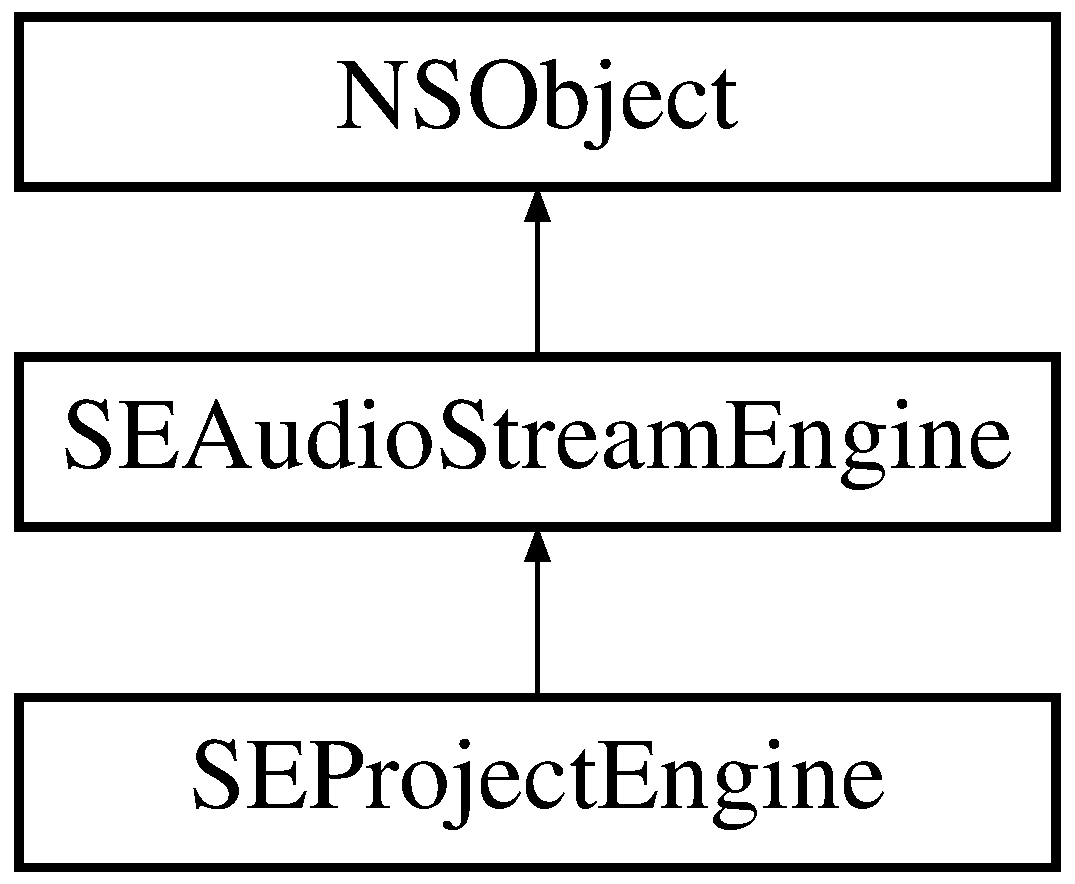
\includegraphics[height=3.000000cm]{interface_s_e_project_engine}
\end{center}
\end{figure}
\subsection*{Instance Methods}
\begin{DoxyCompactItemize}
\item 
(instancetype) -\/ \hyperlink{interface_s_e_project_engine_a7efbca25d6d786ef7d7ef089001d1c07}{init\-With\-Project\-:}
\end{DoxyCompactItemize}
\subsection*{Properties}
\begin{DoxyCompactItemize}
\item 
\hyperlink{interface_s_e_project}{S\-E\-Project} $\ast$ \hyperlink{interface_s_e_project_engine_abd99ade297e556e2e2835721016e3980}{project}
\item 
N\-S\-Time\-Interval \hyperlink{interface_s_e_project_engine_ae554c2354d873ce6d7194a8278e0acbc}{recording\-Duration}
\end{DoxyCompactItemize}


\subsection{Method Documentation}
\hypertarget{interface_s_e_project_engine_a7efbca25d6d786ef7d7ef089001d1c07}{\index{S\-E\-Project\-Engine@{S\-E\-Project\-Engine}!init\-With\-Project\-:@{init\-With\-Project\-:}}
\index{init\-With\-Project\-:@{init\-With\-Project\-:}!SEProjectEngine@{S\-E\-Project\-Engine}}
\subsubsection[{init\-With\-Project\-:}]{\setlength{\rightskip}{0pt plus 5cm}-\/ (instancetype) init\-With\-Project\-: 
\begin{DoxyParamCaption}
\item[{({\bf S\-E\-Project}$\ast$)}]{project}
\end{DoxyParamCaption}
}}\label{interface_s_e_project_engine_a7efbca25d6d786ef7d7ef089001d1c07}
Initialization with Project 

\subsection{Property Documentation}
\hypertarget{interface_s_e_project_engine_abd99ade297e556e2e2835721016e3980}{\index{S\-E\-Project\-Engine@{S\-E\-Project\-Engine}!project@{project}}
\index{project@{project}!SEProjectEngine@{S\-E\-Project\-Engine}}
\subsubsection[{project}]{\setlength{\rightskip}{0pt plus 5cm}-\/ ({\bf S\-E\-Project} $\ast$) project\hspace{0.3cm}{\ttfamily [read]}, {\ttfamily [nonatomic]}, {\ttfamily [assign]}}}\label{interface_s_e_project_engine_abd99ade297e556e2e2835721016e3980}
Pointer to audio project \hypertarget{interface_s_e_project_engine_ae554c2354d873ce6d7194a8278e0acbc}{\index{S\-E\-Project\-Engine@{S\-E\-Project\-Engine}!recording\-Duration@{recording\-Duration}}
\index{recording\-Duration@{recording\-Duration}!SEProjectEngine@{S\-E\-Project\-Engine}}
\subsubsection[{recording\-Duration}]{\setlength{\rightskip}{0pt plus 5cm}-\/ (N\-S\-Time\-Interval) recording\-Duration\hspace{0.3cm}{\ttfamily [read]}, {\ttfamily [nonatomic]}, {\ttfamily [assign]}}}\label{interface_s_e_project_engine_ae554c2354d873ce6d7194a8278e0acbc}
Recording duration 

The documentation for this class was generated from the following files\-:\begin{DoxyCompactItemize}
\item 
/\-Users/igor/\-Develop/\-Develop\-Git/\-Davacon/i\-Phone/\-Sound\-Recorder/\-Classes/\-Core/\-Sound\-Editor/\hyperlink{_s_e_project_engine_8h}{S\-E\-Project\-Engine.\-h}\item 
/\-Users/igor/\-Develop/\-Develop\-Git/\-Davacon/i\-Phone/\-Sound\-Recorder/\-Classes/\-Core/\-Sound\-Editor/\hyperlink{_s_e_project_engine_8m}{S\-E\-Project\-Engine.\-m}\end{DoxyCompactItemize}

\hypertarget{category_s_e_project_engine_07_08}{\section{S\-E\-Project\-Engine() Category Reference}
\label{category_s_e_project_engine_07_08}\index{S\-E\-Project\-Engine()@{S\-E\-Project\-Engine()}}
}
Inheritance diagram for S\-E\-Project\-Engine()\-:\begin{figure}[H]
\begin{center}
\leavevmode
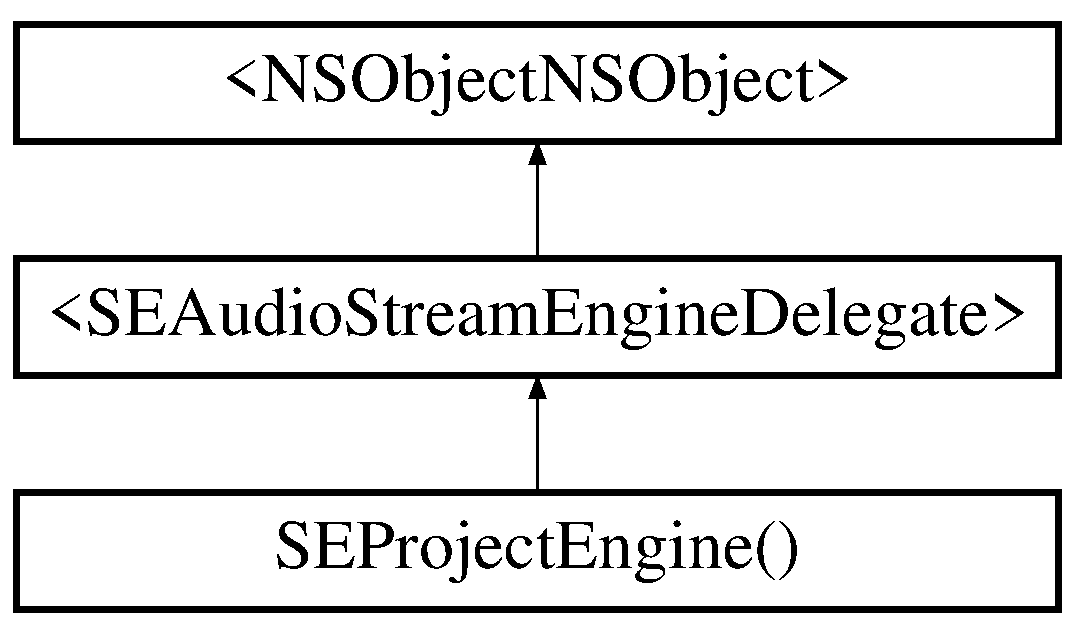
\includegraphics[height=3.000000cm]{category_s_e_project_engine_07_08}
\end{center}
\end{figure}
\subsection*{Properties}
\begin{DoxyCompactItemize}
\item 
\hyperlink{interface_s_e_project}{S\-E\-Project} $\ast$ \hyperlink{category_s_e_project_engine_07_08_a410c495fb2444cb8f4bb502819f2f709}{pv\-\_\-project}
\item 
\hyperlink{interface_s_e_audio_stream_engine}{S\-E\-Audio\-Stream\-Engine} $\ast$ \hyperlink{category_s_e_project_engine_07_08_af934c18203a994d10023f4ba3d694d5c}{pv\-\_\-recorder}
\item 
N\-S\-Time\-Interval \hyperlink{category_s_e_project_engine_07_08_ac43ef0758ea8bd82543c0af72588361f}{pv\-\_\-tmp\-Time}
\end{DoxyCompactItemize}
\subsection*{Additional Inherited Members}


\subsection{Property Documentation}
\hypertarget{category_s_e_project_engine_07_08_a410c495fb2444cb8f4bb502819f2f709}{\index{S\-E\-Project\-Engine()@{S\-E\-Project\-Engine()}!pv\-\_\-project@{pv\-\_\-project}}
\index{pv\-\_\-project@{pv\-\_\-project}!SEProjectEngine()@{S\-E\-Project\-Engine()}}
\subsubsection[{pv\-\_\-project}]{\setlength{\rightskip}{0pt plus 5cm}-\/ ({\bf S\-E\-Project}$\ast$) pv\-\_\-project\hspace{0.3cm}{\ttfamily [read]}, {\ttfamily [write]}, {\ttfamily [nonatomic]}, {\ttfamily [strong]}}}\label{category_s_e_project_engine_07_08_a410c495fb2444cb8f4bb502819f2f709}
\hypertarget{category_s_e_project_engine_07_08_af934c18203a994d10023f4ba3d694d5c}{\index{S\-E\-Project\-Engine()@{S\-E\-Project\-Engine()}!pv\-\_\-recorder@{pv\-\_\-recorder}}
\index{pv\-\_\-recorder@{pv\-\_\-recorder}!SEProjectEngine()@{S\-E\-Project\-Engine()}}
\subsubsection[{pv\-\_\-recorder}]{\setlength{\rightskip}{0pt plus 5cm}-\/ ({\bf S\-E\-Audio\-Stream\-Engine}$\ast$) pv\-\_\-recorder\hspace{0.3cm}{\ttfamily [read]}, {\ttfamily [write]}, {\ttfamily [nonatomic]}, {\ttfamily [strong]}}}\label{category_s_e_project_engine_07_08_af934c18203a994d10023f4ba3d694d5c}
\hypertarget{category_s_e_project_engine_07_08_ac43ef0758ea8bd82543c0af72588361f}{\index{S\-E\-Project\-Engine()@{S\-E\-Project\-Engine()}!pv\-\_\-tmp\-Time@{pv\-\_\-tmp\-Time}}
\index{pv\-\_\-tmp\-Time@{pv\-\_\-tmp\-Time}!SEProjectEngine()@{S\-E\-Project\-Engine()}}
\subsubsection[{pv\-\_\-tmp\-Time}]{\setlength{\rightskip}{0pt plus 5cm}-\/ (N\-S\-Time\-Interval) pv\-\_\-tmp\-Time\hspace{0.3cm}{\ttfamily [read]}, {\ttfamily [write]}, {\ttfamily [nonatomic]}, {\ttfamily [assign]}}}\label{category_s_e_project_engine_07_08_ac43ef0758ea8bd82543c0af72588361f}


The documentation for this category was generated from the following file\-:\begin{DoxyCompactItemize}
\item 
/\-Users/igor/\-Develop/\-Develop\-Git/\-Davacon/i\-Phone/\-Sound\-Recorder/\-Classes/\-Core/\-Sound\-Editor/\hyperlink{_s_e_project_engine_8m}{S\-E\-Project\-Engine.\-m}\end{DoxyCompactItemize}

\hypertarget{interface_s_e_speex_a_c_m_audio_stream}{\section{S\-E\-Speex\-A\-C\-M\-Audio\-Stream Class Reference}
\label{interface_s_e_speex_a_c_m_audio_stream}\index{S\-E\-Speex\-A\-C\-M\-Audio\-Stream@{S\-E\-Speex\-A\-C\-M\-Audio\-Stream}}
}


{\ttfamily \#import $<$S\-E\-Speex\-A\-C\-M\-Audio\-Stream.\-h$>$}

Inheritance diagram for S\-E\-Speex\-A\-C\-M\-Audio\-Stream\-:\begin{figure}[H]
\begin{center}
\leavevmode
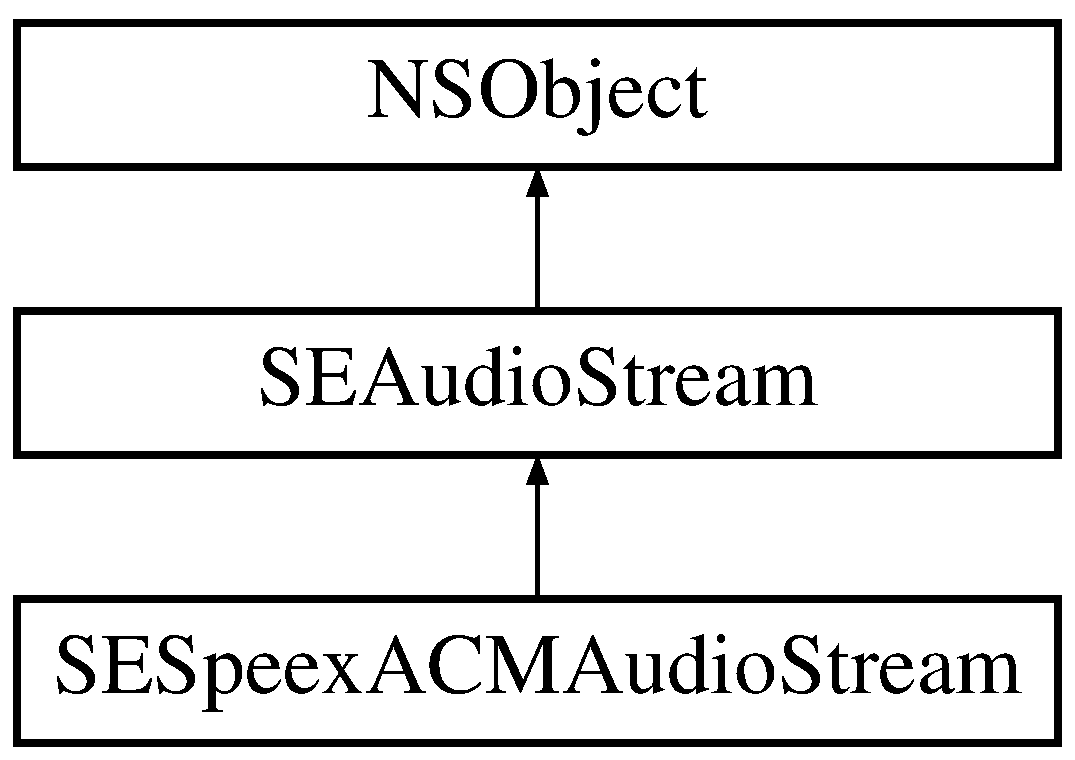
\includegraphics[height=3.000000cm]{interface_s_e_speex_a_c_m_audio_stream}
\end{center}
\end{figure}
\subsection*{Additional Inherited Members}


The documentation for this class was generated from the following file\-:\begin{DoxyCompactItemize}
\item 
/\-Users/igor/\-Develop/\-Develop\-Git/\-Davacon/i\-Phone/\-Sound\-Recorder/\-Classes/\-Core/\-Sound\-Editor/\hyperlink{_s_e_speex_a_c_m_audio_stream_8h}{S\-E\-Speex\-A\-C\-M\-Audio\-Stream.\-h}\end{DoxyCompactItemize}

\hypertarget{category_s_e_speex_a_c_m_audio_stream_07_08}{\section{S\-E\-Speex\-A\-C\-M\-Audio\-Stream() Category Reference}
\label{category_s_e_speex_a_c_m_audio_stream_07_08}\index{S\-E\-Speex\-A\-C\-M\-Audio\-Stream()@{S\-E\-Speex\-A\-C\-M\-Audio\-Stream()}}
}
\subsection*{Instance Methods}
\begin{DoxyCompactItemize}
\item 
(void) -\/ \hyperlink{category_s_e_speex_a_c_m_audio_stream_07_08_aa65035991aabcebcb8319072198e31ba}{pm\-\_\-check\-And\-Flush}
\end{DoxyCompactItemize}
\subsection*{Properties}
\begin{DoxyCompactItemize}
\item 
S\-E\-Speex\-A\-C\-M\-Wrapper $\ast$ \hyperlink{category_s_e_speex_a_c_m_audio_stream_07_08_a39c90785af2560b03827ae6e280e3338}{pv\-\_\-wrapper}
\item 
N\-S\-Mutable\-Data $\ast$ \hyperlink{category_s_e_speex_a_c_m_audio_stream_07_08_a54d58432a556297c3772d4fff8158abb}{pv\-\_\-data}
\end{DoxyCompactItemize}


\subsection{Method Documentation}
\hypertarget{category_s_e_speex_a_c_m_audio_stream_07_08_aa65035991aabcebcb8319072198e31ba}{\index{S\-E\-Speex\-A\-C\-M\-Audio\-Stream()@{S\-E\-Speex\-A\-C\-M\-Audio\-Stream()}!pm\-\_\-check\-And\-Flush@{pm\-\_\-check\-And\-Flush}}
\index{pm\-\_\-check\-And\-Flush@{pm\-\_\-check\-And\-Flush}!SESpeexACMAudioStream()@{S\-E\-Speex\-A\-C\-M\-Audio\-Stream()}}
\subsubsection[{pm\-\_\-check\-And\-Flush}]{\setlength{\rightskip}{0pt plus 5cm}-\/ (void) pm\-\_\-check\-And\-Flush 
\begin{DoxyParamCaption}
{}
\end{DoxyParamCaption}
}}\label{category_s_e_speex_a_c_m_audio_stream_07_08_aa65035991aabcebcb8319072198e31ba}


\subsection{Property Documentation}
\hypertarget{category_s_e_speex_a_c_m_audio_stream_07_08_a54d58432a556297c3772d4fff8158abb}{\index{S\-E\-Speex\-A\-C\-M\-Audio\-Stream()@{S\-E\-Speex\-A\-C\-M\-Audio\-Stream()}!pv\-\_\-data@{pv\-\_\-data}}
\index{pv\-\_\-data@{pv\-\_\-data}!SESpeexACMAudioStream()@{S\-E\-Speex\-A\-C\-M\-Audio\-Stream()}}
\subsubsection[{pv\-\_\-data}]{\setlength{\rightskip}{0pt plus 5cm}-\/ (N\-S\-Mutable\-Data$\ast$) pv\-\_\-data\hspace{0.3cm}{\ttfamily [read]}, {\ttfamily [write]}, {\ttfamily [nonatomic]}, {\ttfamily [strong]}}}\label{category_s_e_speex_a_c_m_audio_stream_07_08_a54d58432a556297c3772d4fff8158abb}
\hypertarget{category_s_e_speex_a_c_m_audio_stream_07_08_a39c90785af2560b03827ae6e280e3338}{\index{S\-E\-Speex\-A\-C\-M\-Audio\-Stream()@{S\-E\-Speex\-A\-C\-M\-Audio\-Stream()}!pv\-\_\-wrapper@{pv\-\_\-wrapper}}
\index{pv\-\_\-wrapper@{pv\-\_\-wrapper}!SESpeexACMAudioStream()@{S\-E\-Speex\-A\-C\-M\-Audio\-Stream()}}
\subsubsection[{pv\-\_\-wrapper}]{\setlength{\rightskip}{0pt plus 5cm}-\/ (S\-E\-Speex\-A\-C\-M\-Wrapper$\ast$) pv\-\_\-wrapper\hspace{0.3cm}{\ttfamily [read]}, {\ttfamily [write]}, {\ttfamily [nonatomic]}, {\ttfamily [strong]}}}\label{category_s_e_speex_a_c_m_audio_stream_07_08_a39c90785af2560b03827ae6e280e3338}


The documentation for this category was generated from the following file\-:\begin{DoxyCompactItemize}
\item 
/\-Users/igor/\-Develop/\-Develop\-Git/\-Davacon/i\-Phone/\-Sound\-Recorder/\-Classes/\-Core/\-Sound\-Editor/\hyperlink{_s_e_speex_a_c_m_audio_stream_8m}{S\-E\-Speex\-A\-C\-M\-Audio\-Stream.\-m}\end{DoxyCompactItemize}

\chapter{File Documentation}
\hypertarget{_s_e_audio_stream_8h}{\section{Sound\-Recorder/\-Classes/\-Core/\-Sound\-Editor/\-S\-E\-Audio\-Stream.h File Reference}
\label{_s_e_audio_stream_8h}\index{Sound\-Recorder/\-Classes/\-Core/\-Sound\-Editor/\-S\-E\-Audio\-Stream.\-h@{Sound\-Recorder/\-Classes/\-Core/\-Sound\-Editor/\-S\-E\-Audio\-Stream.\-h}}
}
{\ttfamily \#import $<$Audio\-Toolbox/\-Audio\-Toolbox.\-h$>$}\\*
\subsection*{Classes}
\begin{DoxyCompactItemize}
\item 
class \hyperlink{interface_s_e_audio_stream}{S\-E\-Audio\-Stream}
\item 
category \hyperlink{category_s_e_audio_stream_07_write_08}{S\-E\-Audio\-Stream(\-Write)}
\item 
category \hyperlink{category_s_e_audio_stream_07_read_08}{S\-E\-Audio\-Stream(\-Read)}
\end{DoxyCompactItemize}

\hypertarget{_s_e_audio_stream_8m}{\section{Sound\-Recorder/\-Classes/\-Core/\-Sound\-Editor/\-S\-E\-Audio\-Stream.m File Reference}
\label{_s_e_audio_stream_8m}\index{Sound\-Recorder/\-Classes/\-Core/\-Sound\-Editor/\-S\-E\-Audio\-Stream.\-m@{Sound\-Recorder/\-Classes/\-Core/\-Sound\-Editor/\-S\-E\-Audio\-Stream.\-m}}
}
{\ttfamily \#import \char`\"{}S\-E\-Audio\-Stream.\-h\char`\"{}}\\*

\hypertarget{_s_e_audio_stream_engine_8h}{\section{/\-Users/igor/\-Develop/\-Develop\-Git/\-Davacon/i\-Phone/\-Sound\-Recorder/\-Classes/\-Core/\-Sound\-Editor/\-S\-E\-Audio\-Stream\-Engine.h File Reference}
\label{_s_e_audio_stream_engine_8h}\index{/\-Users/igor/\-Develop/\-Develop\-Git/\-Davacon/i\-Phone/\-Sound\-Recorder/\-Classes/\-Core/\-Sound\-Editor/\-S\-E\-Audio\-Stream\-Engine.\-h@{/\-Users/igor/\-Develop/\-Develop\-Git/\-Davacon/i\-Phone/\-Sound\-Recorder/\-Classes/\-Core/\-Sound\-Editor/\-S\-E\-Audio\-Stream\-Engine.\-h}}
}
\subsection*{Classes}
\begin{DoxyCompactItemize}
\item 
class \hyperlink{interface_s_e_audio_stream_engine}{S\-E\-Audio\-Stream\-Engine}
\item 
protocol \hyperlink{protocol_s_e_audio_stream_engine_delegate-p}{$<$\-S\-E\-Audio\-Stream\-Engine\-Delegate$>$}
\end{DoxyCompactItemize}
\subsection*{Enumerations}
\begin{DoxyCompactItemize}
\item 
enum \hyperlink{_s_e_audio_stream_engine_8h_a6eabe41a5616eddfad154f7259ccdc27}{T\-S\-E\-Audio\-Stream\-Engine\-State} \{ \\*
\hyperlink{_s_e_audio_stream_engine_8h_a6eabe41a5616eddfad154f7259ccdc27ad62c3b56e8448412a0f2802e6f4f8160}{k\-S\-E\-Audio\-Stream\-Engine\-State\-Not\-Ready}, 
\hyperlink{_s_e_audio_stream_engine_8h_a6eabe41a5616eddfad154f7259ccdc27a61f52879bb9c0fc828cd0f2f4113c348}{k\-S\-E\-Audio\-Stream\-Engine\-State\-Ready}, 
\hyperlink{_s_e_audio_stream_engine_8h_a6eabe41a5616eddfad154f7259ccdc27a6fcacb108aa21c37435ae618a60571e5}{k\-S\-E\-Audio\-Stream\-Engine\-State\-Playing}, 
\hyperlink{_s_e_audio_stream_engine_8h_a6eabe41a5616eddfad154f7259ccdc27a8047a1c49de4e4518bb5507941ed2f55}{k\-S\-E\-Audio\-Stream\-Engine\-State\-Paused}, 
\\*
\hyperlink{_s_e_audio_stream_engine_8h_a6eabe41a5616eddfad154f7259ccdc27af0443ad2b2552b1c782ef9c5d4d08768}{k\-S\-E\-Audio\-Stream\-Engine\-State\-Recording}
 \}
\end{DoxyCompactItemize}


\subsection{Enumeration Type Documentation}
\hypertarget{_s_e_audio_stream_engine_8h_a6eabe41a5616eddfad154f7259ccdc27}{\index{S\-E\-Audio\-Stream\-Engine.\-h@{S\-E\-Audio\-Stream\-Engine.\-h}!T\-S\-E\-Audio\-Stream\-Engine\-State@{T\-S\-E\-Audio\-Stream\-Engine\-State}}
\index{T\-S\-E\-Audio\-Stream\-Engine\-State@{T\-S\-E\-Audio\-Stream\-Engine\-State}!SEAudioStreamEngine.h@{S\-E\-Audio\-Stream\-Engine.\-h}}
\subsubsection[{T\-S\-E\-Audio\-Stream\-Engine\-State}]{\setlength{\rightskip}{0pt plus 5cm}enum {\bf T\-S\-E\-Audio\-Stream\-Engine\-State}}}\label{_s_e_audio_stream_engine_8h_a6eabe41a5616eddfad154f7259ccdc27}
\begin{Desc}
\item[Enumerator]\par
\begin{description}
\index{k\-S\-E\-Audio\-Stream\-Engine\-State\-Not\-Ready@{k\-S\-E\-Audio\-Stream\-Engine\-State\-Not\-Ready}!S\-E\-Audio\-Stream\-Engine.\-h@{S\-E\-Audio\-Stream\-Engine.\-h}}\index{S\-E\-Audio\-Stream\-Engine.\-h@{S\-E\-Audio\-Stream\-Engine.\-h}!k\-S\-E\-Audio\-Stream\-Engine\-State\-Not\-Ready@{k\-S\-E\-Audio\-Stream\-Engine\-State\-Not\-Ready}}\item[{\em 
\hypertarget{_s_e_audio_stream_engine_8h_a6eabe41a5616eddfad154f7259ccdc27ad62c3b56e8448412a0f2802e6f4f8160}{k\-S\-E\-Audio\-Stream\-Engine\-State\-Not\-Ready}\label{_s_e_audio_stream_engine_8h_a6eabe41a5616eddfad154f7259ccdc27ad62c3b56e8448412a0f2802e6f4f8160}
}]\index{k\-S\-E\-Audio\-Stream\-Engine\-State\-Ready@{k\-S\-E\-Audio\-Stream\-Engine\-State\-Ready}!S\-E\-Audio\-Stream\-Engine.\-h@{S\-E\-Audio\-Stream\-Engine.\-h}}\index{S\-E\-Audio\-Stream\-Engine.\-h@{S\-E\-Audio\-Stream\-Engine.\-h}!k\-S\-E\-Audio\-Stream\-Engine\-State\-Ready@{k\-S\-E\-Audio\-Stream\-Engine\-State\-Ready}}\item[{\em 
\hypertarget{_s_e_audio_stream_engine_8h_a6eabe41a5616eddfad154f7259ccdc27a61f52879bb9c0fc828cd0f2f4113c348}{k\-S\-E\-Audio\-Stream\-Engine\-State\-Ready}\label{_s_e_audio_stream_engine_8h_a6eabe41a5616eddfad154f7259ccdc27a61f52879bb9c0fc828cd0f2f4113c348}
}]\index{k\-S\-E\-Audio\-Stream\-Engine\-State\-Playing@{k\-S\-E\-Audio\-Stream\-Engine\-State\-Playing}!S\-E\-Audio\-Stream\-Engine.\-h@{S\-E\-Audio\-Stream\-Engine.\-h}}\index{S\-E\-Audio\-Stream\-Engine.\-h@{S\-E\-Audio\-Stream\-Engine.\-h}!k\-S\-E\-Audio\-Stream\-Engine\-State\-Playing@{k\-S\-E\-Audio\-Stream\-Engine\-State\-Playing}}\item[{\em 
\hypertarget{_s_e_audio_stream_engine_8h_a6eabe41a5616eddfad154f7259ccdc27a6fcacb108aa21c37435ae618a60571e5}{k\-S\-E\-Audio\-Stream\-Engine\-State\-Playing}\label{_s_e_audio_stream_engine_8h_a6eabe41a5616eddfad154f7259ccdc27a6fcacb108aa21c37435ae618a60571e5}
}]\index{k\-S\-E\-Audio\-Stream\-Engine\-State\-Paused@{k\-S\-E\-Audio\-Stream\-Engine\-State\-Paused}!S\-E\-Audio\-Stream\-Engine.\-h@{S\-E\-Audio\-Stream\-Engine.\-h}}\index{S\-E\-Audio\-Stream\-Engine.\-h@{S\-E\-Audio\-Stream\-Engine.\-h}!k\-S\-E\-Audio\-Stream\-Engine\-State\-Paused@{k\-S\-E\-Audio\-Stream\-Engine\-State\-Paused}}\item[{\em 
\hypertarget{_s_e_audio_stream_engine_8h_a6eabe41a5616eddfad154f7259ccdc27a8047a1c49de4e4518bb5507941ed2f55}{k\-S\-E\-Audio\-Stream\-Engine\-State\-Paused}\label{_s_e_audio_stream_engine_8h_a6eabe41a5616eddfad154f7259ccdc27a8047a1c49de4e4518bb5507941ed2f55}
}]\index{k\-S\-E\-Audio\-Stream\-Engine\-State\-Recording@{k\-S\-E\-Audio\-Stream\-Engine\-State\-Recording}!S\-E\-Audio\-Stream\-Engine.\-h@{S\-E\-Audio\-Stream\-Engine.\-h}}\index{S\-E\-Audio\-Stream\-Engine.\-h@{S\-E\-Audio\-Stream\-Engine.\-h}!k\-S\-E\-Audio\-Stream\-Engine\-State\-Recording@{k\-S\-E\-Audio\-Stream\-Engine\-State\-Recording}}\item[{\em 
\hypertarget{_s_e_audio_stream_engine_8h_a6eabe41a5616eddfad154f7259ccdc27af0443ad2b2552b1c782ef9c5d4d08768}{k\-S\-E\-Audio\-Stream\-Engine\-State\-Recording}\label{_s_e_audio_stream_engine_8h_a6eabe41a5616eddfad154f7259ccdc27af0443ad2b2552b1c782ef9c5d4d08768}
}]\end{description}
\end{Desc}

\hypertarget{_s_e_audio_stream_engine_8m}{\section{/\-Users/igor/\-Develop/\-Develop\-Git/\-Davacon/i\-Phone/\-Sound\-Recorder/\-Classes/\-Core/\-Sound\-Editor/\-S\-E\-Audio\-Stream\-Engine.m File Reference}
\label{_s_e_audio_stream_engine_8m}\index{/\-Users/igor/\-Develop/\-Develop\-Git/\-Davacon/i\-Phone/\-Sound\-Recorder/\-Classes/\-Core/\-Sound\-Editor/\-S\-E\-Audio\-Stream\-Engine.\-m@{/\-Users/igor/\-Develop/\-Develop\-Git/\-Davacon/i\-Phone/\-Sound\-Recorder/\-Classes/\-Core/\-Sound\-Editor/\-S\-E\-Audio\-Stream\-Engine.\-m}}
}
{\ttfamily \#import \char`\"{}S\-E\-Audio\-Stream\-Engine.\-h\char`\"{}}\\*
{\ttfamily \#import \char`\"{}S\-E\-Audio\-Stream.\-h\char`\"{}}\\*
{\ttfamily \#import $<$A\-V\-Foundation/\-A\-V\-Foundation.\-h$>$}\\*
\subsection*{Macros}
\begin{DoxyCompactItemize}
\item 
\#define \hyperlink{_s_e_audio_stream_engine_8m_a9f85a12d6728defe2b370309f77897f4}{S\-E\-Throw\-If\-Error}(error, operation)
\end{DoxyCompactItemize}
\subsection*{Enumerations}
\begin{DoxyCompactItemize}
\item 
enum \hyperlink{_s_e_audio_stream_engine_8m_a18d86eebc9db09c928b17b2053451afa}{T\-S\-E\-Audio\-Stream\-Engine\-Error} \{ \\*
\hyperlink{_s_e_audio_stream_engine_8m_a18d86eebc9db09c928b17b2053451afaa512eb7231fca15ff98b2f8bd0a543d61}{k\-S\-E\-Audio\-Stream\-Engine\-Error\-None}, 
\hyperlink{_s_e_audio_stream_engine_8m_a18d86eebc9db09c928b17b2053451afaad35ffffae599246b8ec36cf469197033}{k\-S\-E\-Audio\-Stream\-Engine\-Error\-Cant\-Load\-Stream}, 
\hyperlink{_s_e_audio_stream_engine_8m_a18d86eebc9db09c928b17b2053451afaa72ae0337669283a89cef513f31d63c63}{k\-S\-E\-Audio\-Stream\-Engine\-Error\-Cant\-Play}, 
\hyperlink{_s_e_audio_stream_engine_8m_a18d86eebc9db09c928b17b2053451afaa434601725a79c3cd825cc7c8f1f06611}{k\-S\-E\-Audio\-Stream\-Engine\-Error\-Read\-Buffer}, 
\\*
\hyperlink{_s_e_audio_stream_engine_8m_a18d86eebc9db09c928b17b2053451afaa8cb172d08131cc0ead1fa447608a8d45}{k\-S\-E\-Audio\-Stream\-Engine\-Error\-Cant\-Pause}, 
\hyperlink{_s_e_audio_stream_engine_8m_a18d86eebc9db09c928b17b2053451afaab4e1d7b60f6cd52151b22cb52a2f0542}{k\-S\-E\-Audio\-Stream\-Engine\-Error\-Cant\-Record}, 
\hyperlink{_s_e_audio_stream_engine_8m_a18d86eebc9db09c928b17b2053451afaaf4d54fbc690bbed8655f1e43ca80a0c1}{k\-S\-E\-Audio\-Stream\-Engine\-Error\-Wrong\-Record\-Info}
 \}
\end{DoxyCompactItemize}
\subsection*{Functions}
\begin{DoxyCompactItemize}
\item 
void \hyperlink{_s_e_audio_stream_engine_8m_a76943981b7556a476fce22d07fc2eeeb}{S\-E\-Audio\-Stream\-Engine\-Output\-Buffer\-Callback} (void $\ast$in\-User\-Data, Audio\-Queue\-Ref in\-A\-Q, Audio\-Queue\-Buffer\-Ref in\-Buffer)
\item 
void \hyperlink{_s_e_audio_stream_engine_8m_ab96752aa7e79ca75e8414121714518d8}{S\-E\-Audio\-Stream\-Engine\-Input\-Buffer\-Call\-Back} (void $\ast$in\-User\-Data, Audio\-Queue\-Ref in\-A\-Q, Audio\-Queue\-Buffer\-Ref in\-Buffer, const Audio\-Time\-Stamp $\ast$in\-Start\-Time, U\-Int32 in\-Number\-Packet\-Descriptions, const Audio\-Stream\-Packet\-Description $\ast$in\-Packet\-Descs)
\end{DoxyCompactItemize}


\subsection{Macro Definition Documentation}
\hypertarget{_s_e_audio_stream_engine_8m_a9f85a12d6728defe2b370309f77897f4}{\index{S\-E\-Audio\-Stream\-Engine.\-m@{S\-E\-Audio\-Stream\-Engine.\-m}!S\-E\-Throw\-If\-Error@{S\-E\-Throw\-If\-Error}}
\index{S\-E\-Throw\-If\-Error@{S\-E\-Throw\-If\-Error}!SEAudioStreamEngine.m@{S\-E\-Audio\-Stream\-Engine.\-m}}
\subsubsection[{S\-E\-Throw\-If\-Error}]{\setlength{\rightskip}{0pt plus 5cm}\#define S\-E\-Throw\-If\-Error(
\begin{DoxyParamCaption}
\item[{}]{error, }
\item[{}]{operation}
\end{DoxyParamCaption}
)}}\label{_s_e_audio_stream_engine_8m_a9f85a12d6728defe2b370309f77897f4}
{\bfseries Value\-:}
\begin{DoxyCode}
\textcolor{keywordflow}{do} \{                                        \(\backslash\)
    if (\hyperlink{interface_s_e_audio_stream_adbfea649836caa8559708a933f907536}{error}) \{                                \(\backslash\)
        \textcolor{keyword}{@throw} @(operation);                         \(\backslash\)
    \}                                           \(\backslash\)
\} \textcolor{keywordflow}{while} (0)
\end{DoxyCode}


\subsection{Enumeration Type Documentation}
\hypertarget{_s_e_audio_stream_engine_8m_a18d86eebc9db09c928b17b2053451afa}{\index{S\-E\-Audio\-Stream\-Engine.\-m@{S\-E\-Audio\-Stream\-Engine.\-m}!T\-S\-E\-Audio\-Stream\-Engine\-Error@{T\-S\-E\-Audio\-Stream\-Engine\-Error}}
\index{T\-S\-E\-Audio\-Stream\-Engine\-Error@{T\-S\-E\-Audio\-Stream\-Engine\-Error}!SEAudioStreamEngine.m@{S\-E\-Audio\-Stream\-Engine.\-m}}
\subsubsection[{T\-S\-E\-Audio\-Stream\-Engine\-Error}]{\setlength{\rightskip}{0pt plus 5cm}enum {\bf T\-S\-E\-Audio\-Stream\-Engine\-Error}}}\label{_s_e_audio_stream_engine_8m_a18d86eebc9db09c928b17b2053451afa}
\begin{Desc}
\item[Enumerator]\par
\begin{description}
\index{k\-S\-E\-Audio\-Stream\-Engine\-Error\-None@{k\-S\-E\-Audio\-Stream\-Engine\-Error\-None}!S\-E\-Audio\-Stream\-Engine.\-m@{S\-E\-Audio\-Stream\-Engine.\-m}}\index{S\-E\-Audio\-Stream\-Engine.\-m@{S\-E\-Audio\-Stream\-Engine.\-m}!k\-S\-E\-Audio\-Stream\-Engine\-Error\-None@{k\-S\-E\-Audio\-Stream\-Engine\-Error\-None}}\item[{\em 
\hypertarget{_s_e_audio_stream_engine_8m_a18d86eebc9db09c928b17b2053451afaa512eb7231fca15ff98b2f8bd0a543d61}{k\-S\-E\-Audio\-Stream\-Engine\-Error\-None}\label{_s_e_audio_stream_engine_8m_a18d86eebc9db09c928b17b2053451afaa512eb7231fca15ff98b2f8bd0a543d61}
}]\index{k\-S\-E\-Audio\-Stream\-Engine\-Error\-Cant\-Load\-Stream@{k\-S\-E\-Audio\-Stream\-Engine\-Error\-Cant\-Load\-Stream}!S\-E\-Audio\-Stream\-Engine.\-m@{S\-E\-Audio\-Stream\-Engine.\-m}}\index{S\-E\-Audio\-Stream\-Engine.\-m@{S\-E\-Audio\-Stream\-Engine.\-m}!k\-S\-E\-Audio\-Stream\-Engine\-Error\-Cant\-Load\-Stream@{k\-S\-E\-Audio\-Stream\-Engine\-Error\-Cant\-Load\-Stream}}\item[{\em 
\hypertarget{_s_e_audio_stream_engine_8m_a18d86eebc9db09c928b17b2053451afaad35ffffae599246b8ec36cf469197033}{k\-S\-E\-Audio\-Stream\-Engine\-Error\-Cant\-Load\-Stream}\label{_s_e_audio_stream_engine_8m_a18d86eebc9db09c928b17b2053451afaad35ffffae599246b8ec36cf469197033}
}]\index{k\-S\-E\-Audio\-Stream\-Engine\-Error\-Cant\-Play@{k\-S\-E\-Audio\-Stream\-Engine\-Error\-Cant\-Play}!S\-E\-Audio\-Stream\-Engine.\-m@{S\-E\-Audio\-Stream\-Engine.\-m}}\index{S\-E\-Audio\-Stream\-Engine.\-m@{S\-E\-Audio\-Stream\-Engine.\-m}!k\-S\-E\-Audio\-Stream\-Engine\-Error\-Cant\-Play@{k\-S\-E\-Audio\-Stream\-Engine\-Error\-Cant\-Play}}\item[{\em 
\hypertarget{_s_e_audio_stream_engine_8m_a18d86eebc9db09c928b17b2053451afaa72ae0337669283a89cef513f31d63c63}{k\-S\-E\-Audio\-Stream\-Engine\-Error\-Cant\-Play}\label{_s_e_audio_stream_engine_8m_a18d86eebc9db09c928b17b2053451afaa72ae0337669283a89cef513f31d63c63}
}]\index{k\-S\-E\-Audio\-Stream\-Engine\-Error\-Read\-Buffer@{k\-S\-E\-Audio\-Stream\-Engine\-Error\-Read\-Buffer}!S\-E\-Audio\-Stream\-Engine.\-m@{S\-E\-Audio\-Stream\-Engine.\-m}}\index{S\-E\-Audio\-Stream\-Engine.\-m@{S\-E\-Audio\-Stream\-Engine.\-m}!k\-S\-E\-Audio\-Stream\-Engine\-Error\-Read\-Buffer@{k\-S\-E\-Audio\-Stream\-Engine\-Error\-Read\-Buffer}}\item[{\em 
\hypertarget{_s_e_audio_stream_engine_8m_a18d86eebc9db09c928b17b2053451afaa434601725a79c3cd825cc7c8f1f06611}{k\-S\-E\-Audio\-Stream\-Engine\-Error\-Read\-Buffer}\label{_s_e_audio_stream_engine_8m_a18d86eebc9db09c928b17b2053451afaa434601725a79c3cd825cc7c8f1f06611}
}]\index{k\-S\-E\-Audio\-Stream\-Engine\-Error\-Cant\-Pause@{k\-S\-E\-Audio\-Stream\-Engine\-Error\-Cant\-Pause}!S\-E\-Audio\-Stream\-Engine.\-m@{S\-E\-Audio\-Stream\-Engine.\-m}}\index{S\-E\-Audio\-Stream\-Engine.\-m@{S\-E\-Audio\-Stream\-Engine.\-m}!k\-S\-E\-Audio\-Stream\-Engine\-Error\-Cant\-Pause@{k\-S\-E\-Audio\-Stream\-Engine\-Error\-Cant\-Pause}}\item[{\em 
\hypertarget{_s_e_audio_stream_engine_8m_a18d86eebc9db09c928b17b2053451afaa8cb172d08131cc0ead1fa447608a8d45}{k\-S\-E\-Audio\-Stream\-Engine\-Error\-Cant\-Pause}\label{_s_e_audio_stream_engine_8m_a18d86eebc9db09c928b17b2053451afaa8cb172d08131cc0ead1fa447608a8d45}
}]\index{k\-S\-E\-Audio\-Stream\-Engine\-Error\-Cant\-Record@{k\-S\-E\-Audio\-Stream\-Engine\-Error\-Cant\-Record}!S\-E\-Audio\-Stream\-Engine.\-m@{S\-E\-Audio\-Stream\-Engine.\-m}}\index{S\-E\-Audio\-Stream\-Engine.\-m@{S\-E\-Audio\-Stream\-Engine.\-m}!k\-S\-E\-Audio\-Stream\-Engine\-Error\-Cant\-Record@{k\-S\-E\-Audio\-Stream\-Engine\-Error\-Cant\-Record}}\item[{\em 
\hypertarget{_s_e_audio_stream_engine_8m_a18d86eebc9db09c928b17b2053451afaab4e1d7b60f6cd52151b22cb52a2f0542}{k\-S\-E\-Audio\-Stream\-Engine\-Error\-Cant\-Record}\label{_s_e_audio_stream_engine_8m_a18d86eebc9db09c928b17b2053451afaab4e1d7b60f6cd52151b22cb52a2f0542}
}]\index{k\-S\-E\-Audio\-Stream\-Engine\-Error\-Wrong\-Record\-Info@{k\-S\-E\-Audio\-Stream\-Engine\-Error\-Wrong\-Record\-Info}!S\-E\-Audio\-Stream\-Engine.\-m@{S\-E\-Audio\-Stream\-Engine.\-m}}\index{S\-E\-Audio\-Stream\-Engine.\-m@{S\-E\-Audio\-Stream\-Engine.\-m}!k\-S\-E\-Audio\-Stream\-Engine\-Error\-Wrong\-Record\-Info@{k\-S\-E\-Audio\-Stream\-Engine\-Error\-Wrong\-Record\-Info}}\item[{\em 
\hypertarget{_s_e_audio_stream_engine_8m_a18d86eebc9db09c928b17b2053451afaaf4d54fbc690bbed8655f1e43ca80a0c1}{k\-S\-E\-Audio\-Stream\-Engine\-Error\-Wrong\-Record\-Info}\label{_s_e_audio_stream_engine_8m_a18d86eebc9db09c928b17b2053451afaaf4d54fbc690bbed8655f1e43ca80a0c1}
}]\end{description}
\end{Desc}


\subsection{Function Documentation}
\hypertarget{_s_e_audio_stream_engine_8m_ab96752aa7e79ca75e8414121714518d8}{\index{S\-E\-Audio\-Stream\-Engine.\-m@{S\-E\-Audio\-Stream\-Engine.\-m}!S\-E\-Audio\-Stream\-Engine\-Input\-Buffer\-Call\-Back@{S\-E\-Audio\-Stream\-Engine\-Input\-Buffer\-Call\-Back}}
\index{S\-E\-Audio\-Stream\-Engine\-Input\-Buffer\-Call\-Back@{S\-E\-Audio\-Stream\-Engine\-Input\-Buffer\-Call\-Back}!SEAudioStreamEngine.m@{S\-E\-Audio\-Stream\-Engine.\-m}}
\subsubsection[{S\-E\-Audio\-Stream\-Engine\-Input\-Buffer\-Call\-Back}]{\setlength{\rightskip}{0pt plus 5cm}void S\-E\-Audio\-Stream\-Engine\-Input\-Buffer\-Call\-Back (
\begin{DoxyParamCaption}
\item[{void $\ast$}]{in\-User\-Data, }
\item[{Audio\-Queue\-Ref}]{in\-A\-Q, }
\item[{Audio\-Queue\-Buffer\-Ref}]{in\-Buffer, }
\item[{const Audio\-Time\-Stamp $\ast$}]{in\-Start\-Time, }
\item[{U\-Int32}]{in\-Number\-Packet\-Descriptions, }
\item[{const Audio\-Stream\-Packet\-Description $\ast$}]{in\-Packet\-Descs}
\end{DoxyParamCaption}
)}}\label{_s_e_audio_stream_engine_8m_ab96752aa7e79ca75e8414121714518d8}
\hypertarget{_s_e_audio_stream_engine_8m_a76943981b7556a476fce22d07fc2eeeb}{\index{S\-E\-Audio\-Stream\-Engine.\-m@{S\-E\-Audio\-Stream\-Engine.\-m}!S\-E\-Audio\-Stream\-Engine\-Output\-Buffer\-Callback@{S\-E\-Audio\-Stream\-Engine\-Output\-Buffer\-Callback}}
\index{S\-E\-Audio\-Stream\-Engine\-Output\-Buffer\-Callback@{S\-E\-Audio\-Stream\-Engine\-Output\-Buffer\-Callback}!SEAudioStreamEngine.m@{S\-E\-Audio\-Stream\-Engine.\-m}}
\subsubsection[{S\-E\-Audio\-Stream\-Engine\-Output\-Buffer\-Callback}]{\setlength{\rightskip}{0pt plus 5cm}void S\-E\-Audio\-Stream\-Engine\-Output\-Buffer\-Callback (
\begin{DoxyParamCaption}
\item[{void $\ast$}]{in\-User\-Data, }
\item[{Audio\-Queue\-Ref}]{in\-A\-Q, }
\item[{Audio\-Queue\-Buffer\-Ref}]{in\-Buffer}
\end{DoxyParamCaption}
)}}\label{_s_e_audio_stream_engine_8m_a76943981b7556a476fce22d07fc2eeeb}

\hypertarget{_s_e_project_8h}{\section{/\-Users/igor/\-Develop/\-Develop\-Git/\-Davacon/i\-Phone/\-Sound\-Recorder/\-Classes/\-Core/\-Sound\-Editor/\-S\-E\-Project.h File Reference}
\label{_s_e_project_8h}\index{/\-Users/igor/\-Develop/\-Develop\-Git/\-Davacon/i\-Phone/\-Sound\-Recorder/\-Classes/\-Core/\-Sound\-Editor/\-S\-E\-Project.\-h@{/\-Users/igor/\-Develop/\-Develop\-Git/\-Davacon/i\-Phone/\-Sound\-Recorder/\-Classes/\-Core/\-Sound\-Editor/\-S\-E\-Project.\-h}}
}
{\ttfamily \#import \char`\"{}S\-E\-Model.\-h\char`\"{}}\\*
{\ttfamily \#import \char`\"{}S\-E\-Audio\-Stream\-Player.\-h\char`\"{}}\\*
{\ttfamily \#import \char`\"{}S\-E\-Record.\-h\char`\"{}}\\*
\subsection*{Classes}
\begin{DoxyCompactItemize}
\item 
class \hyperlink{interface_s_e_project}{S\-E\-Project}
\end{DoxyCompactItemize}

\hypertarget{_s_e_project_8m}{\section{/\-Users/igor/\-Develop/\-Develop\-Git/\-Davacon/i\-Phone/\-Sound\-Recorder/\-Classes/\-Core/\-Sound\-Editor/\-S\-E\-Project.m File Reference}
\label{_s_e_project_8m}\index{/\-Users/igor/\-Develop/\-Develop\-Git/\-Davacon/i\-Phone/\-Sound\-Recorder/\-Classes/\-Core/\-Sound\-Editor/\-S\-E\-Project.\-m@{/\-Users/igor/\-Develop/\-Develop\-Git/\-Davacon/i\-Phone/\-Sound\-Recorder/\-Classes/\-Core/\-Sound\-Editor/\-S\-E\-Project.\-m}}
}
{\ttfamily \#import \char`\"{}S\-E\-Project.\-h\char`\"{}}\\*
{\ttfamily \#import \char`\"{}S\-E\-Record.\-h\char`\"{}}\\*
{\ttfamily \#import \char`\"{}S\-E\-Project+\-Internal.\-h\char`\"{}}\\*

\hypertarget{_s_e_project_engine_8h}{\section{/\-Users/igor/\-Develop/\-Develop\-Git/\-Davacon/i\-Phone/\-Sound\-Recorder/\-Classes/\-Core/\-Sound\-Editor/\-S\-E\-Project\-Engine.h File Reference}
\label{_s_e_project_engine_8h}\index{/\-Users/igor/\-Develop/\-Develop\-Git/\-Davacon/i\-Phone/\-Sound\-Recorder/\-Classes/\-Core/\-Sound\-Editor/\-S\-E\-Project\-Engine.\-h@{/\-Users/igor/\-Develop/\-Develop\-Git/\-Davacon/i\-Phone/\-Sound\-Recorder/\-Classes/\-Core/\-Sound\-Editor/\-S\-E\-Project\-Engine.\-h}}
}
{\ttfamily \#import \char`\"{}S\-E\-Audio\-Stream\-Engine.\-h\char`\"{}}\\*
\subsection*{Classes}
\begin{DoxyCompactItemize}
\item 
class \hyperlink{interface_s_e_project_engine}{S\-E\-Project\-Engine}
\end{DoxyCompactItemize}

\hypertarget{_s_e_project_engine_8m}{\section{/\-Users/igor/\-Develop/\-Develop\-Git/\-Davacon/i\-Phone/\-Sound\-Recorder/\-Classes/\-Core/\-Sound\-Editor/\-S\-E\-Project\-Engine.m File Reference}
\label{_s_e_project_engine_8m}\index{/\-Users/igor/\-Develop/\-Develop\-Git/\-Davacon/i\-Phone/\-Sound\-Recorder/\-Classes/\-Core/\-Sound\-Editor/\-S\-E\-Project\-Engine.\-m@{/\-Users/igor/\-Develop/\-Develop\-Git/\-Davacon/i\-Phone/\-Sound\-Recorder/\-Classes/\-Core/\-Sound\-Editor/\-S\-E\-Project\-Engine.\-m}}
}
{\ttfamily \#import \char`\"{}S\-E\-Project\-Engine.\-h\char`\"{}}\\*
{\ttfamily \#import \char`\"{}S\-E\-Project.\-h\char`\"{}}\\*
{\ttfamily \#import \char`\"{}S\-E\-Project+\-Internal.\-h\char`\"{}}\\*
{\ttfamily \#import \char`\"{}S\-E\-Audio\-Stream\-Engine+\-Internal.\-h\char`\"{}}\\*

\hypertarget{_s_e_speex_a_c_m_audio_stream_8h}{\section{/\-Users/igor/\-Develop/\-Develop\-Git/\-Davacon/i\-Phone/\-Sound\-Recorder/\-Classes/\-Core/\-Sound\-Editor/\-S\-E\-Speex\-A\-C\-M\-Audio\-Stream.h File Reference}
\label{_s_e_speex_a_c_m_audio_stream_8h}\index{/\-Users/igor/\-Develop/\-Develop\-Git/\-Davacon/i\-Phone/\-Sound\-Recorder/\-Classes/\-Core/\-Sound\-Editor/\-S\-E\-Speex\-A\-C\-M\-Audio\-Stream.\-h@{/\-Users/igor/\-Develop/\-Develop\-Git/\-Davacon/i\-Phone/\-Sound\-Recorder/\-Classes/\-Core/\-Sound\-Editor/\-S\-E\-Speex\-A\-C\-M\-Audio\-Stream.\-h}}
}
{\ttfamily \#import \char`\"{}S\-E\-Audio\-Stream.\-h\char`\"{}}\\*
\subsection*{Classes}
\begin{DoxyCompactItemize}
\item 
class \hyperlink{interface_s_e_speex_a_c_m_audio_stream}{S\-E\-Speex\-A\-C\-M\-Audio\-Stream}
\end{DoxyCompactItemize}

\hypertarget{_s_e_speex_a_c_m_audio_stream_8m}{\section{/\-Users/igor/\-Develop/\-Develop\-Git/\-Davacon/i\-Phone/\-Sound\-Recorder/\-Classes/\-Core/\-Sound\-Editor/\-S\-E\-Speex\-A\-C\-M\-Audio\-Stream.m File Reference}
\label{_s_e_speex_a_c_m_audio_stream_8m}\index{/\-Users/igor/\-Develop/\-Develop\-Git/\-Davacon/i\-Phone/\-Sound\-Recorder/\-Classes/\-Core/\-Sound\-Editor/\-S\-E\-Speex\-A\-C\-M\-Audio\-Stream.\-m@{/\-Users/igor/\-Develop/\-Develop\-Git/\-Davacon/i\-Phone/\-Sound\-Recorder/\-Classes/\-Core/\-Sound\-Editor/\-S\-E\-Speex\-A\-C\-M\-Audio\-Stream.\-m}}
}
{\ttfamily \#import \char`\"{}S\-E\-Speex\-A\-C\-M\-Audio\-Stream.\-h\char`\"{}}\\*
{\ttfamily \#import \char`\"{}S\-E\-Speex\-A\-C\-M\-Wrapper.\-h\char`\"{}}\\*
{\ttfamily \#import \char`\"{}S\-E\-Audio\-Stream+\-Internal.\-h\char`\"{}}\\*

%--- End generated contents ---

% Index
\newpage
\phantomsection
\addcontentsline{toc}{chapter}{Index}
\printindex

\end{document}
